\documentclass[letterpaper,10pt]{book}
% Change to 10 pt
\usepackage{pdfpages}
\usepackage{morewrites}			% to counteract the no write space problem
\setcounter{tocdepth}{6}

\usepackage[framemethod=TikZ]{mdframed}

\usepackage{fancyhdr}

\usepackage{paralist}
\usepackage{amsmath}
\usepackage{amsfonts}
\usepackage{amssymb}
\usepackage{graphicx}

\usepackage{datetime}
%\usepackage{ulem}

%\usepackage[nottoc]{toobibind}

\usepackage[inline]{enumitem}

% Outer margin at 2.50 is exacty correct to fit the ``corruption alert'' tables
\usepackage[inner=1.0in, outer=2.50in, top=2.54cm,bottom=2.54cm, marginparwidth=2.25in]{geometry}

\usepackage{marginnote}
\usepackage{longtable}
\usepackage{booktabs}
\usepackage{xcolor}

\usepackage{soul}

%%%%%%%%%%%%
\definecolor{ForestGreen}{rgb}{0.00,0.29,0.098}
%%%%%%%%%%%%

\usepackage{marginnote}

\usepackage{imakeidx} 
\usepackage[
	backref=true,
	style=numeric,
%	citestyle=numeric,
	backend=bibtex
	]{biblatex}
\usepackage[driverfallback=hypertex,colorlinks=True]{hyperref}
\usepackage{cleveref}

\makeindex[name=scripture,columnsep=20pt, columnseprule=True,columns=3, title=Scripture References]
\makeindex[name=speaker,columnsep=20pt, columnseprule=True,,columns=2, title=Sermon Creator]
\makeindex[name=series,columnsep=20pt, columnseprule=True,,columns=2, title=Sermon Series]
\makeindex[name=date,columnsep=20pt, columnseprule=True,columns=2, title=Sermon Date]
\makeindex[name=event,columnsep=20pt, columnseprule=True,columns=2, title=Event]
\makeindex[name=topic,columnsep=20pt, columnseprule=True,columns=2, title=Topic]
\makeindex[name=AWIP,columnsep=20pt, columnseprule=True,columns=3, title=All Words in Passage]
\makeindex[name=NWIV,columnsep=20pt, columnseprule=True,columns=3, title=Number of Words in Verse]
\makeindex[name=PNIP,columnsep=20pt, columnseprule=True,columns=3, title=Proper Names in Passage]
\makeindex[name=PEIP,columnsep=20pt, columnseprule=True,columns=2, title=Prophetic Events in Passage]
\makeindex[name=TWPAQ,columnsep=20pt, columnseprule=True,columns=1, title=13-Word Phrases and Quotes]
\makeindex[name=PFTTIS,columnsep=20pt, columnseprule=False,columns=3, title=Phrases found 13 times in scripture]
\makeindex[name=WFTTIS,columnsep=20pt, columnseprule=False,columns=3, title=Words found 13 times in scripture]
\makeindex[name=WFITV,columnsep=20pt, columnseprule=False,columns=3, title=Words found in exactly 13 verses]
\makeindex[name=EVENTS,columnsep=20pt, columnseprule=False,columns=2, title=Sermon Log by Place]
\makeindex[name=QUESTIONS,columnsep=20pt, columnseprule=False,columns=2, title=Bible Questions]
\makeindex[name=DOCTRINES,columnsep=20pt, columnseprule=False,columns=2, title=Doctrines]
\makeindex[name=SONGS,columnsep=20pt, columnseprule=False,columns=1, title=Songs]
\makeindex[name=LOCATION,columnsep=20pt, columnseprule=False,columns= 2, title=Location]
\makeindex[name=FACEBOOK,columnsep=20pt, columnseprule=False,columns=2, title=Facebook]
\makeindex[name=DEVOTIONAL,columnsep=20pt, columnseprule=False,columns=2, title=Devotional Items]
%%%%%%%%%%%%%%%%% EXTRA COLORS
\definecolor{champagne}{rgb}{0.97,0.91,0.81}
\definecolor{bone}{rgb}{0.89,0.85,0.79}
\pagestyle{fancy}
\fancyhf{}
\fancyhead[LE,RO]{\today}
\fancyhead[RE,LO]{Daily Bible Reading}
\fancyhead[CE,CO]{-page \thepage  - }

\fancyfoot[CO,CE]{\leftmark}
%\fancyfoot[LE,RO]{CSCE 692, HW1}

\title{DBR\\
Daily \\ Reads}
\author{Keith Anthony \\
\today }
%+/ffffff +   \pagenumbering{gobble}
\bibliography{Bibliographies/All20220122}

\setlength{\fboxsep}{1.0pt}

\usepackage[utf8]{inputenc}
\usepackage{tikz}

\begin{document}
%%%%%%%%%%%% Tile Page

\begin{titlepage}

\begin{flushright}
\rightskip=-2.5cm
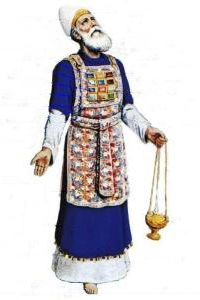
\includegraphics[width=50mm,scale=1.5]{Extras/Melchisedec.jpg}
\vspace{0.4in}  % Create a title for the document and write it in bold font
\LARGE{\textbf{\date}} % Again, do a line break
\linebreak 
% Create a subtitle \large{with Outlines, Statistics, Cross References, and Notes}
\vspace{0.5in}
\begin{flushleft}
\LARGE{Day \#80: Monday, 21  March 2022  \\}\vspace{0.25in}
\LARGE{Ruth 1-2 Psalm 80 Proverb 21}
\end{flushleft}
\vspace{0.6in}
\bigskip

\normalsize{Xenia, Oh.\\}
\normalsize{created: \today}
\vspace{1.3in}

\end{flushright}
\end{titlepage}

\newpage 
\tableofcontents\hypertarget{TOC}{}
\listoffigures
\listoftables

\hyphenation{A-bim-e-lech bre-thren E-phra-im  Gib-e-o-nites Jer-u-sa-lem through-out Phil-i-stines The-o-phil-us Am-a-le-kites ven-geance Mesh-el-e-mi-ah onan-ism Phar-a-oh thoughts grev-ous-ness Hach-a-liah adul-ter-er Shad-rach}

%%%%%%%%%%%%%%%%% EXTRA COLORS
%%%%%%%%%%%%%%%%% EXTRA COLORS
%%%%%%%%%%%%%%%%% EXTRA COLORS
\definecolor{champagne}{rgb}{0.97,0.91,0.81}
\definecolor{bone}{rgb}{0.89,0.85,0.79}

\definecolor{ForestGreen}{rgb}{0.00,0.29,0.098}
\definecolor{GIVING}{cmyk}{1,0.0,0.72,.1}

\definecolor{MLPE}{cmyk}{1,1,0,.45}
\definecolor{SOCCER}{cmyk}{.77, 0, .42, .49}
\definecolor{PAYBILL}{cmyk}{0,0.83,0.76,0.07}
\definecolor{SERMON}{cmyk}{.14,.9,0,.30} % aka seance \href{http://www.flatuicolorpicker.com/purple-cmyk-color-model/}{seance}
\definecolor{BIBLE}{cmyk}{0,.17,.74,.17}
\definecolor{WORKBLUE}{cmyk}{1, .5, 0, .6}
\definecolor{myOrange}{cmyk}{0, .4, .98, .03}
\definecolor{myTan}{cmyk}{0.0,.07,.17,.10}
\definecolor{myRed}{cmyk}{0,1,1,0}
\definecolor{myWhite}{cmyk}{0,0,0,0}
\definecolor{BLUESoD}{cmyk}{.97,.84,0,.04}
\definecolor{WHITE}{cmyk}{0,0,0,0}
\definecolor{OLDGOLD}{cmyk}{0.05,0.3,1.00,0}
\definecolor{CASTLETON}{cmyk}{1,0,0.31,0.66}
\definecolor{cadmiumgreen}{rgb}{0.0, 0.42, 0.24}
\definecolor{jungle}{rgb}{0.203,0.4882,0.1718}
\definecolor{MYGOLD}{rgb}{1,.84,0}

\definecolor{MYLIGHTGRAY}{rgb}{.85,.85,.85}

\definecolor{codegreen}{rgb}{0,0.6,0}
\definecolor{codegray}{rgb}{0.5,0.5,0.5}
\definecolor{codepurple}{rgb}{0.58,0,0.82}
\definecolor{backcolour}{rgb}{0.95,0.95,0.92}


\mdfdefinestyle{MyFrame}{%
    linecolor=blue,
    outerlinewidth=2pt,
    roundcorner=5pt,
    innertopmargin=\baselineskip,
    innerbottommargin=\baselineskip,
    innerrightmargin=10pt,
    innerleftmargin=10pt,
    backgroundcolor=gray!25!white}


\mdfdefinestyle{MyFrame2}{%
    linecolor=black,
    outerlinewidth=2pt,
    roundcorner=5pt,
    innertopmargin=\baselineskip,
    innerbottommargin=\baselineskip,
    innerrightmargin=10pt,
    innerleftmargin=10pt,
    backgroundcolor=yellow!25!white}


%%%%%
%% for PFTTIS list
%%%%%

%%% And Joseph said unto
\index[PFTTIS]{And Joseph said unto!Genesis!Gen 40:008}
\index[PFTTIS]{And Joseph said unto!Genesis!Gen 40:012}
\index[PFTTIS]{And Joseph said unto!Genesis!Gen 41:025}
\index[PFTTIS]{And Joseph said unto!Genesis!Gen 42:014}
\index[PFTTIS]{And Joseph said unto!Genesis!Gen 42:018}
\index[PFTTIS]{And Joseph said unto!Genesis!Gen 44:015}
\index[PFTTIS]{And Joseph said unto!Genesis!Gen 45:003}
\index[PFTTIS]{And Joseph said unto!Genesis!Gen 45:004}
\index[PFTTIS]{And Joseph said unto!Genesis!Gen 46:031}
\index[PFTTIS]{And Joseph said unto!Genesis!Gen 48:009}
\index[PFTTIS]{And Joseph said unto!Genesis!Gen 48:018}
\index[PFTTIS]{And Joseph said unto!Genesis!Gen 50:019}
\index[PFTTIS]{And Joseph said unto!Genesis!Gen 50:024}


%%% a shadow
\index[PFTTIS]{a shadow!1Chronicles!1Chr 029:15}
\index[PFTTIS]{a shadow!Job!Job 008:09}
\index[PFTTIS]{a shadow!Job!Job 014:02}
\index[PFTTIS]{a shadow!Job!Job 017:07}
\index[PFTTIS]{a shadow!Psalm!Psa 102:011}
\index[PFTTIS]{a shadow!Psalm!Psa 144:004}
\index[PFTTIS]{a shadow!Ecclesiastes!Eccl 006:012}
\index[PFTTIS]{a shadow!Ecclesiastes!Eccl 008:013}
\index[PFTTIS]{a shadow!Isaiah!Isa 04:006}
\index[PFTTIS]{a shadow!Isaiah!Isa 25:004}
\index[PFTTIS]{a shadow!Jonah!Jnh 04:06}
\index[PFTTIS]{a shadow!Colossians!Col 02:017}
\index[PFTTIS]{a shadow!Hebews!Heb 10:001}

%%% blessed is the man
\index[PFTTIS]{blessed is the man!Psalm!Psa 001:001}
\index[PFTTIS]{blessed is the man!Psalm!Psa 032:002}
\index[PFTTIS]{blessed is the man!Psalm!Psa 034:008}
\index[PFTTIS]{blessed is the man!Psalm!Psa 065:004}
\index[PFTTIS]{blessed is the man!Psalm!Psa 084:005}
\index[PFTTIS]{blessed is the man!Psalm!Psa 084:012}
\index[PFTTIS]{blessed is the man!Psalm!Psa 094:012}
\index[PFTTIS]{blessed is the man!Psalm!Psa 112:001}
\index[PFTTIS]{blessed is the man!Proverbs!Pro 008:034}
\index[PFTTIS]{blessed is the man!Isaiah!Isa 056:002}
\index[PFTTIS]{blessed is the man!Jeremiah!Jer 017:007}
\index[PFTTIS]{blessed is the man!Romans!Rom 004:008}
\index[PFTTIS]{blessed is the man!James!Jam 001:012}


%%% carry them
\index[PFTTIS]{carry them!Leviticus!Lev 14:045}
\index[PFTTIS]{carry them!Numbers!Num 11:012}
\index[PFTTIS]{carry them!Joshua!Jsh 04:003}
\index[PFTTIS]{carry them!1Samuel!1Sam 20:040}
\index[PFTTIS]{carry them!1Kings!1Kng 08:046}
\index[PFTTIS]{carry them!2Chronicles!2Chr 06:036}
\index[PFTTIS]{carry them!Ezra!Ezra 05:015}
\index[PFTTIS]{carry them!Isaiah!Isa 40:011}
\index[PFTTIS]{carry them!Isaiah!Isa 41:016}
\index[PFTTIS]{carry them!Isaiah!Isa 57:013}
\index[PFTTIS]{carry them!Jeremiah!Jer 20:004}
\index[PFTTIS]{carry them!Jeremiah!Jer 20:005}
\index[PFTTIS]{carry them!Jeremiah!Jer 43:012}


\index[PFTTIS]{good tidings!2Samuel!2Sam 18:027}
\index[PFTTIS]{good tidings!1Kings!1Ki 01:042}
\index[PFTTIS]{good tidings!2Kings!2Ki 07:009 (2x)}
\index[PFTTIS]{good tidings!Isaiah!Isa 40:009 (2x)}
\index[PFTTIS]{good tidings!Isaiah!Isa 41:007}
\index[PFTTIS]{good tidings!Isaiah!Isa 52:007}
\index[PFTTIS]{good tidings!Isaiah!Isa 61:001}
\index[PFTTIS]{good tidings!Nahum!Nah 01:005}
\index[PFTTIS]{good tidings!Luke!Lk 02:010}
\index[PFTTIS]{good tidings!1Thessalonians!1Thess 03:006}


%%% dead body
\index[PFTTIS]{dead body!Leviticus!Lev 21:011}
\index[PFTTIS]{dead body!Numbers!Num 06:006}
\index[PFTTIS]{dead body!Numbers!Num 09:006}
\index[PFTTIS]{dead body!Numbers!Num 09:007}
\index[PFTTIS]{dead body!Numbers!Num 09:010}
\index[PFTTIS]{dead body!Numbers!Num 09:011}
\index[PFTTIS]{dead body!Numbers!Num 09:013}
\index[PFTTIS]{dead body!Numbers!Num 09:016}
\index[PFTTIS]{dead body!2Kings!2Ki 08:005}
\index[PFTTIS]{dead body!Isaiah!Isa 26:019}
\index[PFTTIS]{dead body!Jeremiah!Jer 26:023}
\index[PFTTIS]{dead body!Jeremiah!Jer 36:030}
\index[PFTTIS]{dead body!Haggai!Hag 02:013}

%%% great sea
\index[PFTTIS]{great sea!Numbers!Num 34:006}
\index[PFTTIS]{great sea!Numbers!Num 34:007}
\index[PFTTIS]{great sea!Joshua!Jos 01:004}
\index[PFTTIS]{great sea!Joshua!Jos 09:001}
\index[PFTTIS]{great sea!Joshua!Jos 15:012}
\index[PFTTIS]{great sea!Joshua!Jos 15:047}
\index[PFTTIS]{great sea!Joshua!Jos 23:004}
\index[PFTTIS]{great sea!Ezekiel!Eze 47:010}
\index[PFTTIS]{great sea!Ezekiel!Eze 47:015}
\index[PFTTIS]{great sea!Ezekiel!Eze 47:019}
\index[PFTTIS]{great sea!Ezekiel!Eze 47:020}
\index[PFTTIS]{great sea!Ezekiel!Eze 48:028}
\index[PFTTIS]{great sea!Daniel!Dan 07:002}


%%% have forsaken me
\index[PFTTIS]{have forsaken me!Judges!Jdg 10:013}
\index[PFTTIS]{have forsaken me!1Samuel!1Sam 08:008}
\index[PFTTIS]{have forsaken me!1Kings!1Ki 11:033}
\index[PFTTIS]{have forsaken me!2Kings!2Ki 22:017}
\index[PFTTIS]{have forsaken me!2Chronicles!2Chr 12:005}
\index[PFTTIS]{have forsaken me!2Chronicles!2Chr 34:025}
\index[PFTTIS]{have forsaken me!Jeremiah!Jer 01:016}
\index[PFTTIS]{have forsaken me!Jeremiah!Jer 02:013}
\index[PFTTIS]{have forsaken me!Jeremiah!Jer 05:007}
\index[PFTTIS]{have forsaken me!Jeremiah!Jer 05:019}
\index[PFTTIS]{have forsaken me!Jeremiah!Jer 16:011 (2x)}
\index[PFTTIS]{have forsaken me!Jeremiah!Jer 19:004}

%%% no king
\index[PFTTIS]{no king!Judges!Jdg 17:06}
\index[PFTTIS]{no king!Judges!Jdg 18:01}
\index[PFTTIS]{no king!Judges!Jdg 19:01}
\index[PFTTIS]{no king!Judges!Jdg 21:25}
\index[PFTTIS]{no king!1Kings!1Ki 22:47}
\index[PFTTIS]{no king!2Kings!2Ki 23:25}
\index[PFTTIS]{no king!Nehemiah!Neh 13:26}
\index[PFTTIS]{no king!Psalms!Psa 033:016}
\index[PFTTIS]{no king!Proverbs!Pro 30:27}
\index[PFTTIS]{no king!Daniel!Dan 02:10}
\index[PFTTIS]{no king!Hosea!Hos 10:03}
\index[PFTTIS]{no king!Micah!Mic 04:09}
\index[PFTTIS]{no king!John!Jhn 19:15}


%%% rebellious house
\index[PFTTIS]{rebellious house!Exodus!Exo 02:005}
\index[PFTTIS]{rebellious house!Exodus!Exo 02:006}
\index[PFTTIS]{rebellious house!Exodus!Exo 02:008}
\index[PFTTIS]{rebellious house!Exodus!Exo 03:009}
\index[PFTTIS]{rebellious house!Exodus!Exo 03:026}
\index[PFTTIS]{rebellious house!Exodus!Exo 03:027}
\index[PFTTIS]{rebellious house!Exodus!Exo 12:002 (2x)}
\index[PFTTIS]{rebellious house!Exodus!Exo 12:003}
\index[PFTTIS]{rebellious house!Exodus!Exo 12:009}
\index[PFTTIS]{rebellious house!Exodus!Exo 12:025}
\index[PFTTIS]{rebellious house!Exodus!Exo 17:012}
\index[PFTTIS]{rebellious house!Exodus!Exo 24:003}

%%% seek him
\index[PFTTIS]{seek him!Deuteronomy!Deu 04:029}\index[PFTTIS]{seek him!1Samuel!1Sam 23:025}
\index[PFTTIS]{seek him!1Chronicles!1Chr 28:009}
\index[PFTTIS]{seek him!2Chronicles!1Chr 15:002}
\index[PFTTIS]{seek him!Ezra!Ezr 08:022}
\index[PFTTIS]{seek him!Psalms!Psa 022:026}
\index[PFTTIS]{seek him!Psalms!Psa 024:006}
\index[PFTTIS]{seek him!Psalms!Psa 119:002}
\index[PFTTIS]{seek him!SoS!SoS 03:002}
\index[PFTTIS]{seek him!SoS!SoS 06:001}
\index[PFTTIS]{seek him!Hosea!Hos 07:010}
\index[PFTTIS]{seek him!Amos!Amo 05:008}
\index[PFTTIS]{seek him!Hebrews!Heb 11:0063}


%%% seek ye
\index[PFTTIS]{seek ye!Isaiah!Isa 34:016}
\index[PFTTIS]{seek ye!Isaiah!Isa 45:019}
\index[PFTTIS]{seek ye!Isaiah!Isa 55:006}
\index[PFTTIS]{seek ye!Amos!Amos 5:004}
\index[PFTTIS]{seek ye!John!John 1:38}
\index[PFTTIS]{seek ye!John!John 18:4}
\index[PFTTIS]{seek ye!John!John 18:7}
\index[PFTTIS]{seek ye!Matthew!Matt 6:33}
\index[PFTTIS]{seek ye!Numbers!Num 16:10}
\index[PFTTIS]{seek ye!Luke!Luke 12:31}
\index[PFTTIS]{seek ye!Luke!Luke 24:5}
\index[PFTTIS]{seek ye!Psalm!Psa 27:8}
\index[PFTTIS]{seek ye!Zephaniah!Zeph 2:3}

%%% the uncircumcised
\index[PFTTIS]{the uncircumcised!Genesis!Gen 17:014}
\index[PFTTIS]{the uncircumcised!Judges!Jdg 14:003}
\index[PFTTIS]{the uncircumcised!Judges!Jdg 15:018}
\index[PFTTIS]{the uncircumcised!2Samuel!2Sam 01:020}
\index[PFTTIS]{the uncircumcised!Isaiah!Isa 02:001}
\index[PFTTIS]{the uncircumcised!Jeremiah!Jer 09:025}
\index[PFTTIS]{the uncircumcised!Ezekiel!Eze 28:010}
\index[PFTTIS]{the uncircumcised!Ezekiel!Eze 31:018}
\index[PFTTIS]{the uncircumcised!Ezekiel!Eze 32:019}
\index[PFTTIS]{the uncircumcised!Ezekiel!Eze 32:027}
\index[PFTTIS]{the uncircumcised!Ezekiel!Eze 32:028}
\index[PFTTIS]{the uncircumcised!Ezekiel!Eze 32:029}
\index[PFTTIS]{the uncircumcised!Ezekiel!Eze 32:032}

%%% worship him
\index[PFTTIS]{worship him!Psalms!Psa 97:007}
\index[PFTTIS]{worship him!Zephaniah!Zeph 02:011}
\index[PFTTIS]{worship him!Matthew!Matt 02:002}
\index[PFTTIS]{worship him!Matthew!Matt 02:008}
\index[PFTTIS]{worship him!John!John 04:023}
\index[PFTTIS]{worship him!John!John 04:024 (2x)} 
\index[PFTTIS]{worship him!Acts!Acts 17:023}
\index[PFTTIS]{worship him!Hebrews!Heb 01:006}
\index[PFTTIS]{worship him!Revelation!Rev 04:010}
\index[PFTTIS]{worship him!Revelation!Rev 13:008}
\index[PFTTIS]{worship him!Revelation!Rev 14:007}
\index[PFTTIS]{worship him!Revelation!Rev 19:010}


%%%%%
%% for PFTTIS list
%%%%%

%%% afflictions
\index[WFTTIS]{afflictions!Psalms!Psa 34:019}
\index[WFTTIS]{afflictions!Psalms!Psa 132:001}
\index[WFTTIS]{afflictions!Acts!Acts 07:010}
\index[WFTTIS]{afflictions!Acts!Acts 20:023}
\index[WFTTIS]{afflictions!2Corinthians!2Cor 06:004}
\index[WFTTIS]{afflictions!Colossians!Col 01:024}
\index[WFTTIS]{afflictions!1Thessalonians!1Thess 03:003}
\index[WFTTIS]{afflictions!2Timothy!2Tim 01:008}
\index[WFTTIS]{afflictions!2Timothy!2Tim 03:011}
\index[WFTTIS]{afflictions!2Timothy!2Tim 04:005}
\index[WFTTIS]{afflictions!Hebrews!Heb 10:032}
\index[WFTTIS]{afflictions!Hebrews!Heb 10:033}
\index[WFTTIS]{afflictions!1Peter!1Pet 05:009}

%%% acsend
\index[WFTTIS]{acsend!Joshua!Jos 06:05}
\index[WFTTIS]{acsend!Psalm!Psa 024:003}
\index[WFTTIS]{acsend!Psalm!Psa 135:007}
\index[WFTTIS]{acsend!Psalm!Psa 139:008}
\index[WFTTIS]{acsend!Isaiah!Isa 14:013}
\index[WFTTIS]{acsend!Isaiah!Isa 14:014}
\index[WFTTIS]{acsend!Jeremiah!Jer 10:013}
\index[WFTTIS]{acsend!Jeremiah!Jer 51:016}
\index[WFTTIS]{acsend!Ezekiel!Eze 38:009}
\index[WFTTIS]{acsend!John!John 06:062}
\index[WFTTIS]{acsend!John!John 20:017}
\index[WFTTIS]{acsend!Romans!Rom 10:006}
\index[WFTTIS]{acsend!Revelation!Rev 17:008}

%%% Assyrian
\index[WFTTIS]{Assyrian!Isaiah!Isa 10:005}
\index[WFTTIS]{Assyrian!Isaiah!Isa 10:024}
\index[WFTTIS]{Assyrian!Isaiah!Isa 14:025}
\index[WFTTIS]{Assyrian!Isaiah!Isa 19:023}
\index[WFTTIS]{Assyrian!Isaiah!Isa 23:013}
\index[WFTTIS]{Assyrian!Isaiah!Isa 30:031}
\index[WFTTIS]{Assyrian!Isaiah!Isa 31:008}
\index[WFTTIS]{Assyrian!Isaiah!Isa 52:004}
\index[WFTTIS]{Assyrian!Ezekiel!Eze 31:003}
\index[WFTTIS]{Assyrian!Hosea!Hos 05:013}
\index[WFTTIS]{Assyrian!Hosea!Hos 11:005}
\index[WFTTIS]{Assyrian!Micah!Hos 05:005}
\index[WFTTIS]{Assyrian!Micah!Hos 05:006}

%%% blot
\index[WFTTIS]{blot!Exodus!Exo 32:032}
\index[WFTTIS]{blot!Exodus!Exo 32:033}
\index[WFTTIS]{blot!Numbers!Num 05:026}
\index[WFTTIS]{blot!Deuteronomy!Deut 09:014}
\index[WFTTIS]{blot!Deuteronomy!Deut 25:019}
\index[WFTTIS]{blot!Deuteronomy!Deut 29:020}
\index[WFTTIS]{blot!2Kings!2Ki 14:027}
\index[WFTTIS]{blot!Job!Job 31:007}
\index[WFTTIS]{blot!Psalms!Psa 51:001}
\index[WFTTIS]{blot!Psalms!Psa 51:009}
\index[WFTTIS]{blot!Proverbs!Pro 09:007}
\index[WFTTIS]{blot!Jeremiah!Jer 18:023}
\index[WFTTIS]{blot!Revelation!Rev 03:005}


%%% chain
\index[WFTTIS]{chain!Genesis!Gen 41:042}
\index[WFTTIS]{chain!1Kings!1Ki 07:017}
\index[WFTTIS]{chain!Psalms!Psa 73:006}
\index[WFTTIS]{chain!SoS!Sos 04:009}
\index[WFTTIS]{chain!Lamentations!Lam 03:007}
\index[WFTTIS]{chain!Ezekiel!Eze 07:023}
\index[WFTTIS]{chain!Ezekiel!Eze 16:011}
\index[WFTTIS]{chain!Daniel!Dan 05:007}
\index[WFTTIS]{chain!Daniel!Dan 05:016}
\index[WFTTIS]{chain!Daniel!Dan 05:029}
\index[WFTTIS]{chain!Acts!Acts 28:020}
\index[WFTTIS]{chain!2Timothy!2Tim 01:016}
\index[WFTTIS]{chain!Revelation!Rev 20:001}


%%% controversy
\index[WFTTIS]{controversy!Deuteronomy!Deu 17:008}
\index[WFTTIS]{controversy!Deuteronomy!Deu 19:017}
\index[WFTTIS]{controversy!Deuteronomy!Deu 21:005}
\index[WFTTIS]{controversy!Deuteronomy!Deu 25:001}
\index[WFTTIS]{controversy!2Samuel!2Sam 15:002}
\index[WFTTIS]{controversy!Isaiah!Isa 34:008}
\index[WFTTIS]{controversy!Jeremiah!Jer 25:031}
\index[WFTTIS]{controversy!Ezekiel!Eze 44:024}
\index[WFTTIS]{controversy!Hosea!Hos 04:001}
\index[WFTTIS]{controversy!Hosea!Hos 12:002}
\index[WFTTIS]{controversy!Micah!Mic 06:002 (2x)}
\index[WFTTIS]{controversy!1Timothy!1Tim 03:016}


%%% Dagon/Dagon's
\index[WFTTIS]{Dagon!Judges!Jdg 16:023}
\index[WFTTIS]{Dagon!1Samuel!1Sam 05:002 (2x)}
\index[WFTTIS]{Dagon!1Samuel!1Sam 05:003 (2x)}
\index[WFTTIS]{Dagon!1Samuel!1Sam 05:004 (3x)}
\index[WFTTIS]{Dagon!1Samuel!1Sam 05:005 (3x)}
\index[WFTTIS]{Dagon!1Samuel!1Sam 05:007}
\index[WFTTIS]{Dagon!1Chronicles!1Chr 10:010}

%%% disobedient
\index[WFTTIS]{disobedient!1Kings!1Ki 13:026}
\index[WFTTIS]{disobedient!Nehemiah!Neh 09:026}
\index[WFTTIS]{disobedient!Luke!Luke 01:017}
\index[WFTTIS]{disobedient!Acts!Acts 26:019}
\index[WFTTIS]{disobedient!Romans!Rom 01:030}
\index[WFTTIS]{disobedient!Romans!Rom 10:021}
\index[WFTTIS]{disobedient!1Timothy!1Tim 01:009}
\index[WFTTIS]{disobedient!2Timothy!2Tim 03:002}
\index[WFTTIS]{disobedient!Titus!Titus 01:016}
\index[WFTTIS]{disobedient!Titus!Titus 03:003}
\index[WFTTIS]{disobedient!1Peter!1Pet 02:007}
\index[WFTTIS]{disobedient!1Peter!1Pet 02:008}
\index[WFTTIS]{disobedient!1Peter!1Pet 03:020}


%%% doubt
\index[WFTTIS]{doubt!Genesis!Gen 37:033}
\index[WFTTIS]{doubt!Deuteronomy!Deu 28:066}
\index[WFTTIS]{doubt!Job!Job 12:002}
\index[WFTTIS]{doubt!Matthew!Matt 14:031}
\index[WFTTIS]{doubt!Matthew!Matt 21:021}
\index[WFTTIS]{doubt!Mark!Mk 11:023}
\index[WFTTIS]{doubt!Luke!Lk 11:020}
\index[WFTTIS]{doubt!John!Jhn 10:024}
\index[WFTTIS]{doubt!Acts!Acts 02:012}
\index[WFTTIS]{doubt!Acts!Acts 28:004}
\index[WFTTIS]{doubt!1Corinthians!1Cor 09:010}
\index[WFTTIS]{doubt!Galatians!Gal 04:020}
\index[WFTTIS]{doubt!1John!1Jhn 02:019}


%%% dungeon
\index[WFTTIS]{dungeon!Genesis!Gen 40:015}
\index[WFTTIS]{dungeon!Genesis!Gen 41:014}
\index[WFTTIS]{dungeon!Exodus!Exo 12:029}
\index[WFTTIS]{dungeon!Jeremiah!Jer 37:016}
\index[WFTTIS]{dungeon!Jeremiah!Jer 38:006 (2x)}
\index[WFTTIS]{dungeon!Jeremiah!Jer 38:007}
\index[WFTTIS]{dungeon!Jeremiah!Jer 38:009}
\index[WFTTIS]{dungeon!Jeremiah!Jer 38:010}
\index[WFTTIS]{dungeon!Jeremiah!Jer 38:011}
\index[WFTTIS]{dungeon!Jeremiah!Jer 38:013}
\index[WFTTIS]{dungeon!Lamentations!Lam 03:053}
\index[WFTTIS]{dungeon!Lamentations!Lam 03:055}


%%% error
\index[WFTTIS]{error!2Samuel!2Sam 06:007}
\index[WFTTIS]{error!Job!Job 19:004}
\index[WFTTIS]{error!Ecclesiastes!Ecc 05:006}
\index[WFTTIS]{error!Ecclesiastes!Ecc 10:005}
\index[WFTTIS]{error!Isaiah!Isa 32:006}
\index[WFTTIS]{error!Daniel!Dan 06:004}
\index[WFTTIS]{error!Matthew!Matt 27:064}
\index[WFTTIS]{error!Romans!Rom 01:027}
\index[WFTTIS]{error!James!Jam 05:020}
\index[WFTTIS]{error!2Peter!2Pet 02:018}
\index[WFTTIS]{error!2Peter!2Pet 03:017}
\index[WFTTIS]{error!1John!1Jn 04:006}
\index[WFTTIS]{error!Jude!Jude 01:011}

%%% fourish
\index[WFTTIS]{fourish!Psalms!Psa 072:007}
\index[WFTTIS]{fourish!Psalms!Psa 072:016}
\index[WFTTIS]{fourish!Psalms!Psa 092:007}
\index[WFTTIS]{fourish!Psalms!Psa 092:012}
\index[WFTTIS]{fourish!Psalms!Psa 092:013}
\index[WFTTIS]{fourish!Psalms!Psa 132:018}
\index[WFTTIS]{fourish!Proverbs!Pro 11:28}
\index[WFTTIS]{fourish!Proverbs!Pro 14:11}
\index[WFTTIS]{fourish!Ecclesiastes!Ecc 12:05}
\index[WFTTIS]{fourish!SongOfSolomon!SOS 07:12}
\index[WFTTIS]{fourish!Isaiah!Isa 17:11}
\index[WFTTIS]{fourish!Isaiah!Isa 66:14}
\index[WFTTIS]{fourish!Ezekiel!Eze 17:24}




%%% giants
\index[WFTTIS]{giants!Genesis!Gen 06:004}
\index[WFTTIS]{giants!Numbers!Num 13:033}
\index[WFTTIS]{giants!Deuteronomy!Deut 02:011}
\index[WFTTIS]{giants!Deuteronomy!Deut 02:021}
\index[WFTTIS]{giants!Deuteronomy!Deut 03:011}
\index[WFTTIS]{giants!Deuteronomy!Deut 03:013}
\index[WFTTIS]{giants!Joshua!Josh 12:004}
\index[WFTTIS]{giants!Joshua!Josh 13:012}
\index[WFTTIS]{giants!Joshua!Josh 15:008}
\index[WFTTIS]{giants!Joshua!Josh 17:015}
\index[WFTTIS]{giants!Joshua!Josh 16:016}

%%% good man
\index[WFTTIS]{good man!2 Samuel!2Sa 18:27}
%(1) Psalms 37:23 [5]
%(1) Psalms 112:5 [2]
%(1) Proverbs 12:2 [2]
%(1) Proverbs 13:22 [2]
%(1) Proverbs 14:14 [14]
%(1) Micah 7:2 [2]
%(1) Matthew 12:35 [2]
%(1) Luke 6:45 [2]
%(1) Luke 23:50 [15]
%(1) John 7:12 [17]
%(1) Acts 11:24 [5]
%(1) Romans 5:7 [14]

%%% Hinnom
\index[WFTTIS]{Hinnom!Joshua!Jsh 15:008}
\index[WFTTIS]{Hinnom!Joshua!Jsh 18:016}
\index[WFTTIS]{Hinnom!2Kings!2Ki 23:010}
\index[WFTTIS]{Hinnom!2Chronicles!2Chr 28:003}
\index[WFTTIS]{Hinnom!2Chronicles!2Chr 33:006}
\index[WFTTIS]{Hinnom!Nehemiah!Neh 11:030}
\index[WFTTIS]{Hinnom!Jeremiah!Jer 07:031}
\index[WFTTIS]{Hinnom!Jeremiah!Jer 07:032}
\index[WFTTIS]{Hinnom!Jeremiah!Jer 19:002}
\index[WFTTIS]{Hinnom!Jeremiah!Jer 19:006}
\index[WFTTIS]{Hinnom!Jeremiah!Jer 32:035}

%%% inclined
\index[WFTTIS]{inclined!Judges!Jdg 09:003}
\index[WFTTIS]{inclined!Psalms!Psa 040:001}
\index[WFTTIS]{inclined!Psalms!Psa 116:002}
\index[WFTTIS]{inclined!Psalms!Psa 119:112}
\index[WFTTIS]{inclined!Proverbs!Pro 05:13}
\index[WFTTIS]{inclined!Jeremiah!Jer 07:24}
\index[WFTTIS]{inclined!Jeremiah!Jer 07:26}
\index[WFTTIS]{inclined!Jeremiah!Jer 11:08}
\index[WFTTIS]{inclined!Jeremiah!Jer 17:23}
\index[WFTTIS]{inclined!Jeremiah!Jer 25:04}
\index[WFTTIS]{inclined!Jeremiah!Jer 34:14}
\index[WFTTIS]{inclined!Jeremiah!Jer 35:15}
\index[WFTTIS]{inclined!Jeremiah!Jer 44:05}


%%% laughed
\index[WFTTIS]{laughed!Genesis!Gen 17:017}
\index[WFTTIS]{laughed!Genesis!Gen 18:012}
\index[WFTTIS]{laughed!Genesis!Gen 18:015}
\index[WFTTIS]{laughed!2Kings!2Ki 19:021}
\index[WFTTIS]{laughed!2Chronicles!2Chr 30:010}
\index[WFTTIS]{laughed!Nehemiah!Neh 02:019}
\index[WFTTIS]{laughed!Job!Job 12:004}
\index[WFTTIS]{laughed!Job!Job 29:024}
\index[WFTTIS]{laughed!Isaiah!Isa 37:022}
\index[WFTTIS]{laughed!Ezekiel!Ezek 23:032}
\index[WFTTIS]{laughed!Matthew!Matt 09:024}
\index[WFTTIS]{laughed!Mark!Mk 05:040}
\index[WFTTIS]{laughed!Luke!Lk 08:053}

%%% liar
\index[WFTTIS]{liar!Job!Job 24:025}
\index[WFTTIS]{liar!Proverbs!Pro 17:004}
\index[WFTTIS]{liar!Proverbs!Pro 19:022}
\index[WFTTIS]{liar!Proverbs!Pro 30:006}
\index[WFTTIS]{liar!Jeremiah!Jer 15:018}
\index[WFTTIS]{liar!John!Jhn 08:044}
\index[WFTTIS]{liar!John!Jhn 08:055}
\index[WFTTIS]{liar!Romans!Rom 03:004}
\index[WFTTIS]{liar!1John!1Jhn 01:010}
\index[WFTTIS]{liar!1John!1Jhn 02:004}
\index[WFTTIS]{liar!1John!1Jhn 02:022}
\index[WFTTIS]{liar!1John!1Jhn 04:020}
\index[WFTTIS]{liar!1John!1Jhn 05:010}

%%% palsy
\index[WFTTIS]{palsy!Matthew!Matt 04:024}
\index[WFTTIS]{palsy!Matthew!Matt 08:006}
\index[WFTTIS]{palsy!Matthew!Matt 09:002}
\index[WFTTIS]{palsy!Matthew!Matt 09:006}
\index[WFTTIS]{palsy!Mark!Mk 02:003}
\index[WFTTIS]{palsy!Mark!Mk 02:004}
\index[WFTTIS]{palsy!Mark!Mk 02:005}
\index[WFTTIS]{palsy!Mark!Mk 02:009}
\index[WFTTIS]{palsy!Mark!Mk 02:010}
\index[WFTTIS]{palsy!Luke!Lk 05:018}
\index[WFTTIS]{palsy!Luke!Lk 05:024}
\index[WFTTIS]{palsy!Acts!Acts 09:033}

%%% Profitable
\index[WFTTIS]{profitable!Job!Job 22:002 (2x)}
\index[WFTTIS]{profitable!Ecclesiastes!Ecc 10:010}
\index[WFTTIS]{profitable!Isaiah!Isa 44:010}
\index[WFTTIS]{profitable!Jeremiah!Jer 13:007}
\index[WFTTIS]{profitable!Matthew!Matt 05:029}
\index[WFTTIS]{profitable!Matthew!Matt 05:030}
\index[WFTTIS]{profitable!Acts!Acts 20:020}
\index[WFTTIS]{profitable!1Timothy!1Tim 04:008}
\index[WFTTIS]{profitable!2Timothy!2Tim 03:016}
\index[WFTTIS]{profitable!2Timothy!2Tim 04:011}
\index[WFTTIS]{profitable!Titus!Titus 03:008}
\index[WFTTIS]{profitable!Philemon!Phlm 01:011}

%%% Rechab
\index[WFTTIS]{Rechab!2Samuel!2Sam 04:002}
\index[WFTTIS]{Rechab!2Samuel!2Sam 04:005}
\index[WFTTIS]{Rechab!2Samuel!2Sam 04:006}
\index[WFTTIS]{Rechab!2Samuel!2Sam 04:009}
\index[WFTTIS]{Rechab!2KIngs!2Ki 10:015}
\index[WFTTIS]{Rechab!2KIngs!2Ki 10:023}
\index[WFTTIS]{Rechab!1Chronicles!1Chr 02:055}
\index[WFTTIS]{Rechab!Nehemiah!Neh 03:014}
\index[WFTTIS]{Rechab!Jeremiah!Jer 35:006}
\index[WFTTIS]{Rechab!Jeremiah!Jer 35:008}
\index[WFTTIS]{Rechab!Jeremiah!Jer 35:014}
\index[WFTTIS]{Rechab!Jeremiah!Jer 35:016}
\index[WFTTIS]{Rechab!Jeremiah!Jer 35:019}

%%% serpents
\index[WFTTIS]{serpents!Exodus!Exo 07:012}
\index[WFTTIS]{serpents!Numbers!Num 21:006}
\index[WFTTIS]{serpents!Numbers!Num 21:007}
\index[WFTTIS]{serpents!Deuteronomy!Deu 08:015}
\index[WFTTIS]{serpents!Deuteronomy!Deu 32:024}
\index[WFTTIS]{serpents!Jeremiah!Jer 08:017}
\index[WFTTIS]{serpents!Matthew!Matt 10:016}
\index[WFTTIS]{serpents!Matthew!Matt 23:033}
\index[WFTTIS]{serpents!Mark!Mk 16:018}
\index[WFTTIS]{serpents!Luke!Lk 10:019}
\index[WFTTIS]{serpents!1Corinthians!1Cor 10:009}
\index[WFTTIS]{serpents!James!Jas 03:007}
\index[WFTTIS]{serpents!Revelation!Rev 09:019}

%%% short
\index[WFTTIS]{short!Numbers!Num 11:023}
\index[WFTTIS]{short!2Kings!2Ki 10:032}
\index[WFTTIS]{short!Job!Job 17:012}
\index[WFTTIS]{short!Job!Job 20:005}
\index[WFTTIS]{short!Psalms!Psa 89:047}
\index[WFTTIS]{short!Romans!Rom 03:023}
\index[WFTTIS]{short!Romans!Rom 09:028  (2x)}
\index[WFTTIS]{short!1Corinthians!1Cor 07:029}
\index[WFTTIS]{short!1Thessalonians!1Thess 02:017}
\index[WFTTIS]{short!Hebrews!Heb 04:001}
\index[WFTTIS]{short!Revelation!Rev 12:012}
\index[WFTTIS]{short!Revelation!Rev 17:010}

%%% smiteth
\index[WFTTIS]{smiteth!Exodus!Exo 21:012}
\index[WFTTIS]{smiteth!Exodus!Exo 21:15}
\index[WFTTIS]{smiteth!Deuteronomy!Dt 25:11}
\index[WFTTIS]{smiteth!Deuteronomy!Dt 27:24}
\index[WFTTIS]{smiteth!Joshua!Jsh 15:16}
\index[WFTTIS]{smiteth!Judges!Jdg 15:16}
\index[WFTTIS]{smiteth!2 Samuel!2Sa 05:08}
\index[WFTTIS]{smiteth!1Chronicles!1Chr 11:06}
\index[WFTTIS]{smiteth!Job!1Chr 26:12}
\index[WFTTIS]{smiteth!Isaiah!Isa 09:13}
\index[WFTTIS]{smiteth!Lamentations!Lam 03:30}
\index[WFTTIS]{smiteth!Ezekiel!Eze 07:09}
\index[WFTTIS]{smiteth!Luke!Lk 06:29}



%%% vanities
\index[WFTTIS]{vanities!Deuteronomy!Deut 21:021}
\index[WFTTIS]{vanities!1Kings!1Ki 16:013}
\index[WFTTIS]{vanities!1Kings!1Ki 16:026}
\index[WFTTIS]{vanities!Psalms!Psa 031:006}
\index[WFTTIS]{vanities!Ecclesiastes!Ecc 01:002 (2x)}
\index[WFTTIS]{vanities!Ecclesiastes!Ecc 05:007}
\index[WFTTIS]{vanities!Ecclesiastes!Ecc 12:008}
\index[WFTTIS]{vanities!Jeremiah!Jer 08:019}
\index[WFTTIS]{vanities!Jeremiah!Jer 10:008}
\index[WFTTIS]{vanities!Jeremiah!Jer 14:022}
\index[WFTTIS]{vanities!Jonah!Jnh 02:008}
\index[WFTTIS]{vanities!Acts!Acts 14:015}



%%%%%
%% for PFTTIS list
%%%%%

%%% worm
\index[WFITV]{worm!Exodus!Exo 16:024}
\index[WFITV]{worm!Job!Job 17:014}
\index[WFITV]{worm!Job!Job 24:029}
\index[WFITV]{worm!Job!Job 25:005 (2x)}
\index[WFITV]{worm!Psalms!Psa 022:006}
\index[WFITV]{worm!Isaiah!Isa 14:011}
\index[WFITV]{worm!Isaiah!Isa 41:014}
\index[WFITV]{worm!Isaiah!Isa 51:008}
\index[WFITV]{worm!Isaiah!Isa 66:024}
\index[WFITV]{worm!Jonah!Jnh 04:007}
\index[WFITV]{worm!Mark!Mk 09:044}
\index[WFITV]{worm!Mark!Mk 09:046}
\index[WFITV]{worm!Mark!Mk 09:048}


%\subsubsection{Title}
%\textbf{Introduction:} Isaiah 46 
%\index[speaker]{Speaker!Isaiah 49 (Title}
%\index[series]{Book (Speaker)!IPassage (Title)}
%\index[date]{2017/07/09!Isaiah 49 (Title)}
%\begin{compactenum}[I.]
%    \item  \textbf{Point} \index[scripture]{Isaiah!IPassage} (IPassage)
%\end{compactenum}




  


%\input{02OT-Exodus/ExodusIntroduction}

%\newpage
%\begin{figure}
%\begin{center}
%\includegraphics[scale=.7, angle=0]{05OT-Deuteronomy/References/AndrewSmithDeuteronomyTimeline.png}
%\caption[Deuteronomy Timeline by Andrew Smith]{Deuteronomy Timeline by Andrew %Smith}
%\label{fig:Deuteronomy Timeline by Andrew Smith}
%\end{center}
%\end{figure}

\newpage
\begin{figure}
\begin{center}
\includegraphics[scale=0.4, angle=90]{08OT-Ruth/References/BibleProject-Ruth}
\caption[Ruth from The Bible Project]{Ruth from The Bible Project}
\label{fig:Ruth from The Bible Project}
\end{center}
\end{figure}


\newpage
\begin{figure}
\begin{center}
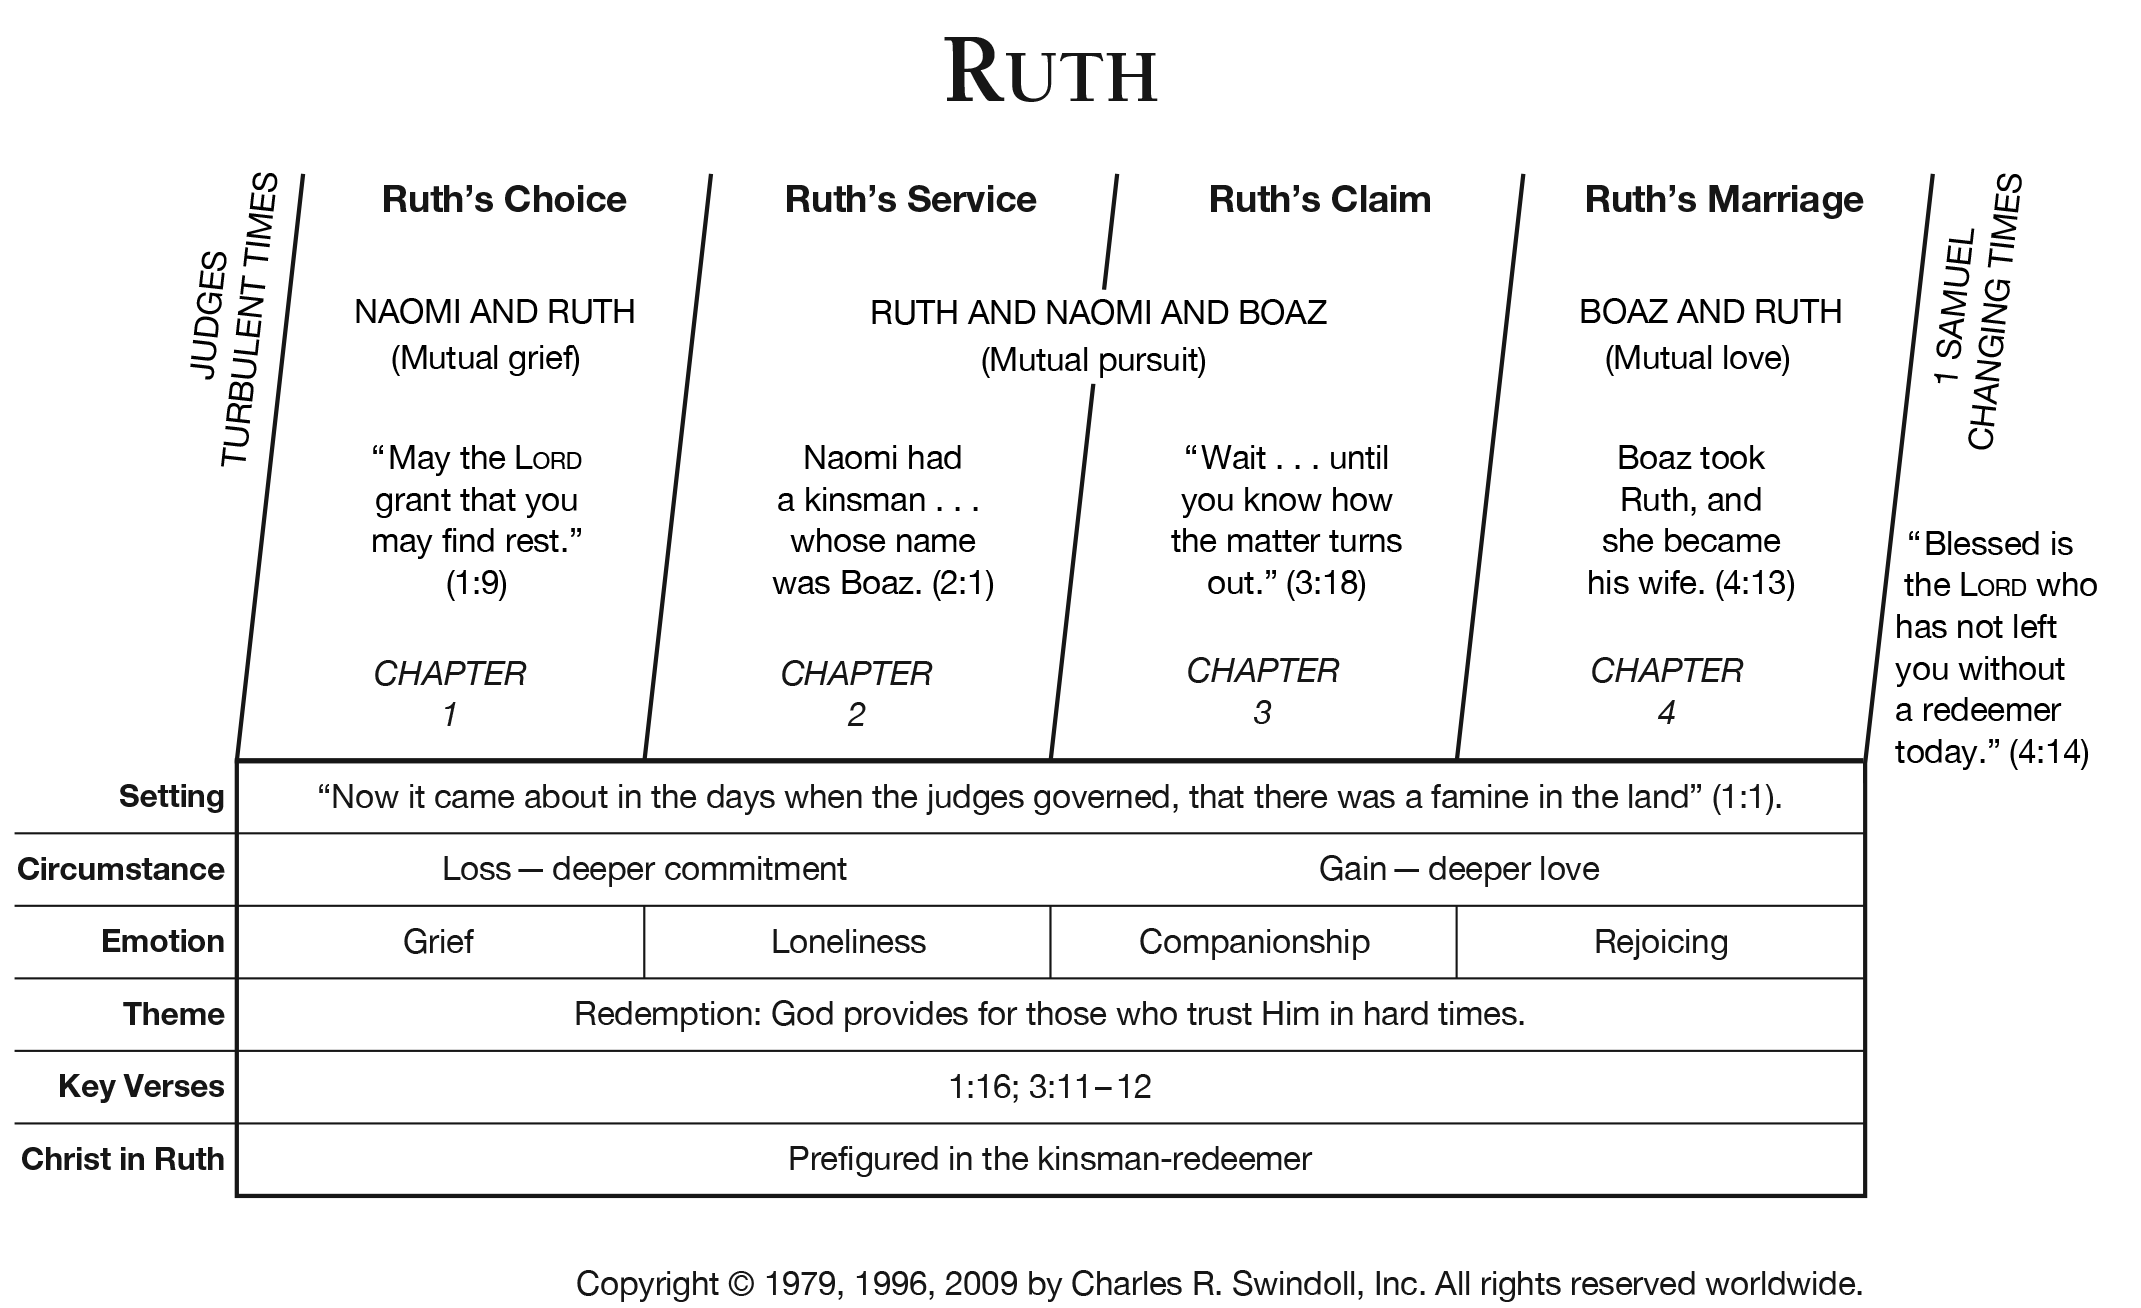
\includegraphics[scale=0.25, angle=90]{08OT-Ruth/References/Swindoll-Ruth}
\caption[Ruth from Swindoll]{Ruth from The Swindoll}
\label{fig:Ruth from Swindoll}
\end{center}
\end{figure}

\newpage
\begin{figure}
\begin{center}
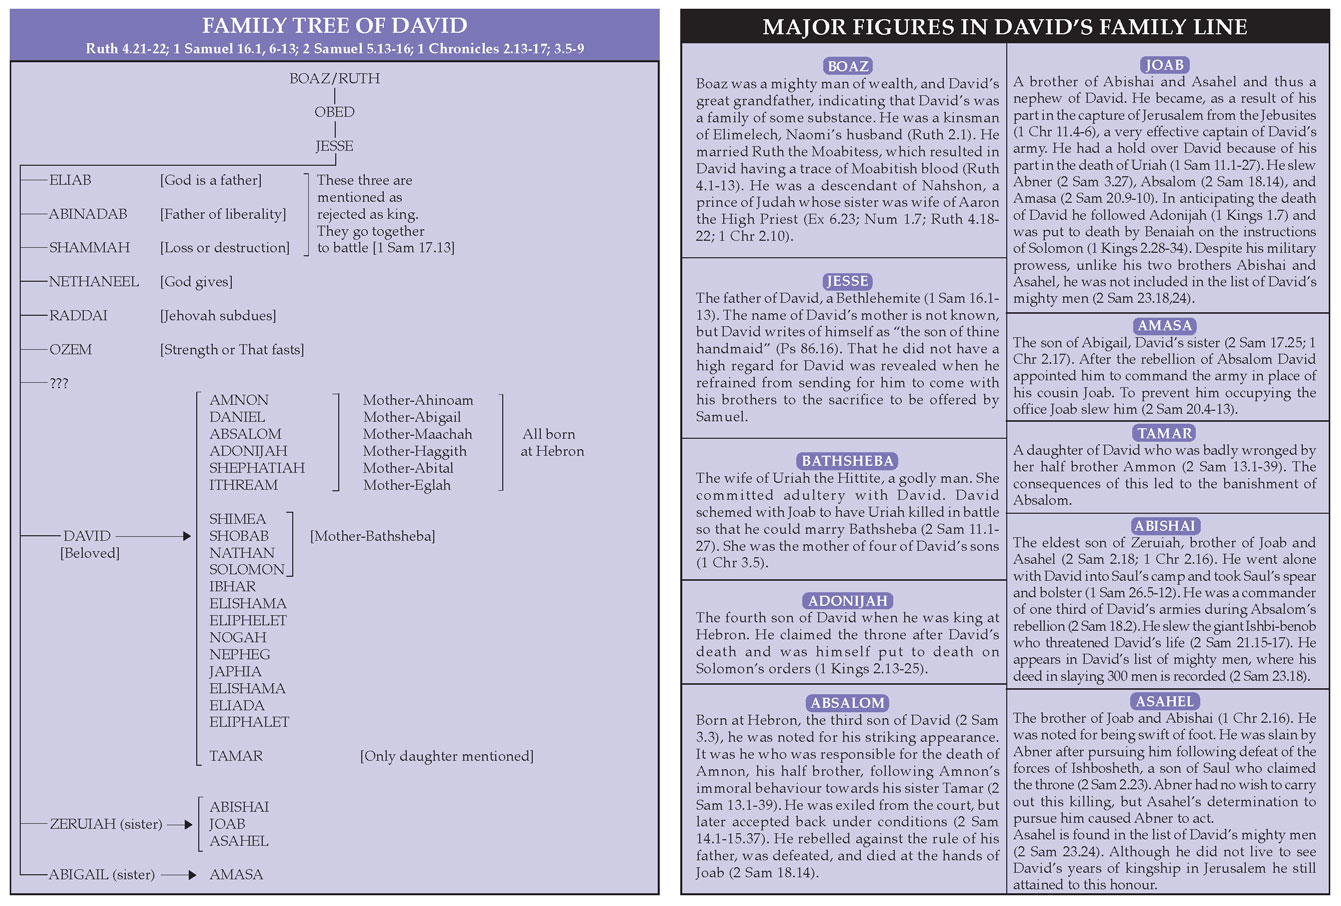
\includegraphics[scale=0.4, angle=90]{08OT-Ruth/References/JohnGrantFamilyTreeOfDavid}
\caption[The Family Tree of David]{The Family Tree of David}
\label{fig:The Family Tree of David}
\end{center}
\end{figure}


\chapter{Ruth 1}


\marginpar{\scriptsize \centering \fcolorbox{bone}{lime}{\textbf{COMING BACK BROKEN}}\\ (Ruth 1:1-22) \begin{compactenum}[I.][8]
    \item The \textbf{Longing} (for Food) \index[scripture]{Ruth!Ruth 01:01}(Ruth 1:1)
    \item The \textbf{Looking} (at Moab) \index[scripture]{Ruth!Ruth 01:01}(Ruth 1:1)
    \item The \textbf{Leaving} (the land of faith for the land of the flesh) \index[scripture]{Ruth!Ruth 01:01}(Ruth 1:1)
    \item The \textbf{Loosing} (husband and sons) \index[scripture]{Ruth!Ruth 01:03}\index[scripture]{Ruth!Ruth 01:05}(Ruth 1:3, 5)
    \item The \textbf{Learning} (why did she have to suffer loss to know she was in the wrong place?) 
    \item The \textbf{Listening} (why was this a surprise to her?)  \index[scripture]{Ruth!Ruth 01:06}(Ruth 1:6)
    \item Ruth's \textbf{Oblivion} (Naomi was oblivious to Ruth's faith)  %\index[scripture]{Ruth!Ruth 01:06}(Ruth 1:6)
\end{compactenum}}




\footnote{\textcolor[cmyk]{0.99998,1,0,0}{\hyperlink{TOC}{Return to end of Table of Contents.}}}\footnote{\href{https://audiobible.com/bible/ruth_1.html}{\textcolor[cmyk]{0.99998,1,0,0}{Ruth 1 Audio}}}\textcolor[cmyk]{0.99998,1,0,0}{Now it came to pass in the days when the judges ruled, that there was a \fcolorbox{bone}{lime}{famine} in the land. And a certain man of Beth-lehem-judah \fcolorbox{bone}{lime}{went} to sojourn in the country of Moab, he, and his wife, and his two sons.}
[2] \textcolor[cmyk]{0.99998,1,0,0}{And the name of the man \emph{was} Elimelech, and the name of his wife Naomi, and the name of his two sons Mahlon and Chilion, Ephrathites of Beth-lehem-judah. And they came into the country of Moab, and continued there.}
[3] \textcolor[cmyk]{0.99998,1,0,0}{And Elimelech Naomi's \fcolorbox{bone}{lime}{husband died}; and she was left, and her two sons.}
[4] \textcolor[cmyk]{0.99998,1,0,0}{And they took them wives of the women of Moab; the name of the one \emph{was} Orpah, and the name of the other Ruth: and they dwelled there about ten years.}
[5] \textcolor[cmyk]{0.99998,1,0,0}{And \fcolorbox{bone}{lime}{Mahlon and Chilion} died also both of them; and the woman was left of her two sons and her husband.}\\
\\
\P \textcolor[cmyk]{0.99998,1,0,0}{Then she arose with her daughters in law, that she might return from the country of Moab: for she had \fcolorbox{bone}{lime}{heard} in the country of Moab how that the LORD had visited his people in giving them bread.}
[7] \textcolor[cmyk]{0.99998,1,0,0}{Wherefore she went forth out of the place where she was, and her two daughters in law with her; and they went on the way to return unto the land of Judah.}
[8] \textcolor[cmyk]{0.99998,1,0,0}{And Naomi said unto her two daughters in law, Go, return each to her mother's house: the LORD deal kindly with you, as ye have dealt with the dead, and with me.}
[9] \textcolor[cmyk]{0.99998,1,0,0}{The LORD grant you that ye may find rest, each \emph{of} \emph{you} in the house of her husband. Then she kissed them; and they lifted up their voice, and wept.}
[10] \textcolor[cmyk]{0.99998,1,0,0}{And they said unto her, Surely we will return with thee unto thy people.}
[11] \textcolor[cmyk]{0.99998,1,0,0}{And Naomi said, Turn again, my daughters: why will ye go with me? \emph{are} there yet \emph{any} \emph{more} sons in my womb, that they may be your husbands?}
[12] \textcolor[cmyk]{0.99998,1,0,0}{Turn again, my daughters, go \emph{your} \emph{way}; for I am too old to have an husband. If I should say, I have hope, \emph{if} I should have an husband also to night, and should also bear sons;}
[13] \textcolor[cmyk]{0.99998,1,0,0}{Would ye tarry for them till they were grown? would ye stay for them from having husbands? nay, my daughters; for it grieveth me much for your sakes that the hand of the LORD is gone out against me.}
[14] \textcolor[cmyk]{0.99998,1,0,0}{And they lifted up their voice, and wept again: and Orpah kissed her mother in law; but Ruth clave unto her.}
[15] \textcolor[cmyk]{0.99998,1,0,0}{And she said, Behold, thy sister in law is gone back unto her people, and unto her gods: return thou after thy sister in law.}
[16] \textcolor[cmyk]{0.99998,1,0,0}{And Ruth said, Intreat me not to leave thee, \emph{or} to return from following after thee: for whither thou goest, I will go; and where thou lodgest, I will lodge: thy people \emph{shall} \emph{be} my people, and thy God my God:}
[17] \textcolor[cmyk]{0.99998,1,0,0}{Where thou diest, will I die, and there will I be buried: the LORD do so to me, and more also, \emph{if} \emph{ought} but death part thee and me.}
[18] \textcolor[cmyk]{0.99998,1,0,0}{When she saw that she was stedfastly minded to go with her, then she left speaking unto her.}
[19] \textcolor[cmyk]{0.99998,1,0,0}{So they two went until they came to Beth-lehem. And it came to pass, when they were come to Beth-lehem, that all the city was moved about them, and they said, \emph{Is} this Naomi?}
[20] \textcolor[cmyk]{0.99998,1,0,0}{And she said unto them, Call me not Naomi, call me Mara: for the Almighty hath dealt very bitterly with me.}
[21] \textcolor[cmyk]{0.99998,1,0,0}{I went out full, and the LORD hath brought me home again empty: why \emph{then} call ye me Naomi, seeing the LORD hath testified against me, and the Almighty hath afflicted me?}
[22] \textcolor[cmyk]{0.99998,1,0,0}{So Naomi returned, and Ruth the Moabitess, her daughter in law, with her, which returned out of the country of Moab: and they came to Beth-lehem in the beginning of barley harvest.}

\index[NWIV]{42!Ruth!Rut 1:1}\index[AWIP]{Now!Ruth!Rut 1:1}\index[AWIP]{it!Ruth!Rut 1:1}\index[AWIP]{came!Ruth!Rut 1:1}\index[AWIP]{to!Ruth!Rut 1:1}\index[AWIP]{to!Ruth!Rut 1:1 (2)}\index[AWIP]{pass!Ruth!Rut 1:1}\index[AWIP]{in!Ruth!Rut 1:1}\index[AWIP]{in!Ruth!Rut 1:1 (2)}\index[AWIP]{in!Ruth!Rut 1:1 (3)}\index[AWIP]{the!Ruth!Rut 1:1}\index[AWIP]{the!Ruth!Rut 1:1 (2)}\index[AWIP]{the!Ruth!Rut 1:1 (3)}\index[AWIP]{the!Ruth!Rut 1:1 (4)}\index[AWIP]{days!Ruth!Rut 1:1}\index[AWIP]{when!Ruth!Rut 1:1}\index[AWIP]{judges!Ruth!Rut 1:1}\index[AWIP]{ruled!Ruth!Rut 1:1}\index[AWIP]{that!Ruth!Rut 1:1}\index[AWIP]{there!Ruth!Rut 1:1}\index[AWIP]{was!Ruth!Rut 1:1}\index[AWIP]{a!Ruth!Rut 1:1}\index[AWIP]{a!Ruth!Rut 1:1 (2)}\index[AWIP]{famine!Ruth!Rut 1:1}\index[AWIP]{land!Ruth!Rut 1:1}\index[AWIP]{And!Ruth!Rut 1:1}\index[AWIP]{certain!Ruth!Rut 1:1}\index[AWIP]{man!Ruth!Rut 1:1}\index[AWIP]{of!Ruth!Rut 1:1}\index[AWIP]{of!Ruth!Rut 1:1 (2)}\index[AWIP]{Beth-lehem-judah!Ruth!Rut 1:1}\index[AWIP]{went!Ruth!Rut 1:1}\index[AWIP]{sojourn!Ruth!Rut 1:1}\index[AWIP]{country!Ruth!Rut 1:1}\index[AWIP]{Moab!Ruth!Rut 1:1}\index[AWIP]{he!Ruth!Rut 1:1}\index[AWIP]{and!Ruth!Rut 1:1}\index[AWIP]{and!Ruth!Rut 1:1 (2)}\index[AWIP]{his!Ruth!Rut 1:1}\index[AWIP]{his!Ruth!Rut 1:1 (2)}\index[AWIP]{wife!Ruth!Rut 1:1}\index[AWIP]{two!Ruth!Rut 1:1}\index[AWIP]{sons!Ruth!Rut 1:1}

\index[NWIV]{39!Ruth!Rut 1:2}\index[AWIP]{And!Ruth!Rut 1:2}\index[AWIP]{And!Ruth!Rut 1:2 (2)}\index[AWIP]{the!Ruth!Rut 1:2}\index[AWIP]{the!Ruth!Rut 1:2 (2)}\index[AWIP]{the!Ruth!Rut 1:2 (3)}\index[AWIP]{the!Ruth!Rut 1:2 (4)}\index[AWIP]{the!Ruth!Rut 1:2 (5)}\index[AWIP]{name!Ruth!Rut 1:2}\index[AWIP]{name!Ruth!Rut 1:2 (2)}\index[AWIP]{name!Ruth!Rut 1:2 (3)}\index[AWIP]{of!Ruth!Rut 1:2}\index[AWIP]{of!Ruth!Rut 1:2 (2)}\index[AWIP]{of!Ruth!Rut 1:2 (3)}\index[AWIP]{of!Ruth!Rut 1:2 (4)}\index[AWIP]{of!Ruth!Rut 1:2 (5)}\index[AWIP]{man!Ruth!Rut 1:2}\index[AWIP]{\emph{was}!Ruth!Rut 1:2}\index[AWIP]{Elimelech!Ruth!Rut 1:2}\index[AWIP]{and!Ruth!Rut 1:2}\index[AWIP]{and!Ruth!Rut 1:2 (2)}\index[AWIP]{and!Ruth!Rut 1:2 (3)}\index[AWIP]{and!Ruth!Rut 1:2 (4)}\index[AWIP]{his!Ruth!Rut 1:2}\index[AWIP]{his!Ruth!Rut 1:2 (2)}\index[AWIP]{wife!Ruth!Rut 1:2}\index[AWIP]{Naomi!Ruth!Rut 1:2}\index[AWIP]{two!Ruth!Rut 1:2}\index[AWIP]{sons!Ruth!Rut 1:2}\index[AWIP]{Mahlon!Ruth!Rut 1:2}\index[AWIP]{Chilion!Ruth!Rut 1:2}\index[AWIP]{Ephrathites!Ruth!Rut 1:2}\index[AWIP]{Beth-lehem-judah!Ruth!Rut 1:2}\index[AWIP]{they!Ruth!Rut 1:2}\index[AWIP]{came!Ruth!Rut 1:2}\index[AWIP]{into!Ruth!Rut 1:2}\index[AWIP]{country!Ruth!Rut 1:2}\index[AWIP]{Moab!Ruth!Rut 1:2}\index[AWIP]{continued!Ruth!Rut 1:2}\index[AWIP]{there!Ruth!Rut 1:2}\index[AWIP]{\emph{was}!Ruth!Rut 1:2}

\index[NWIV]{13!Ruth!Rut 1:3}\index[AWIP]{And!Ruth!Rut 1:3}\index[AWIP]{Elimelech!Ruth!Rut 1:3}\index[AWIP]{Naomi's!Ruth!Rut 1:3}\index[AWIP]{husband!Ruth!Rut 1:3}\index[AWIP]{died!Ruth!Rut 1:3}\index[AWIP]{and!Ruth!Rut 1:3}\index[AWIP]{and!Ruth!Rut 1:3 (2)}\index[AWIP]{she!Ruth!Rut 1:3}\index[AWIP]{was!Ruth!Rut 1:3}\index[AWIP]{left!Ruth!Rut 1:3}\index[AWIP]{her!Ruth!Rut 1:3}\index[AWIP]{two!Ruth!Rut 1:3}\index[AWIP]{sons!Ruth!Rut 1:3}

\index[NWIV]{31!Ruth!Rut 1:4}\index[AWIP]{And!Ruth!Rut 1:4}\index[AWIP]{they!Ruth!Rut 1:4}\index[AWIP]{they!Ruth!Rut 1:4 (2)}\index[AWIP]{took!Ruth!Rut 1:4}\index[AWIP]{them!Ruth!Rut 1:4}\index[AWIP]{wives!Ruth!Rut 1:4}\index[AWIP]{of!Ruth!Rut 1:4}\index[AWIP]{of!Ruth!Rut 1:4 (2)}\index[AWIP]{of!Ruth!Rut 1:4 (3)}\index[AWIP]{of!Ruth!Rut 1:4 (4)}\index[AWIP]{the!Ruth!Rut 1:4}\index[AWIP]{the!Ruth!Rut 1:4 (2)}\index[AWIP]{the!Ruth!Rut 1:4 (3)}\index[AWIP]{the!Ruth!Rut 1:4 (4)}\index[AWIP]{the!Ruth!Rut 1:4 (5)}\index[AWIP]{women!Ruth!Rut 1:4}\index[AWIP]{Moab!Ruth!Rut 1:4}\index[AWIP]{name!Ruth!Rut 1:4}\index[AWIP]{name!Ruth!Rut 1:4 (2)}\index[AWIP]{one!Ruth!Rut 1:4}\index[AWIP]{\emph{was}!Ruth!Rut 1:4}\index[AWIP]{Orpah!Ruth!Rut 1:4}\index[AWIP]{and!Ruth!Rut 1:4}\index[AWIP]{and!Ruth!Rut 1:4 (2)}\index[AWIP]{other!Ruth!Rut 1:4}\index[AWIP]{Ruth!Ruth!Rut 1:4}\index[AWIP]{dwelled!Ruth!Rut 1:4}\index[AWIP]{there!Ruth!Rut 1:4}\index[AWIP]{about!Ruth!Rut 1:4}\index[AWIP]{ten!Ruth!Rut 1:4}\index[AWIP]{years!Ruth!Rut 1:4}\index[AWIP]{\emph{was}!Ruth!Rut 1:4}

\index[NWIV]{21!Ruth!Rut 1:5}\index[AWIP]{And!Ruth!Rut 1:5}\index[AWIP]{Mahlon!Ruth!Rut 1:5}\index[AWIP]{and!Ruth!Rut 1:5}\index[AWIP]{and!Ruth!Rut 1:5 (2)}\index[AWIP]{and!Ruth!Rut 1:5 (3)}\index[AWIP]{Chilion!Ruth!Rut 1:5}\index[AWIP]{died!Ruth!Rut 1:5}\index[AWIP]{also!Ruth!Rut 1:5}\index[AWIP]{both!Ruth!Rut 1:5}\index[AWIP]{of!Ruth!Rut 1:5}\index[AWIP]{of!Ruth!Rut 1:5 (2)}\index[AWIP]{them!Ruth!Rut 1:5}\index[AWIP]{the!Ruth!Rut 1:5}\index[AWIP]{woman!Ruth!Rut 1:5}\index[AWIP]{was!Ruth!Rut 1:5}\index[AWIP]{left!Ruth!Rut 1:5}\index[AWIP]{her!Ruth!Rut 1:5}\index[AWIP]{her!Ruth!Rut 1:5 (2)}\index[AWIP]{two!Ruth!Rut 1:5}\index[AWIP]{sons!Ruth!Rut 1:5}\index[AWIP]{husband!Ruth!Rut 1:5}

\index[NWIV]{38!Ruth!Rut 1:6}\index[AWIP]{Then!Ruth!Rut 1:6}\index[AWIP]{she!Ruth!Rut 1:6}\index[AWIP]{she!Ruth!Rut 1:6 (2)}\index[AWIP]{she!Ruth!Rut 1:6 (3)}\index[AWIP]{arose!Ruth!Rut 1:6}\index[AWIP]{with!Ruth!Rut 1:6}\index[AWIP]{her!Ruth!Rut 1:6}\index[AWIP]{daughters!Ruth!Rut 1:6}\index[AWIP]{in!Ruth!Rut 1:6}\index[AWIP]{in!Ruth!Rut 1:6 (2)}\index[AWIP]{in!Ruth!Rut 1:6 (3)}\index[AWIP]{law!Ruth!Rut 1:6}\index[AWIP]{that!Ruth!Rut 1:6}\index[AWIP]{that!Ruth!Rut 1:6 (2)}\index[AWIP]{might!Ruth!Rut 1:6}\index[AWIP]{return!Ruth!Rut 1:6}\index[AWIP]{from!Ruth!Rut 1:6}\index[AWIP]{the!Ruth!Rut 1:6}\index[AWIP]{the!Ruth!Rut 1:6 (2)}\index[AWIP]{the!Ruth!Rut 1:6 (3)}\index[AWIP]{country!Ruth!Rut 1:6}\index[AWIP]{country!Ruth!Rut 1:6 (2)}\index[AWIP]{of!Ruth!Rut 1:6}\index[AWIP]{of!Ruth!Rut 1:6 (2)}\index[AWIP]{Moab!Ruth!Rut 1:6}\index[AWIP]{Moab!Ruth!Rut 1:6 (2)}\index[AWIP]{for!Ruth!Rut 1:6}\index[AWIP]{had!Ruth!Rut 1:6}\index[AWIP]{had!Ruth!Rut 1:6 (2)}\index[AWIP]{heard!Ruth!Rut 1:6}\index[AWIP]{how!Ruth!Rut 1:6}\index[AWIP]{LORD!Ruth!Rut 1:6}\index[AWIP]{visited!Ruth!Rut 1:6}\index[AWIP]{his!Ruth!Rut 1:6}\index[AWIP]{people!Ruth!Rut 1:6}\index[AWIP]{giving!Ruth!Rut 1:6}\index[AWIP]{them!Ruth!Rut 1:6}\index[AWIP]{bread!Ruth!Rut 1:6}

\index[NWIV]{32!Ruth!Rut 1:7}\index[AWIP]{Wherefore!Ruth!Rut 1:7}\index[AWIP]{she!Ruth!Rut 1:7}\index[AWIP]{she!Ruth!Rut 1:7 (2)}\index[AWIP]{went!Ruth!Rut 1:7}\index[AWIP]{went!Ruth!Rut 1:7 (2)}\index[AWIP]{forth!Ruth!Rut 1:7}\index[AWIP]{out!Ruth!Rut 1:7}\index[AWIP]{of!Ruth!Rut 1:7}\index[AWIP]{of!Ruth!Rut 1:7 (2)}\index[AWIP]{the!Ruth!Rut 1:7}\index[AWIP]{the!Ruth!Rut 1:7 (2)}\index[AWIP]{the!Ruth!Rut 1:7 (3)}\index[AWIP]{place!Ruth!Rut 1:7}\index[AWIP]{where!Ruth!Rut 1:7}\index[AWIP]{was!Ruth!Rut 1:7}\index[AWIP]{and!Ruth!Rut 1:7}\index[AWIP]{and!Ruth!Rut 1:7 (2)}\index[AWIP]{her!Ruth!Rut 1:7}\index[AWIP]{her!Ruth!Rut 1:7 (2)}\index[AWIP]{two!Ruth!Rut 1:7}\index[AWIP]{daughters!Ruth!Rut 1:7}\index[AWIP]{in!Ruth!Rut 1:7}\index[AWIP]{law!Ruth!Rut 1:7}\index[AWIP]{with!Ruth!Rut 1:7}\index[AWIP]{they!Ruth!Rut 1:7}\index[AWIP]{on!Ruth!Rut 1:7}\index[AWIP]{way!Ruth!Rut 1:7}\index[AWIP]{to!Ruth!Rut 1:7}\index[AWIP]{return!Ruth!Rut 1:7}\index[AWIP]{unto!Ruth!Rut 1:7}\index[AWIP]{land!Ruth!Rut 1:7}\index[AWIP]{Judah!Ruth!Rut 1:7}

\index[NWIV]{32!Ruth!Rut 1:8}\index[AWIP]{And!Ruth!Rut 1:8}\index[AWIP]{Naomi!Ruth!Rut 1:8}\index[AWIP]{said!Ruth!Rut 1:8}\index[AWIP]{unto!Ruth!Rut 1:8}\index[AWIP]{her!Ruth!Rut 1:8}\index[AWIP]{her!Ruth!Rut 1:8 (2)}\index[AWIP]{two!Ruth!Rut 1:8}\index[AWIP]{daughters!Ruth!Rut 1:8}\index[AWIP]{in!Ruth!Rut 1:8}\index[AWIP]{law!Ruth!Rut 1:8}\index[AWIP]{Go!Ruth!Rut 1:8}\index[AWIP]{return!Ruth!Rut 1:8}\index[AWIP]{each!Ruth!Rut 1:8}\index[AWIP]{to!Ruth!Rut 1:8}\index[AWIP]{mother's!Ruth!Rut 1:8}\index[AWIP]{house!Ruth!Rut 1:8}\index[AWIP]{the!Ruth!Rut 1:8}\index[AWIP]{the!Ruth!Rut 1:8 (2)}\index[AWIP]{LORD!Ruth!Rut 1:8}\index[AWIP]{deal!Ruth!Rut 1:8}\index[AWIP]{kindly!Ruth!Rut 1:8}\index[AWIP]{with!Ruth!Rut 1:8}\index[AWIP]{with!Ruth!Rut 1:8 (2)}\index[AWIP]{with!Ruth!Rut 1:8 (3)}\index[AWIP]{you!Ruth!Rut 1:8}\index[AWIP]{as!Ruth!Rut 1:8}\index[AWIP]{ye!Ruth!Rut 1:8}\index[AWIP]{have!Ruth!Rut 1:8}\index[AWIP]{dealt!Ruth!Rut 1:8}\index[AWIP]{dead!Ruth!Rut 1:8}\index[AWIP]{and!Ruth!Rut 1:8}\index[AWIP]{me!Ruth!Rut 1:8}

\index[NWIV]{30!Ruth!Rut 1:9}\index[AWIP]{The!Ruth!Rut 1:9}\index[AWIP]{LORD!Ruth!Rut 1:9}\index[AWIP]{grant!Ruth!Rut 1:9}\index[AWIP]{you!Ruth!Rut 1:9}\index[AWIP]{that!Ruth!Rut 1:9}\index[AWIP]{ye!Ruth!Rut 1:9}\index[AWIP]{may!Ruth!Rut 1:9}\index[AWIP]{find!Ruth!Rut 1:9}\index[AWIP]{rest!Ruth!Rut 1:9}\index[AWIP]{each!Ruth!Rut 1:9}\index[AWIP]{\emph{of}!Ruth!Rut 1:9}\index[AWIP]{\emph{you}!Ruth!Rut 1:9}\index[AWIP]{in!Ruth!Rut 1:9}\index[AWIP]{the!Ruth!Rut 1:9}\index[AWIP]{house!Ruth!Rut 1:9}\index[AWIP]{of!Ruth!Rut 1:9}\index[AWIP]{her!Ruth!Rut 1:9}\index[AWIP]{husband!Ruth!Rut 1:9}\index[AWIP]{Then!Ruth!Rut 1:9}\index[AWIP]{she!Ruth!Rut 1:9}\index[AWIP]{kissed!Ruth!Rut 1:9}\index[AWIP]{them!Ruth!Rut 1:9}\index[AWIP]{and!Ruth!Rut 1:9}\index[AWIP]{and!Ruth!Rut 1:9 (2)}\index[AWIP]{they!Ruth!Rut 1:9}\index[AWIP]{lifted!Ruth!Rut 1:9}\index[AWIP]{up!Ruth!Rut 1:9}\index[AWIP]{their!Ruth!Rut 1:9}\index[AWIP]{voice!Ruth!Rut 1:9}\index[AWIP]{wept!Ruth!Rut 1:9}\index[AWIP]{\emph{of}!Ruth!Rut 1:9}\index[AWIP]{\emph{you}!Ruth!Rut 1:9}

\index[NWIV]{14!Ruth!Rut 1:10}\index[AWIP]{And!Ruth!Rut 1:10}\index[AWIP]{they!Ruth!Rut 1:10}\index[AWIP]{said!Ruth!Rut 1:10}\index[AWIP]{unto!Ruth!Rut 1:10}\index[AWIP]{unto!Ruth!Rut 1:10 (2)}\index[AWIP]{her!Ruth!Rut 1:10}\index[AWIP]{Surely!Ruth!Rut 1:10}\index[AWIP]{we!Ruth!Rut 1:10}\index[AWIP]{will!Ruth!Rut 1:10}\index[AWIP]{return!Ruth!Rut 1:10}\index[AWIP]{with!Ruth!Rut 1:10}\index[AWIP]{thee!Ruth!Rut 1:10}\index[AWIP]{thy!Ruth!Rut 1:10}\index[AWIP]{people!Ruth!Rut 1:10}

\index[NWIV]{28!Ruth!Rut 1:11}\index[AWIP]{And!Ruth!Rut 1:11}\index[AWIP]{Naomi!Ruth!Rut 1:11}\index[AWIP]{said!Ruth!Rut 1:11}\index[AWIP]{Turn!Ruth!Rut 1:11}\index[AWIP]{again!Ruth!Rut 1:11}\index[AWIP]{my!Ruth!Rut 1:11}\index[AWIP]{my!Ruth!Rut 1:11 (2)}\index[AWIP]{daughters!Ruth!Rut 1:11}\index[AWIP]{why!Ruth!Rut 1:11}\index[AWIP]{will!Ruth!Rut 1:11}\index[AWIP]{ye!Ruth!Rut 1:11}\index[AWIP]{go!Ruth!Rut 1:11}\index[AWIP]{with!Ruth!Rut 1:11}\index[AWIP]{me?!Ruth!Rut 1:11}\index[AWIP]{\emph{are}!Ruth!Rut 1:11}\index[AWIP]{there!Ruth!Rut 1:11}\index[AWIP]{yet!Ruth!Rut 1:11}\index[AWIP]{\emph{any}!Ruth!Rut 1:11}\index[AWIP]{\emph{more}!Ruth!Rut 1:11}\index[AWIP]{sons!Ruth!Rut 1:11}\index[AWIP]{in!Ruth!Rut 1:11}\index[AWIP]{womb!Ruth!Rut 1:11}\index[AWIP]{that!Ruth!Rut 1:11}\index[AWIP]{they!Ruth!Rut 1:11}\index[AWIP]{may!Ruth!Rut 1:11}\index[AWIP]{be!Ruth!Rut 1:11}\index[AWIP]{your!Ruth!Rut 1:11}\index[AWIP]{husbands?!Ruth!Rut 1:11}\index[AWIP]{\emph{are}!Ruth!Rut 1:11}\index[AWIP]{\emph{any}!Ruth!Rut 1:11}\index[AWIP]{\emph{more}!Ruth!Rut 1:11}

\index[NWIV]{37!Ruth!Rut 1:12}\index[AWIP]{Turn!Ruth!Rut 1:12}\index[AWIP]{again!Ruth!Rut 1:12}\index[AWIP]{my!Ruth!Rut 1:12}\index[AWIP]{daughters!Ruth!Rut 1:12}\index[AWIP]{go!Ruth!Rut 1:12}\index[AWIP]{\emph{your}!Ruth!Rut 1:12}\index[AWIP]{\emph{way}!Ruth!Rut 1:12}\index[AWIP]{for!Ruth!Rut 1:12}\index[AWIP]{I!Ruth!Rut 1:12}\index[AWIP]{I!Ruth!Rut 1:12 (2)}\index[AWIP]{I!Ruth!Rut 1:12 (3)}\index[AWIP]{I!Ruth!Rut 1:12 (4)}\index[AWIP]{am!Ruth!Rut 1:12}\index[AWIP]{too!Ruth!Rut 1:12}\index[AWIP]{old!Ruth!Rut 1:12}\index[AWIP]{to!Ruth!Rut 1:12}\index[AWIP]{to!Ruth!Rut 1:12 (2)}\index[AWIP]{have!Ruth!Rut 1:12}\index[AWIP]{have!Ruth!Rut 1:12 (2)}\index[AWIP]{have!Ruth!Rut 1:12 (3)}\index[AWIP]{an!Ruth!Rut 1:12}\index[AWIP]{an!Ruth!Rut 1:12 (2)}\index[AWIP]{husband!Ruth!Rut 1:12}\index[AWIP]{husband!Ruth!Rut 1:12 (2)}\index[AWIP]{If!Ruth!Rut 1:12}\index[AWIP]{should!Ruth!Rut 1:12}\index[AWIP]{should!Ruth!Rut 1:12 (2)}\index[AWIP]{should!Ruth!Rut 1:12 (3)}\index[AWIP]{say!Ruth!Rut 1:12}\index[AWIP]{hope!Ruth!Rut 1:12}\index[AWIP]{\emph{if}!Ruth!Rut 1:12}\index[AWIP]{also!Ruth!Rut 1:12}\index[AWIP]{also!Ruth!Rut 1:12 (2)}\index[AWIP]{night!Ruth!Rut 1:12}\index[AWIP]{and!Ruth!Rut 1:12}\index[AWIP]{bear!Ruth!Rut 1:12}\index[AWIP]{sons!Ruth!Rut 1:12}\index[AWIP]{\emph{your}!Ruth!Rut 1:12}\index[AWIP]{\emph{way}!Ruth!Rut 1:12}\index[AWIP]{\emph{if}!Ruth!Rut 1:12}

\index[NWIV]{39!Ruth!Rut 1:13}\index[AWIP]{Would!Ruth!Rut 1:13}\index[AWIP]{ye!Ruth!Rut 1:13}\index[AWIP]{ye!Ruth!Rut 1:13 (2)}\index[AWIP]{tarry!Ruth!Rut 1:13}\index[AWIP]{for!Ruth!Rut 1:13}\index[AWIP]{for!Ruth!Rut 1:13 (2)}\index[AWIP]{for!Ruth!Rut 1:13 (3)}\index[AWIP]{for!Ruth!Rut 1:13 (4)}\index[AWIP]{them!Ruth!Rut 1:13}\index[AWIP]{them!Ruth!Rut 1:13 (2)}\index[AWIP]{till!Ruth!Rut 1:13}\index[AWIP]{they!Ruth!Rut 1:13}\index[AWIP]{were!Ruth!Rut 1:13}\index[AWIP]{grown?!Ruth!Rut 1:13}\index[AWIP]{would!Ruth!Rut 1:13}\index[AWIP]{stay!Ruth!Rut 1:13}\index[AWIP]{from!Ruth!Rut 1:13}\index[AWIP]{having!Ruth!Rut 1:13}\index[AWIP]{husbands?!Ruth!Rut 1:13}\index[AWIP]{nay!Ruth!Rut 1:13}\index[AWIP]{my!Ruth!Rut 1:13}\index[AWIP]{daughters!Ruth!Rut 1:13}\index[AWIP]{it!Ruth!Rut 1:13}\index[AWIP]{grieveth!Ruth!Rut 1:13}\index[AWIP]{me!Ruth!Rut 1:13}\index[AWIP]{me!Ruth!Rut 1:13 (2)}\index[AWIP]{much!Ruth!Rut 1:13}\index[AWIP]{your!Ruth!Rut 1:13}\index[AWIP]{sakes!Ruth!Rut 1:13}\index[AWIP]{that!Ruth!Rut 1:13}\index[AWIP]{the!Ruth!Rut 1:13}\index[AWIP]{the!Ruth!Rut 1:13 (2)}\index[AWIP]{hand!Ruth!Rut 1:13}\index[AWIP]{of!Ruth!Rut 1:13}\index[AWIP]{LORD!Ruth!Rut 1:13}\index[AWIP]{is!Ruth!Rut 1:13}\index[AWIP]{gone!Ruth!Rut 1:13}\index[AWIP]{out!Ruth!Rut 1:13}\index[AWIP]{against!Ruth!Rut 1:13}

\index[NWIV]{21!Ruth!Rut 1:14}\index[AWIP]{And!Ruth!Rut 1:14}\index[AWIP]{they!Ruth!Rut 1:14}\index[AWIP]{lifted!Ruth!Rut 1:14}\index[AWIP]{up!Ruth!Rut 1:14}\index[AWIP]{their!Ruth!Rut 1:14}\index[AWIP]{voice!Ruth!Rut 1:14}\index[AWIP]{and!Ruth!Rut 1:14}\index[AWIP]{and!Ruth!Rut 1:14 (2)}\index[AWIP]{wept!Ruth!Rut 1:14}\index[AWIP]{again!Ruth!Rut 1:14}\index[AWIP]{Orpah!Ruth!Rut 1:14}\index[AWIP]{kissed!Ruth!Rut 1:14}\index[AWIP]{her!Ruth!Rut 1:14}\index[AWIP]{her!Ruth!Rut 1:14 (2)}\index[AWIP]{mother!Ruth!Rut 1:14}\index[AWIP]{in!Ruth!Rut 1:14}\index[AWIP]{law!Ruth!Rut 1:14}\index[AWIP]{but!Ruth!Rut 1:14}\index[AWIP]{Ruth!Ruth!Rut 1:14}\index[AWIP]{clave!Ruth!Rut 1:14}\index[AWIP]{unto!Ruth!Rut 1:14}

\index[NWIV]{25!Ruth!Rut 1:15}\index[AWIP]{And!Ruth!Rut 1:15}\index[AWIP]{she!Ruth!Rut 1:15}\index[AWIP]{said!Ruth!Rut 1:15}\index[AWIP]{Behold!Ruth!Rut 1:15}\index[AWIP]{thy!Ruth!Rut 1:15}\index[AWIP]{thy!Ruth!Rut 1:15 (2)}\index[AWIP]{sister!Ruth!Rut 1:15}\index[AWIP]{sister!Ruth!Rut 1:15 (2)}\index[AWIP]{in!Ruth!Rut 1:15}\index[AWIP]{in!Ruth!Rut 1:15 (2)}\index[AWIP]{law!Ruth!Rut 1:15}\index[AWIP]{law!Ruth!Rut 1:15 (2)}\index[AWIP]{is!Ruth!Rut 1:15}\index[AWIP]{gone!Ruth!Rut 1:15}\index[AWIP]{back!Ruth!Rut 1:15}\index[AWIP]{unto!Ruth!Rut 1:15}\index[AWIP]{unto!Ruth!Rut 1:15 (2)}\index[AWIP]{her!Ruth!Rut 1:15}\index[AWIP]{her!Ruth!Rut 1:15 (2)}\index[AWIP]{people!Ruth!Rut 1:15}\index[AWIP]{and!Ruth!Rut 1:15}\index[AWIP]{gods!Ruth!Rut 1:15}\index[AWIP]{return!Ruth!Rut 1:15}\index[AWIP]{thou!Ruth!Rut 1:15}\index[AWIP]{after!Ruth!Rut 1:15}

\index[NWIV]{41!Ruth!Rut 1:16}\index[AWIP]{And!Ruth!Rut 1:16}\index[AWIP]{Ruth!Ruth!Rut 1:16}\index[AWIP]{said!Ruth!Rut 1:16}\index[AWIP]{Intreat!Ruth!Rut 1:16}\index[AWIP]{me!Ruth!Rut 1:16}\index[AWIP]{not!Ruth!Rut 1:16}\index[AWIP]{to!Ruth!Rut 1:16}\index[AWIP]{to!Ruth!Rut 1:16 (2)}\index[AWIP]{leave!Ruth!Rut 1:16}\index[AWIP]{thee!Ruth!Rut 1:16}\index[AWIP]{thee!Ruth!Rut 1:16 (2)}\index[AWIP]{\emph{or}!Ruth!Rut 1:16}\index[AWIP]{return!Ruth!Rut 1:16}\index[AWIP]{from!Ruth!Rut 1:16}\index[AWIP]{following!Ruth!Rut 1:16}\index[AWIP]{after!Ruth!Rut 1:16}\index[AWIP]{for!Ruth!Rut 1:16}\index[AWIP]{whither!Ruth!Rut 1:16}\index[AWIP]{thou!Ruth!Rut 1:16}\index[AWIP]{thou!Ruth!Rut 1:16 (2)}\index[AWIP]{goest!Ruth!Rut 1:16}\index[AWIP]{I!Ruth!Rut 1:16}\index[AWIP]{I!Ruth!Rut 1:16 (2)}\index[AWIP]{will!Ruth!Rut 1:16}\index[AWIP]{will!Ruth!Rut 1:16 (2)}\index[AWIP]{go!Ruth!Rut 1:16}\index[AWIP]{and!Ruth!Rut 1:16}\index[AWIP]{and!Ruth!Rut 1:16 (2)}\index[AWIP]{where!Ruth!Rut 1:16}\index[AWIP]{lodgest!Ruth!Rut 1:16}\index[AWIP]{lodge!Ruth!Rut 1:16}\index[AWIP]{thy!Ruth!Rut 1:16}\index[AWIP]{thy!Ruth!Rut 1:16 (2)}\index[AWIP]{people!Ruth!Rut 1:16}\index[AWIP]{people!Ruth!Rut 1:16 (2)}\index[AWIP]{\emph{shall}!Ruth!Rut 1:16}\index[AWIP]{\emph{be}!Ruth!Rut 1:16}\index[AWIP]{my!Ruth!Rut 1:16}\index[AWIP]{my!Ruth!Rut 1:16 (2)}\index[AWIP]{God!Ruth!Rut 1:16}\index[AWIP]{God!Ruth!Rut 1:16 (2)}\index[AWIP]{\emph{or}!Ruth!Rut 1:16}\index[AWIP]{\emph{shall}!Ruth!Rut 1:16}\index[AWIP]{\emph{be}!Ruth!Rut 1:16}

\index[NWIV]{29!Ruth!Rut 1:17}\index[AWIP]{Where!Ruth!Rut 1:17}\index[AWIP]{thou!Ruth!Rut 1:17}\index[AWIP]{diest!Ruth!Rut 1:17}\index[AWIP]{will!Ruth!Rut 1:17}\index[AWIP]{will!Ruth!Rut 1:17 (2)}\index[AWIP]{I!Ruth!Rut 1:17}\index[AWIP]{I!Ruth!Rut 1:17 (2)}\index[AWIP]{die!Ruth!Rut 1:17}\index[AWIP]{and!Ruth!Rut 1:17}\index[AWIP]{and!Ruth!Rut 1:17 (2)}\index[AWIP]{and!Ruth!Rut 1:17 (3)}\index[AWIP]{there!Ruth!Rut 1:17}\index[AWIP]{be!Ruth!Rut 1:17}\index[AWIP]{buried!Ruth!Rut 1:17}\index[AWIP]{the!Ruth!Rut 1:17}\index[AWIP]{LORD!Ruth!Rut 1:17}\index[AWIP]{do!Ruth!Rut 1:17}\index[AWIP]{so!Ruth!Rut 1:17}\index[AWIP]{to!Ruth!Rut 1:17}\index[AWIP]{me!Ruth!Rut 1:17}\index[AWIP]{me!Ruth!Rut 1:17 (2)}\index[AWIP]{more!Ruth!Rut 1:17}\index[AWIP]{also!Ruth!Rut 1:17}\index[AWIP]{\emph{if}!Ruth!Rut 1:17}\index[AWIP]{\emph{ought}!Ruth!Rut 1:17}\index[AWIP]{but!Ruth!Rut 1:17}\index[AWIP]{death!Ruth!Rut 1:17}\index[AWIP]{part!Ruth!Rut 1:17}\index[AWIP]{thee!Ruth!Rut 1:17}\index[AWIP]{\emph{if}!Ruth!Rut 1:17}\index[AWIP]{\emph{ought}!Ruth!Rut 1:17}

\index[NWIV]{18!Ruth!Rut 1:18}\index[AWIP]{When!Ruth!Rut 1:18}\index[AWIP]{she!Ruth!Rut 1:18}\index[AWIP]{she!Ruth!Rut 1:18 (2)}\index[AWIP]{she!Ruth!Rut 1:18 (3)}\index[AWIP]{saw!Ruth!Rut 1:18}\index[AWIP]{that!Ruth!Rut 1:18}\index[AWIP]{was!Ruth!Rut 1:18}\index[AWIP]{stedfastly!Ruth!Rut 1:18}\index[AWIP]{minded!Ruth!Rut 1:18}\index[AWIP]{to!Ruth!Rut 1:18}\index[AWIP]{go!Ruth!Rut 1:18}\index[AWIP]{with!Ruth!Rut 1:18}\index[AWIP]{her!Ruth!Rut 1:18}\index[AWIP]{her!Ruth!Rut 1:18 (2)}\index[AWIP]{then!Ruth!Rut 1:18}\index[AWIP]{left!Ruth!Rut 1:18}\index[AWIP]{speaking!Ruth!Rut 1:18}\index[AWIP]{unto!Ruth!Rut 1:18}

\index[NWIV]{34!Ruth!Rut 1:19}\index[AWIP]{So!Ruth!Rut 1:19}\index[AWIP]{they!Ruth!Rut 1:19}\index[AWIP]{they!Ruth!Rut 1:19 (2)}\index[AWIP]{they!Ruth!Rut 1:19 (3)}\index[AWIP]{they!Ruth!Rut 1:19 (4)}\index[AWIP]{two!Ruth!Rut 1:19}\index[AWIP]{went!Ruth!Rut 1:19}\index[AWIP]{until!Ruth!Rut 1:19}\index[AWIP]{came!Ruth!Rut 1:19}\index[AWIP]{came!Ruth!Rut 1:19 (2)}\index[AWIP]{to!Ruth!Rut 1:19}\index[AWIP]{to!Ruth!Rut 1:19 (2)}\index[AWIP]{to!Ruth!Rut 1:19 (3)}\index[AWIP]{Beth-lehem!Ruth!Rut 1:19}\index[AWIP]{Beth-lehem!Ruth!Rut 1:19 (2)}\index[AWIP]{And!Ruth!Rut 1:19}\index[AWIP]{it!Ruth!Rut 1:19}\index[AWIP]{pass!Ruth!Rut 1:19}\index[AWIP]{when!Ruth!Rut 1:19}\index[AWIP]{were!Ruth!Rut 1:19}\index[AWIP]{come!Ruth!Rut 1:19}\index[AWIP]{that!Ruth!Rut 1:19}\index[AWIP]{all!Ruth!Rut 1:19}\index[AWIP]{the!Ruth!Rut 1:19}\index[AWIP]{city!Ruth!Rut 1:19}\index[AWIP]{was!Ruth!Rut 1:19}\index[AWIP]{moved!Ruth!Rut 1:19}\index[AWIP]{about!Ruth!Rut 1:19}\index[AWIP]{them!Ruth!Rut 1:19}\index[AWIP]{and!Ruth!Rut 1:19}\index[AWIP]{said!Ruth!Rut 1:19}\index[AWIP]{\emph{Is}!Ruth!Rut 1:19}\index[AWIP]{this!Ruth!Rut 1:19}\index[AWIP]{Naomi?!Ruth!Rut 1:19}\index[AWIP]{\emph{Is}!Ruth!Rut 1:19}

\index[NWIV]{21!Ruth!Rut 1:20}\index[AWIP]{And!Ruth!Rut 1:20}\index[AWIP]{she!Ruth!Rut 1:20}\index[AWIP]{said!Ruth!Rut 1:20}\index[AWIP]{unto!Ruth!Rut 1:20}\index[AWIP]{them!Ruth!Rut 1:20}\index[AWIP]{Call!Ruth!Rut 1:20}\index[AWIP]{me!Ruth!Rut 1:20}\index[AWIP]{me!Ruth!Rut 1:20 (2)}\index[AWIP]{me!Ruth!Rut 1:20 (3)}\index[AWIP]{not!Ruth!Rut 1:20}\index[AWIP]{Naomi!Ruth!Rut 1:20}\index[AWIP]{call!Ruth!Rut 1:20}\index[AWIP]{Mara!Ruth!Rut 1:20}\index[AWIP]{for!Ruth!Rut 1:20}\index[AWIP]{the!Ruth!Rut 1:20}\index[AWIP]{Almighty!Ruth!Rut 1:20}\index[AWIP]{hath!Ruth!Rut 1:20}\index[AWIP]{dealt!Ruth!Rut 1:20}\index[AWIP]{very!Ruth!Rut 1:20}\index[AWIP]{bitterly!Ruth!Rut 1:20}\index[AWIP]{with!Ruth!Rut 1:20}

\index[NWIV]{32!Ruth!Rut 1:21}\index[AWIP]{I!Ruth!Rut 1:21}\index[AWIP]{went!Ruth!Rut 1:21}\index[AWIP]{out!Ruth!Rut 1:21}\index[AWIP]{full!Ruth!Rut 1:21}\index[AWIP]{and!Ruth!Rut 1:21}\index[AWIP]{and!Ruth!Rut 1:21 (2)}\index[AWIP]{the!Ruth!Rut 1:21}\index[AWIP]{the!Ruth!Rut 1:21 (2)}\index[AWIP]{the!Ruth!Rut 1:21 (3)}\index[AWIP]{LORD!Ruth!Rut 1:21}\index[AWIP]{LORD!Ruth!Rut 1:21 (2)}\index[AWIP]{hath!Ruth!Rut 1:21}\index[AWIP]{hath!Ruth!Rut 1:21 (2)}\index[AWIP]{hath!Ruth!Rut 1:21 (3)}\index[AWIP]{brought!Ruth!Rut 1:21}\index[AWIP]{me!Ruth!Rut 1:21}\index[AWIP]{me!Ruth!Rut 1:21 (2)}\index[AWIP]{me!Ruth!Rut 1:21 (3)}\index[AWIP]{home!Ruth!Rut 1:21}\index[AWIP]{again!Ruth!Rut 1:21}\index[AWIP]{empty!Ruth!Rut 1:21}\index[AWIP]{why!Ruth!Rut 1:21}\index[AWIP]{\emph{then}!Ruth!Rut 1:21}\index[AWIP]{call!Ruth!Rut 1:21}\index[AWIP]{ye!Ruth!Rut 1:21}\index[AWIP]{Naomi!Ruth!Rut 1:21}\index[AWIP]{seeing!Ruth!Rut 1:21}\index[AWIP]{testified!Ruth!Rut 1:21}\index[AWIP]{against!Ruth!Rut 1:21}\index[AWIP]{Almighty!Ruth!Rut 1:21}\index[AWIP]{afflicted!Ruth!Rut 1:21}\index[AWIP]{me?!Ruth!Rut 1:21}\index[AWIP]{\emph{then}!Ruth!Rut 1:21}

\index[NWIV]{32!Ruth!Rut 1:22}\index[AWIP]{So!Ruth!Rut 1:22}\index[AWIP]{Naomi!Ruth!Rut 1:22}\index[AWIP]{returned!Ruth!Rut 1:22}\index[AWIP]{returned!Ruth!Rut 1:22 (2)}\index[AWIP]{and!Ruth!Rut 1:22}\index[AWIP]{and!Ruth!Rut 1:22 (2)}\index[AWIP]{Ruth!Ruth!Rut 1:22}\index[AWIP]{the!Ruth!Rut 1:22}\index[AWIP]{the!Ruth!Rut 1:22 (2)}\index[AWIP]{the!Ruth!Rut 1:22 (3)}\index[AWIP]{Moabitess!Ruth!Rut 1:22}\index[AWIP]{her!Ruth!Rut 1:22}\index[AWIP]{her!Ruth!Rut 1:22 (2)}\index[AWIP]{daughter!Ruth!Rut 1:22}\index[AWIP]{in!Ruth!Rut 1:22}\index[AWIP]{in!Ruth!Rut 1:22 (2)}\index[AWIP]{law!Ruth!Rut 1:22}\index[AWIP]{with!Ruth!Rut 1:22}\index[AWIP]{which!Ruth!Rut 1:22}\index[AWIP]{out!Ruth!Rut 1:22}\index[AWIP]{of!Ruth!Rut 1:22}\index[AWIP]{of!Ruth!Rut 1:22 (2)}\index[AWIP]{of!Ruth!Rut 1:22 (3)}\index[AWIP]{country!Ruth!Rut 1:22}\index[AWIP]{Moab!Ruth!Rut 1:22}\index[AWIP]{they!Ruth!Rut 1:22}\index[AWIP]{came!Ruth!Rut 1:22}\index[AWIP]{to!Ruth!Rut 1:22}\index[AWIP]{Beth-lehem!Ruth!Rut 1:22}\index[AWIP]{beginning!Ruth!Rut 1:22}\index[AWIP]{barley!Ruth!Rut 1:22}\index[AWIP]{harvest!Ruth!Rut 1:22}


\section{Ruth 1 Outlines}

\subsection{My Outlines}

\subsubsection{Coming Back Broken}
\index[speaker]{Keith Anthony!Ruth 01 (Coming Back Broken)}
\index[series]{Ruth (Keith Anthony)!Ruth 01 (Coming Back Broken)}
\index[date]{2017/03/21!Ruth 01 (Coming Back Broken) (Keith Anthony)}
\textbf{Introduction: }Naomi's return to Bethlehem pictures Israel return back to the land during the church Age. She comes back bitter and broken, but gets blessed by her connection to Ruth and Boaz. Later she gets to witness a wedding between the two!
\begin{compactenum}[I.][7]
    \item The \textbf{Longing} (for food) \index[scripture]{Ruth!Ruth 01:01}(Ruth 1:1)
    \item The \textbf{Looking} (at Moab) \index[scripture]{Ruth!Ruth 01:01}(Ruth 1:1)
    \item The \textbf{Leaving} (the land of faith for the land of the flesh) \index[scripture]{Ruth!Ruth 01:01}(Ruth 1:1)
    \item The \textbf{Loosing} (husband and sons) \index[scripture]{Ruth!Ruth 01:03}\index[scripture]{Ruth!Ruth 01:05}(Ruth 1:3, 5)
    \item The \textbf{Learning} (why did she have to suffer loss to know she was in the wrong place?) 
    \item The \textbf{Listening} (why was this a surprise to her?)  \index[scripture]{Ruth!Ruth 01:06}(Ruth 1:6)
    \item Ruth's \textbf{Oblivion} (Naomi was oblivious to Ruth's faith)  %\index[scripture]{Ruth!Ruth 01:06}(Ruth 1:6)
\end{compactenum}



\subsection{Outlines from Others}

\subsubsection{Three Tombstones in a Washpot}
\index[speaker]{unknown!Ruth 01:01-07 (Three Tombstones in a Washpot)}
\index[series]{Ruth (unknown)!Ruth 01:01-07 (Three Tombstones in a Washpot)}
\index[date]{unknown!Ruth 01:01-07 (Three Tombstones in a Washpot) (unknown)}
\textbf{Source: }sermonnotebook.org\\
\textbf{Introduction: }The little book of Ruth has been called ``the greatest piece of literature ever written.'' Another writer called the story of Ruth ``the Cinderella of the Bible.'' It is the story of how a pagan girl named Ruth came to be part of the covenant people of Israel. In the 100 verses that make up the book of Ruth, we see this young woman as she is pursued by grace, and brought out of her wretched condition. This is a story of redemption, of love, of grace and of hope. It is a story we need to become familiar with on a very intimate level.  n these first seven verses of Ruth we are introduced to the family of a man named Elimelech who lived during the days of the judges, v. 1. It is the sad tale of a man who chooses to walk out on the Lord and on God's plan for his life. As a result of his decision, he and his family pay a terribly high price. We are told that Elimelech takes his family to a place called Moab. Moab was located just across the Jordan River, east of the Promised Land. It was inhabited by people who worshiped pagan gods. The Moabites were the descendants of a man named Moab who was the son of an incestuous relationship between Lot and on of his daughters, Gen. 19:30-38. They were a proud people noted for their lawlessness, immorality and brutal violence, Lev. 18:24--25; Deut. 9:4--5; Isa. 16:6; Psa. 60:8. They attacked and opposed Israel, seeking to destroy the people of God, during Israel's wilderness wanderings, Num. 23--25; Deut. 23:3---6. This was a people opposed to God and His ways. In Psalm 60:8, God says this, ``Moab is my washpot $\hdots$ '' This phrase means that they were a despised thing, compared to a vessel containing water to be used by slaved to wash the feet of a conquering hero. God says that they are nothing and that they will be reduced to the lowest form of slavery! Yet, they were a people who could have been saved had they repented of their sins as Ruth did. It is to this despised and wicked nation that Elimelech moves his family. Here we see a picture of that person who willingly turns his back on the things of God and pays an awful price. If this section of scripture teaches us anything, it teaches us that living in a backslidden condition carries with it devastating consequences, but repentance and restoration are always a possibility. With this information in mind today, let's look into this passage of scripture today as I preach on the thought Three Tombstones In A Washpot.
\begin{compactenum}[I.][7]
    \item A Time of \textbf{Desperate Circumstances} \index[scripture]{Ruth!Ruth 01:01}(Ruth 1:1)
    \begin{compactenum}[A.][7]
    	\item A \textbf{Material Famine} in the Land -- Verse 1 describes the situation that Elimelech and his family faced by telling us that there was ``a famine in the land.'' A famine is an extended dearth. A time when food is in serious shortage. While there was a shortage of foods in the land at that time, it wasn't the only famine the people of Israel faced.
    	\item A \textbf{Moral Famine} in the Land -- Verse 1 tells us that this story takes place during the time of the Judges. The attitude of the people during those days is summed up in the last verse of the book of Judges, Judges 21:25. It can best be described as a time of turbulence and social upheaval. They were days marked by lawlessness, idolatry, false religion, theft, drunkenness, homosexuality, sexual perversion, violence, national division, civil war and extreme unbelief. Days, it would see, that are not too different from the days in which we find ourselves. Of course, when man ``does that which is right in his own eyes'', what else should we expect?
    	\item A \textbf{Missionary Famine} in the Land  -- 	Often, in the Old Testament period, God used famine as a tool of discipline. When His people strayed away from Him, He would reach out to them to call them back to Himself by orchestrating a famine, Deut. 11:16-17; ; 2 Chron. 7:13-14.
    \end{compactenum}
	\item A Time of \textbf{Dangerous Choices} \index[scripture]{Ruth!Ruth 01:02}(Ruth 1:2)
    \begin{compactenum}[A.][7]
    	\item Choose to \textbf{Leave the Promised Land} -- Verse 1 tells us that this man made a conscious decision to leave ``Bethlehem-Judah'' for the country of Moab. The name ``Bethlehem'' means ``House of Bread'' and the name ``Judah'' means ``Praise''. At the present time neither of those places were living up to their names. There was no bread in "The House Of Bread" and there was no reason for rejoicing in "Praise". However, while the geographic locations failed to live up to their names, so did Elimelech! His name means "My God Is King." If that had been true about this man, he would have known that God's valleys do not last forever and that God would have taken care of His people. After all, Elimelech had a close relative name Boaz. He stayed in Bethlehem and seemed to do quite well in spite of the famine, Ruth 2:1. Yet, Elimelech chose to leave his inheritance in the promised land and head off to a land where God would not bless him!
    	\item Choose to \textbf{Live in a Polluted Land} -- To leave Israel to go to Moab was to violate the clear commandment of the Lord, Josh. 23:7, 12. Yet, Elimelech chose the forbidden path to Moab over contentment in the things of the Lord. To leave one's inheritance as Elimelech did was equivalent to denying the faith of Jehovah. It was a total turning from God to the world. You see, for Elimelech and his family, this move to Moab involved total separation from the things of God. They could not worship at the Temple, they could not bring their offerings, they could keep the feasts that were commanded by the Law. They were totally isolated from everything that stood for God. Not only that, by moving his family to Moab, Elimelech exposed his family to evils they would have avoided had they stayed in Israel. For instance, both of those boys married pagan women. It is never right for a child of God to marry an unbeliever, 2 Cor. 6:14. These men violated the will of God by intermingling with this pagan race, Ezra 9:1-2; Neh. 13:23.
    	\item Choose to \textbf{Linger in a the Prodigal Land} -- This family went to Moab and there they stayed! The word "continued" means "to exist or to become." This may indicate that not only did Elimelech and his family go into Moab, but that Moab got into them as well. Who knows how far into the sin and society of Moab this family fell. I am sure when they left they told themselves that it would only last a short time. But the days turned into weeks, the weeks into months and the months into years. Before they knew it, 10 years had passed, v. 4, and they were farther away from the Lord than could have ever imagined themselves being.
    \end{compactenum}
     \item A Time of \textbf{Deadly Consequences} \index[scripture]{Ruth!Ruth 01:03--05}(Ruth 1:3--5)
    \begin{compactenum}[A.][7]
    	\item There was \textbf{Discipline} in that Home -- Before Elimelech loaded up his family to move to Moab, it is likely that he had already moved away from God in his heart. You see, no one just wakes up one morning and decides to leave God behind! It is a slow subtle process that builds until the believer has moved farther away from the Lord than he could have ever anticipated. The reason I say there was discipline in that home lies in the names of Elimelech's sons. There names were Mahlon which means "Sick" and Chilion which means "Pining, or Wasting Away." It may be that these two boys were just the victims of circumstance. But, if you believe that, then you don't believe in a God of providence! I think God was trying to get Elimelech's attention long before he ever left for Moab.
     	\item There was \textbf{Death} in that Home -- In spite of his relationship to the Lord, in spite of the blessings of God, in spite of the intervention of the Lord in his family, Elimelech moved to Moab. What was a reality in his heart became a reality in his life! After he was there for some time, he died. After a while, his sons were also taken in death. It is my opinion that God used the ultimate form of discipline in the lives of Elimelech and his family in order to bring the remainder of the family back to God. You see, the famine in Bethlehem was a call to repent. Those sick sons were a call to repent. God gave this family ten years of rope, but time finally ran out and they paid the ultimate price for their disobedience.
    	\item There was \textbf{Defeat} in that Home -- Naomi and her two daughters-in-law were left desolate. In that society, the poorest of the poor were widows with no children to care for them. These women were left with nothing but desolation, discouragement and defeat. It didn't have to be, but because of the sin in their hearts and the choices they made in life, they were forced to pay a horrible price. All Naomi had to show for her disobedience and backsliding were three tombstones in the land of Moab. All she had left were her daughters-in-law and she couldn't even provide for them. These women were in a desperate condition.
   \end{compactenum}
        \item A Time of \textbf{Deliberate Changes} \index[scripture]{Ruth!Ruth 01:03--05}(Ruth 1:3--5)
    \begin{compactenum}[A.][7]
    	\item a Time of \textbf{Realization}  -- Somehow or another Naomi heard that the Lord was again blessing His people. In truth, He had never stopped blessing! Did you know His chastisement is also His blessing? If he didn't love you He would chastise you when you failed. Anyway, someone came into Moab with the good news that God was blessing back in Israel. This sparked a desire in her heart to go home. Maybe she remembered what it was like to be close to the things of God. Maybe she remembered the sacrifices and the worship. Maybe she missed the sweet fellowship she had enjoyed with the people of God. Whatever the thoughts were that went through her head, she finally woke up in Moab and wanted to go home. This is what happened to the Prodigal Son, Luke 15:17, "And when he came to himself..." (Ill. Being in a Backslidden condition is a form of insanity.) When that boy saw where he was and what he was missing out on, he wanted to go home. So it was with Naomi.
   		\item a Time of \textbf{Repentance}  -- The Bible says that she "Arose...that she might return from the country of Moab", v. 6; and "Wherefore she went out of the place where she was..." Naomi rose up and left Moab behind! She experienced a change of heart that resulted in a change of action. She is a picture of someone repenting of their time in Moab and returning home.
   		\item a Time of \textbf{Returning}  -- Naomi rose up and went on her way to return to the land of Judah. She was headed back to the land of "Praise". She was going back to where she should have been all along! She was going home!
   \end{compactenum}
\end{compactenum}
\textbf{Conclusion: }When Naomi went into Moab, by her own testimony, she went in full, Ruth 1:21. When she came out, she came out empty. All of her hopes, all of her dreams and all of her to morrows were reduced to three tombstones in a washpot called Moab. When she left that country she left everything she valued behind. When you go to Moab, you always leave something! Naomi left three tombstones in her Moab, what will you leave behind? Will you leave you testimony? Will you leave you innocence? Will you leave your health? Will you leave your wealth? Will you leave you family? What will your journey away from God cost you? Whatever it is, it will cost less to come home today than it will if you wait to a later date. You will leave less behind if you come now than if you wait until later. God can salvage more from your life now than He can if you linger in that polluted country. By the way lost friend, this message is for you too! God is calling you to leave your wretched life of sin behind and to come to Him and be saved. If you linger there away from Him, you will pay the ultimate price. You will lose your soul in Hell! It doesn't have to be that way. If the Lord is calling you to be saved, get to Him today and let Him take care of that for you!


\subsubsection{Ruth's Journey}
\index[speaker]{unknown!Ruth 01 (Ruth's Journey -- Example of a Steadfast Life)}
\index[series]{Ruth (unknown)!Ruth 01 (Ruth's Journey -- Example of a Steadfast Life)}
\index[date]{unknown!Ruth 01 (Ruth's Journey -- Example of a Steadfast Life) (unknown)}
\textbf{Source: }sermonnotebook.org\\
\textbf{Introduction: }There are many stories in the Bible that serve as an encouragement to our hearts. The story of Ruth is no exception. Many look at this little book, which was written during the time if the judges, and see nothing more than a love story. However, while there is a love story of sorts in this book, that is the most shallow interpretation. The bigger picture is that of a lost sinner who, through divine guidance and providence, is brought into a relationship with Jehovah and is made to be an ancestor of the Lord Jesus Christ. We are taught in this book that God is not just the Savior of Israel, but that He is the Savior of the entire human race!
I wish there was time this evening to preach this entire book tonight, but there isn't. What I would like to do is to look into the verses we have read this evening and pull out a little snapshot of the heart of this woman named Ruth. In these verses, and throughout this book as well, we see in Ruth a tremendous example of a steadfast life. She teaches us about remaining faithful even when others around us do not. As we have time this evening, let's look into these verses and examine this Example Of A Steadfast Life.%\footnote{From http://www.sermonnotebook.org/old testament/Ruth 1_1-22.htm}
\begin{compactenum}[I.][7]
    \item Ruth's \textbf{Condition} \index[scripture]{Ruth!Ruth 01:01--07}(Ruth 1:1--7)
    \begin{compactenum}[A.][7]
    	\item Her Ancestry \index[scripture]{Ruth!Ruth 01:04}(Ruth 1:4) -- Ruth was a member of a condemned nation. She and her people were sinful and had been judged and condemned by the Lord. Her's was a desperate and lost condition.
    	\item her Adversity \index[scripture]{Ruth!Ruth 01:05}(Ruth 1:5) -- This verse tells us that Naomi's husband and his brother both have died. These young women are left widows with no means of support and with no hope for the future. They faced a terrible trial. It seemed that there only hope was to return to the home of their father and hope another man would eventually marry them.
    	\item Her Ambition \index[scripture]{Ruth!Ruth 01:06-07}(Ruth 1:6--7) -- Naomi has heard that the famine that caused her family to leave Bethlehem to begin with has ended and that there is bread in the land. So, she rises up to go home, and her two daughter-in-laws rise up to go with her.
    \end{compactenum}
    \item Ruth's \textbf{Challenge} \index[scripture]{Ruth!Ruth 01:08--15}(Ruth 1:8--15)
    \begin{compactenum}[A.][7]
    	\item An Expectation \index[scripture]{Ruth!Ruth 01:08-09}(Ruth 1:8--9) -- As they begin their journey, Naomi encourages both of these girls to return to the home of their mothers. She prays that the Lord will bless them, but she intends to send them away. Such is the condition of Naomi's heart that she would try to keep these women from going with her into the promised land of blessing.
    	\item An Explanation \index[scripture]{Ruth!Ruth 01:10-13}(Ruth 1:10--13) -- Naomi tries to persuade these women to go home because she has no more sons to marry the women and give them children under the law of the Levirate Marriage. And, even if she remarried and had children, these girls couldn't be expected to wait until these new sons were grown.
    	\item An Evacuation \index[scripture]{Ruth!Ruth 01:14}(Ruth 1:14) -- When Orpah heard this speech, she kissed her mother-in-law and turned around and went home.
    	\item An Examination \index[scripture]{Ruth!Ruth 01:14}(Ruth 1:14) -- After Orpah leaves, Ruth clings to Naomi. She is determined to stay with her mother-in-law. This allows us a glimpse into her heart. She shows us, by here actions that which is the best response in a time of challenge. The heart Ruth reveals to us is one of absolute devotion and commitment. You see, instead of driving us away from our commitments, the challenges of life should cause us to cleave to Him more strongly. In her commitment, Ruth demonstrates the fact that her heart had been changed and she was willing to follow a new Lord into a new land to live a new life.)
    \end{compactenum}
    \item Ruth's \textbf{Commitment} \index[scripture]{Ruth!Ruth 01:16--22}(Ruth 1:16--22)
    \begin{compactenum}[A.][7]
    	\item She Commits to a New Land \index[scripture]{Ruth!Ruth 01:16}(Ruth 1:16) -- She is willing to follow Naomi where ever she goes. She is willing to leave Moab behind forever and to follow Naomi to Israel.
    	\item She Commits to New Leadership \index[scripture]{Ruth!Ruth 01:16}(Ruth 1:16) -- She is willing to submit to Naomi and to allow Naomi to guide her life. (Ill. This is seen in the various times that Naomi gives Ruth advise concerning the manners and customs of Israel.)
    	\item She Commits to a New Lineage \index[scripture]{Ruth!Ruth 01:16}(Ruth 1:16) -- Ruth is willing to cut all ties with Moab. She wants to be a part of the nation which she has married into. She is ready to claim a new lineage.
    	\item She Commits to a New Lord \index[scripture]{Ruth!Ruth 01:16}(Ruth 1:16) -- This is perhaps the greatest statement Ruth makes. She is willing to give up the gods of Moab and follow the true and living God of Israel. This statement is her declaration of faith in Jehovah God.
    	\item She Commits with No Limits \index[scripture]{Ruth!Ruth 01:16}(Ruth 1:16) -- She tells Naomi that she is willing to commit to this new plan for life for as long as she lives. She even invokes the curse of God upon her life if she lets anything but death come between her and the commitment she has made.
    \end{compactenum}
\end{compactenum}
\textbf{Conclusion: }Ruth lived a consistent and steadfast life. She was brought into Israel, married an Israelite man named Boaz and became a part of the covenant people of the Lord. She became the great-grandmother to King David and an ancestor of the Lord Jesus Christ. All of this came to pass in her life because she was unwilling to change her mind, change her devotion or to change her direction. She kept on going in the face of adversity and she did not give up. Can the same be said about you this evening? Are you living a life that is steadfast and unmoveable, always abounding in the work of the Lord, 1 Cor. 15:58? Or has your devotion to the Lord tended to fluctuate with the changing tides of life? You know, you need God today, but you don't serve Him tomorrow. Where is your heart tonight? Are you more like Orpah who chose the easy path? Or, are you like Ruth who persevered through her difficulties to win the ultimate victory of faith? Are there issues that you need to get settled with the Lord this evening? If so, this altar is open for your use. Please use it as the Lord leads.

\subsubsection{The Massacre at Moab}
\index[speaker]{Donald Cantrell!Ruth 01:01-05 (The Massacre at Moab)}
\index[series]{Ruth (Donald Cantrell)!Ruth 01:01-05 (The Massacre at Moab)}
\index[date]{unknown!Ruth 01:01-05 (The Massacre at Moab)}
\textbf{Source: }www.sermonsearch.com\\
\textbf{Speaker: }Donald Cantrell\\
\begin{compactenum}[I.][7]
    \item The \textbf{The Destructive Decision} \index[scripture]{Ruth!Ruth 01:01}(Ruth 1:1)
    \begin{compactenum}[A.]
    	\item The \textbf{Mounting Famine} 
    	\item The \textbf{Mentioned Family} 
    	\item The \textbf{Moab Flight} 
    \end{compactenum}
    \item The \textbf{The Descriptive Destination} \index[scripture]{Ruth!Ruth 01:02}(Ruth 1:2)
    \begin{compactenum}[A.]
    	\item The \textbf{Jewish People} 
    	\item The \textbf{Jeopardous Place} 
    \end{compactenum}
    \item The \textbf{The Deadly Destination} \index[scripture]{Ruth!Ruth 01:03}(Ruth 1:3)
    \begin{compactenum}[A.]
    	\item The \textbf{Elimelech's Departure} 
    	\item The \textbf{Elimelech's Descendants} 
    \end{compactenum}
    \item The \textbf{The Delayed Demolition} \index[scripture]{Ruth!Ruth 01:04-05}(Ruth 1:4-5)
    \begin{compactenum}[A.]
    	\item The \textbf{Lengthy Dwelling} of the Men \index[scripture]{Ruth!Ruth 01:04}(Ruth 1:4)
    	\item The \textbf{Literal Death} of the Men \index[scripture]{Ruth!Ruth 01:05}(Ruth 1:5)
    \end{compactenum}
\end{compactenum}

\subsubsection{Decisions, Departing, and Dedication}
\index[speaker]{Donald Cantrell!Ruth 01:06-18 (Decisions, Departing, and Dedication)}
\index[series]{Ruth (Donald Cantrell)!Ruth 01:06-18 (Decisions, Departing, and Dedication)}
\index[date]{unknown!Ruth 01:06-18 (Decisions, Departing, and Dedication) (Donald Cantrell)}
\textbf{Source: }www.sermonsearch.com\\
\textbf{Speaker: }Donald Cantrell\\
\begin{compactenum}[I.][7]
    \item \textbf{Naomi's Favorable Decision and Aim} \index[scripture]{Ruth!Ruth 01:06-18}(Ruth 1:6-18)
	\begin{compactenum}[A.]
	    	\item The \textbf{Glorious Report} \index[scripture]{Ruth!Ruth 01:06}(Ruth 1:6)
    	\item The \textbf{Gracious Response} \index[scripture]{Ruth!Ruth 01:07}(Ruth 1:7)
    	\item The \textbf{Grievous Request} \index[scripture]{Ruth!Ruth 01:08-13}(Ruth 1:8-13)
	\end{compactenum}
    \item \textbf{Orpah's Foolish Departure and Abandonement} \index[scripture]{Ruth!Ruth 01:14a, 15}(Ruth 1:14a, 15)
    	\begin{compactenum}[A.]
    		\item Orpah's \textbf{Divided Heart} \index[scripture]{Ruth!Ruth 01:06}(Ruth 1:6)
    		\begin{compactenum}[1.]
    			\item Her \textbf{Family and Relatives}
    			\item Her \textbf{Faith and Religion}
    		\end{compactenum}
	    	\item Orpah's \textbf{Deadly Hour} \index[scripture]{Ruth!Ruth 01:06}(Ruth 1:6)
    		\begin{compactenum}[1.]
    			\item Her \textbf{False Profession}
    			\item Her \textbf{Final Place}
    		\end{compactenum}
		\end{compactenum}
    \item \textbf{Ruth's Faithful Devotion and Affection} \index[scripture]{Ruth!Ruth 01:14b, 16-18}(Ruth 1:14b, 16-18)
    	\begin{compactenum}[A.]
    		\item Ruth \textbf{Mightily Clinging} \index[scripture]{Ruth!Ruth 01:14b}(Ruth 1:14b)
    		\begin{compactenum}[1.]
    			\item Her \textbf{Tight Hold}
    			\item Her \textbf{Tender Heart}
    		\end{compactenum}
	    	\item Ruth \textbf{Majestically Confessing} \index[scripture]{Ruth!Ruth 01:16-18}(Ruth 1:16-18)
    		\begin{compactenum}[1.]
    			\item Her \textbf{Pointed Course Profession} \index[scripture]{Ruth!Ruth 01:16a}(Ruth 1:16a)
    			\item Her \textbf{Personal Choice} \index[scripture]{Ruth!Ruth 01:16b}(Ruth 1:16b)
    			\item Her \textbf{Parting Claim} \index[scripture]{Ruth!Ruth 01:17a}(Ruth 1:17a)
    			\item Her \textbf{Phenomenal Change} \index[scripture]{Ruth!Ruth 01:17b-18}(Ruth 1:17b-18)
    		\end{compactenum}
		\end{compactenum}
\end{compactenum}



\subsubsection{Ruth's Journey}
\index[speaker]{Donald Cantrell!Ruth 01:19-22 (Ruth's Journey -- Example of a Steadfast Life)}
\index[series]{Ruth (Donald Cantrell)!Ruth 01:19-22 (Ruth's Journey -- Example of a Steadfast Life)}
\index[date]{unknown!Ruth 01:19-22 (Ruth's Journey -- Example of a Steadfast Life) (Donald Cantrell)}
\textbf{Source: }www.sermonsearch.com\\
\textbf{Speaker: }Donald Cantrell\\
\begin{compactenum}[I.][7]
    \item The \textbf{Notable City} \index[scripture]{Ruth!Ruth 01:19a}(Ruth 1:19a)
    \item The \textbf{Noisy Conversation} \index[scripture]{Ruth!Ruth 01:19b}(Ruth 1:19b)
    \item The \textbf{Numbing Cry} \index[scripture]{Ruth!Ruth 01:20}(Ruth 1:20)
    \item The \textbf{Negated Calculation} \index[scripture]{Ruth!Ruth 01:21}(Ruth 1:21)
    \item The \textbf{New Course} \index[scripture]{Ruth!Ruth 01:22}(Ruth 1:22)
\end{compactenum}

\section{Ruth 1 Comments}

\subsection{Numeric Nuggets}
\textbf{13: } Verse 3 has 13 words.  
\subsection{Ruth 1 Repeated Phrases}


%%%%%%%%%%
%%%%%%%%%%
\normalsize
 
\begin{center}
\begin{longtable}{|p{3.0in}|p{0.5in}|}
\caption[Ruth 1 Repeated Phrases]{Ruth 1 Repeated Phrases}\label{table:Repeated Phrases Ruth 1} \\
\hline \multicolumn{1}{|c|}{\textbf{Phrase}} & \multicolumn{1}{c|}{\textbf{Frequency}} \\ \hline 
\endfirsthead
 
\multicolumn{2}{c}
{{\bfseries \tablename\ \thetable{} -- continued from previous page}} \\  
\hline \multicolumn{1}{|c|}{\textbf{Phrase}} & \multicolumn{1}{c|}{\textbf{Frequency}} \\ \hline 
\endhead
 
\hline \multicolumn{2}{c}{{ }} \\ \hline
\endfoot 
of the & 7\\ \hline 
in law & 7\\ \hline 
in the & 6\\ \hline 
of Moab & 6\\ \hline 
and the & 6\\ \hline 
the LORD & 6\\ \hline 
unto her & 6\\ \hline 
the country & 5\\ \hline 
the country of & 5\\ \hline 
the country of Moab & 5\\ \hline 
country of & 5\\ \hline 
country of Moab & 5\\ \hline 
the name & 5\\ \hline 
the name of & 5\\ \hline 
name of & 5\\ \hline 
and they & 5\\ \hline 
came to & 4\\ \hline 
two sons & 4\\ \hline 
And they & 4\\ \hline 
her two & 4\\ \hline 
with her & 4\\ \hline 
the name of the & 3\\ \hline 
name of the & 3\\ \hline 
and the name & 3\\ \hline 
and the name of & 3\\ \hline 
they came & 3\\ \hline 
she was & 3\\ \hline 
and her & 3\\ \hline 
them and & 3\\ \hline 
daughters in & 3\\ \hline 
daughters in law & 3\\ \hline 
said unto & 3\\ \hline 
with me & 3\\ \hline 
my daughters & 3\\ \hline 
to Beth-lehem & 3\\ \hline 
\end{longtable}
\end{center}



%%%%%%%%%%
%%%%%%%%%%



\section{Ruth 1 Statistics}

%%%%%%%%%%%%%%%%%%%%%%%%%%%
%%%%% Word Statistics
%%%%%%%%%%%%%%%%%%%%%%%%%%


\normalsize



\subsection{Chapter Word Statistics}


%%%%%%%%%%
%%%%%%%%%%
 
\begin{center}
\begin{longtable}{l|c|c|c|c}
\caption[Stats for Ruth 1]{Stats for Ruth 1} \label{table:Stats for Ruth 1} \\ 
\hline \multicolumn{1}{|c|}{\textbf{Verse(s)}} & \multicolumn{1}{|c|}{\textbf{Count}} & \multicolumn{1}{|c|}{\textbf{Unique}} & \multicolumn{1}{|c|}{\textbf{Italics}} & \multicolumn{1}{|c|}{\textbf{Uniq Italic}}  \\ \hline 
\endfirsthead
 
\multicolumn{5}{c}
{{\bfseries \tablename\ \thetable{} -- continued from previous page}} \\  
\hline \multicolumn{1}{|c|}{\textbf{Verse(s)}} & \multicolumn{1}{|c|}{\textbf{Count}} & \multicolumn{1}{|c|}{\textbf{Unique}} & \multicolumn{1}{|c|}{\textbf{Italics}} & \multicolumn{1}{|c|}{\textbf{Uniq Italic}}  \\ \hline 
\endhead
 
\hline \multicolumn{5}{|r|}{{Continued if needed}} \\ \hline
\endfoot 
1 & 42 & 32 & 0 & 0\\ \hline
2 & 39 & 24 & 1 & 1\\ \hline
3 & 13 & 12 & 0 & 0\\ \hline
4 & 31 & 21 & 1 & 1\\ \hline
5 & 21 & 17 & 0 & 0\\ \hline
6 & 38 & 27 & 0 & 0\\ \hline
7 & 32 & 25 & 0 & 0\\ \hline
8 & 32 & 28 & 0 & 0\\ \hline
9 & 30 & 29 & 2 & 2\\ \hline
10 & 14 & 13 & 0 & 0\\ \hline
11 & 28 & 27 & 3 & 3\\ \hline
12 & 37 & 26 & 3 & 3\\ \hline
13 & 39 & 32 & 0 & 0\\ \hline
14 & 21 & 19 & 0 & 0\\ \hline
15 & 25 & 19 & 0 & 0\\ \hline
16 & 41 & 31 & 3 & 3\\ \hline
17 & 29 & 24 & 2 & 2\\ \hline
18 & 18 & 15 & 0 & 0\\ \hline
19 & 34 & 27 & 1 & 1\\ \hline
20 & 21 & 19 & 0 & 0\\ \hline
21 & 32 & 23 & 1 & 1\\ \hline
22 & 32 & 24 & 0 & 0\\ \hline
\hline \hline
Total & 649 & 232 & 17 & 15



\end{longtable}
\end{center}

%%%%%%%%%%
%%%%%%%%%%
 
\subsection{Words by Frequency}

\begin{center}
\begin{longtable}{l|r}
\caption[Word Frequencies in Ruth 1]{Word Frequencies in Ruth 1} \label{table:WordsIn-Ruth-1} \\ 
\hline \multicolumn{1}{|c|}{\textbf{Word}} & \multicolumn{1}{c|}{\textbf{Frequency}} \\ \hline 
\endfirsthead
 
\multicolumn{2}{c}
{{\bfseries \tablename\ \thetable{} -- continued from previous page}} \\ 
\hline \multicolumn{1}{|c|}{\textbf{Word}} & \multicolumn{1}{c|}{\textbf{Frequency}} \\ \hline 
\endhead
 
\hline \multicolumn{2}{|r|}{{Continued if needed}} \\ \hline
\endfoot
 
\hline \hline
\endlastfoot
the & 35 \\ \hline
and & 32 \\ \hline
of & 22 \\ \hline
her & 18 \\ \hline
in & 15 \\ \hline
to & 14 \\ \hline
And & 14 \\ \hline
they & 14 \\ \hline
me & 14 \\ \hline
she & 12 \\ \hline
with & 10 \\ \hline
unto & 9 \\ \hline
I & 9 \\ \hline
that & 8 \\ \hline
them & 8 \\ \hline
for & 8 \\ \hline
two & 7 \\ \hline
Naomi & 7 \\ \hline
law & 7 \\ \hline
LORD & 7 \\ \hline
said & 7 \\ \hline
was & 6 \\ \hline
Moab & 6 \\ \hline
sons & 6 \\ \hline
daughters & 6 \\ \hline
return & 6 \\ \hline
ye & 6 \\ \hline
will & 6 \\ \hline
my & 6 \\ \hline
came & 5 \\ \hline
there & 5 \\ \hline
went & 5 \\ \hline
country & 5 \\ \hline
his & 5 \\ \hline
name & 5 \\ \hline
husband & 5 \\ \hline
people & 5 \\ \hline
thy & 5 \\ \hline
Ruth & 4 \\ \hline
also & 4 \\ \hline
out & 4 \\ \hline
have & 4 \\ \hline
thee & 4 \\ \hline
again & 4 \\ \hline
go & 4 \\ \hline
thou & 4 \\ \hline
hath & 4 \\ \hline
it & 3 \\ \hline
left & 3 \\ \hline
from & 3 \\ \hline
should & 3 \\ \hline
Beth-lehem & 3 \\ \hline
pass & 2 \\ \hline
when & 2 \\ \hline
a & 2 \\ \hline
land & 2 \\ \hline
man & 2 \\ \hline
Beth-lehem-judah & 2 \\ \hline
wife & 2 \\ \hline
\emph{was} & 2 \\ \hline
Elimelech & 2 \\ \hline
Mahlon & 2 \\ \hline
Chilion & 2 \\ \hline
died & 2 \\ \hline
Orpah & 2 \\ \hline
about & 2 \\ \hline
Then & 2 \\ \hline
had & 2 \\ \hline
where & 2 \\ \hline
each & 2 \\ \hline
house & 2 \\ \hline
you & 2 \\ \hline
dealt & 2 \\ \hline
may & 2 \\ \hline
kissed & 2 \\ \hline
lifted & 2 \\ \hline
up & 2 \\ \hline
their & 2 \\ \hline
voice & 2 \\ \hline
wept & 2 \\ \hline
Turn & 2 \\ \hline
why & 2 \\ \hline
be & 2 \\ \hline
your & 2 \\ \hline
husbands & 2 \\ \hline
an & 2 \\ \hline
\emph{if} & 2 \\ \hline
were & 2 \\ \hline
is & 2 \\ \hline
gone & 2 \\ \hline
against & 2 \\ \hline
but & 2 \\ \hline
sister & 2 \\ \hline
after & 2 \\ \hline
not & 2 \\ \hline
God & 2 \\ \hline
So & 2 \\ \hline
call & 2 \\ \hline
Almighty & 2 \\ \hline
returned & 2 \\ \hline
Now & 1 \\ \hline
days & 1 \\ \hline
judges & 1 \\ \hline
ruled & 1 \\ \hline
famine & 1 \\ \hline
certain & 1 \\ \hline
sojourn & 1 \\ \hline
he & 1 \\ \hline
Ephrathites & 1 \\ \hline
into & 1 \\ \hline
continued & 1 \\ \hline
Naomi's & 1 \\ \hline
took & 1 \\ \hline
wives & 1 \\ \hline
women & 1 \\ \hline
one & 1 \\ \hline
other & 1 \\ \hline
dwelled & 1 \\ \hline
ten & 1 \\ \hline
years & 1 \\ \hline
both & 1 \\ \hline
woman & 1 \\ \hline
arose & 1 \\ \hline
might & 1 \\ \hline
heard & 1 \\ \hline
how & 1 \\ \hline
visited & 1 \\ \hline
giving & 1 \\ \hline
bread & 1 \\ \hline
Wherefore & 1 \\ \hline
forth & 1 \\ \hline
place & 1 \\ \hline
on & 1 \\ \hline
way & 1 \\ \hline
Judah & 1 \\ \hline
Go & 1 \\ \hline
mother's & 1 \\ \hline
deal & 1 \\ \hline
kindly & 1 \\ \hline
as & 1 \\ \hline
dead & 1 \\ \hline
The & 1 \\ \hline
grant & 1 \\ \hline
find & 1 \\ \hline
rest & 1 \\ \hline
\emph{of} & 1 \\ \hline
\emph{you} & 1 \\ \hline
Surely & 1 \\ \hline
we & 1 \\ \hline
\emph{are} & 1 \\ \hline
yet & 1 \\ \hline
\emph{any} & 1 \\ \hline
\emph{more} & 1 \\ \hline
womb & 1 \\ \hline
\emph{your} & 1 \\ \hline
\emph{way} & 1 \\ \hline
am & 1 \\ \hline
too & 1 \\ \hline
old & 1 \\ \hline
If & 1 \\ \hline
say & 1 \\ \hline
hope & 1 \\ \hline
night & 1 \\ \hline
bear & 1 \\ \hline
Would & 1 \\ \hline
tarry & 1 \\ \hline
till & 1 \\ \hline
grown & 1 \\ \hline
would & 1 \\ \hline
stay & 1 \\ \hline
having & 1 \\ \hline
nay & 1 \\ \hline
grieveth & 1 \\ \hline
much & 1 \\ \hline
sakes & 1 \\ \hline
hand & 1 \\ \hline
mother & 1 \\ \hline
clave & 1 \\ \hline
Behold & 1 \\ \hline
back & 1 \\ \hline
gods & 1 \\ \hline
Intreat & 1 \\ \hline
leave & 1 \\ \hline
\emph{or} & 1 \\ \hline
following & 1 \\ \hline
whither & 1 \\ \hline
goest & 1 \\ \hline
lodgest & 1 \\ \hline
lodge & 1 \\ \hline
\emph{shall} & 1 \\ \hline
\emph{be} & 1 \\ \hline
Where & 1 \\ \hline
diest & 1 \\ \hline
die & 1 \\ \hline
buried & 1 \\ \hline
do & 1 \\ \hline
so & 1 \\ \hline
more & 1 \\ \hline
\emph{ought} & 1 \\ \hline
death & 1 \\ \hline
part & 1 \\ \hline
When & 1 \\ \hline
saw & 1 \\ \hline
stedfastly & 1 \\ \hline
minded & 1 \\ \hline
then & 1 \\ \hline
speaking & 1 \\ \hline
until & 1 \\ \hline
come & 1 \\ \hline
all & 1 \\ \hline
city & 1 \\ \hline
moved & 1 \\ \hline
\emph{Is} & 1 \\ \hline
this & 1 \\ \hline
Call & 1 \\ \hline
Mara & 1 \\ \hline
very & 1 \\ \hline
bitterly & 1 \\ \hline
full & 1 \\ \hline
brought & 1 \\ \hline
home & 1 \\ \hline
empty & 1 \\ \hline
\emph{then} & 1 \\ \hline
seeing & 1 \\ \hline
testified & 1 \\ \hline
afflicted & 1 \\ \hline
Moabitess & 1 \\ \hline
daughter & 1 \\ \hline
which & 1 \\ \hline
beginning & 1 \\ \hline
barley & 1 \\ \hline
harvest & 1 \\ \hline
\end{longtable}
\end{center}



\normalsize



\subsection{Words Alphabetically}

\begin{center}
\begin{longtable}{l|r}
\caption[Word Alphabetically in Ruth 1]{Word Alphabetically in Ruth 1} \label{table:WordsIn-Ruth-1} \\ 
\hline \multicolumn{1}{|c|}{\textbf{Word}} & \multicolumn{1}{c|}{\textbf{Frequency}} \\ \hline 
\endfirsthead
 
\multicolumn{2}{c}
{{\bfseries \tablename\ \thetable{} -- continued from previous page}} \\ 
\hline \multicolumn{1}{|c|}{\textbf{Word}} & \multicolumn{1}{c|}{\textbf{Frequency}} \\ \hline 
\endhead
 
\hline \multicolumn{2}{|r|}{{Continued if needed}} \\ \hline
\endfoot
 
\hline \hline
\endlastfoot
Almighty & 2 \\ \hline
And & 14 \\ \hline
Behold & 1 \\ \hline
Beth-lehem & 3 \\ \hline
Beth-lehem-judah & 2 \\ \hline
Call & 1 \\ \hline
Chilion & 2 \\ \hline
Elimelech & 2 \\ \hline
Ephrathites & 1 \\ \hline
Go & 1 \\ \hline
God & 2 \\ \hline
I & 9 \\ \hline
If & 1 \\ \hline
Intreat & 1 \\ \hline
Judah & 1 \\ \hline
LORD & 7 \\ \hline
Mahlon & 2 \\ \hline
Mara & 1 \\ \hline
Moab & 6 \\ \hline
Moabitess & 1 \\ \hline
Naomi & 7 \\ \hline
Naomi's & 1 \\ \hline
Now & 1 \\ \hline
Orpah & 2 \\ \hline
Ruth & 4 \\ \hline
So & 2 \\ \hline
Surely & 1 \\ \hline
The & 1 \\ \hline
Then & 2 \\ \hline
Turn & 2 \\ \hline
When & 1 \\ \hline
Where & 1 \\ \hline
Wherefore & 1 \\ \hline
Would & 1 \\ \hline
\emph{Is} & 1 \\ \hline
\emph{any} & 1 \\ \hline
\emph{are} & 1 \\ \hline
\emph{be} & 1 \\ \hline
\emph{if} & 2 \\ \hline
\emph{more} & 1 \\ \hline
\emph{of} & 1 \\ \hline
\emph{or} & 1 \\ \hline
\emph{ought} & 1 \\ \hline
\emph{shall} & 1 \\ \hline
\emph{then} & 1 \\ \hline
\emph{was} & 2 \\ \hline
\emph{way} & 1 \\ \hline
\emph{your} & 1 \\ \hline
\emph{you} & 1 \\ \hline
a & 2 \\ \hline
about & 2 \\ \hline
afflicted & 1 \\ \hline
after & 2 \\ \hline
again & 4 \\ \hline
against & 2 \\ \hline
all & 1 \\ \hline
also & 4 \\ \hline
am & 1 \\ \hline
an & 2 \\ \hline
and & 32 \\ \hline
arose & 1 \\ \hline
as & 1 \\ \hline
back & 1 \\ \hline
barley & 1 \\ \hline
be & 2 \\ \hline
bear & 1 \\ \hline
beginning & 1 \\ \hline
bitterly & 1 \\ \hline
both & 1 \\ \hline
bread & 1 \\ \hline
brought & 1 \\ \hline
buried & 1 \\ \hline
but & 2 \\ \hline
call & 2 \\ \hline
came & 5 \\ \hline
certain & 1 \\ \hline
city & 1 \\ \hline
clave & 1 \\ \hline
come & 1 \\ \hline
continued & 1 \\ \hline
country & 5 \\ \hline
daughter & 1 \\ \hline
daughters & 6 \\ \hline
days & 1 \\ \hline
dead & 1 \\ \hline
deal & 1 \\ \hline
dealt & 2 \\ \hline
death & 1 \\ \hline
die & 1 \\ \hline
died & 2 \\ \hline
diest & 1 \\ \hline
do & 1 \\ \hline
dwelled & 1 \\ \hline
each & 2 \\ \hline
empty & 1 \\ \hline
famine & 1 \\ \hline
find & 1 \\ \hline
following & 1 \\ \hline
for & 8 \\ \hline
forth & 1 \\ \hline
from & 3 \\ \hline
full & 1 \\ \hline
giving & 1 \\ \hline
go & 4 \\ \hline
gods & 1 \\ \hline
goest & 1 \\ \hline
gone & 2 \\ \hline
grant & 1 \\ \hline
grieveth & 1 \\ \hline
grown & 1 \\ \hline
had & 2 \\ \hline
hand & 1 \\ \hline
harvest & 1 \\ \hline
hath & 4 \\ \hline
have & 4 \\ \hline
having & 1 \\ \hline
he & 1 \\ \hline
heard & 1 \\ \hline
her & 18 \\ \hline
his & 5 \\ \hline
home & 1 \\ \hline
hope & 1 \\ \hline
house & 2 \\ \hline
how & 1 \\ \hline
husband & 5 \\ \hline
husbands & 2 \\ \hline
in & 15 \\ \hline
into & 1 \\ \hline
is & 2 \\ \hline
it & 3 \\ \hline
judges & 1 \\ \hline
kindly & 1 \\ \hline
kissed & 2 \\ \hline
land & 2 \\ \hline
law & 7 \\ \hline
leave & 1 \\ \hline
left & 3 \\ \hline
lifted & 2 \\ \hline
lodge & 1 \\ \hline
lodgest & 1 \\ \hline
man & 2 \\ \hline
may & 2 \\ \hline
me & 14 \\ \hline
might & 1 \\ \hline
minded & 1 \\ \hline
more & 1 \\ \hline
mother & 1 \\ \hline
mother's & 1 \\ \hline
moved & 1 \\ \hline
much & 1 \\ \hline
my & 6 \\ \hline
name & 5 \\ \hline
nay & 1 \\ \hline
night & 1 \\ \hline
not & 2 \\ \hline
of & 22 \\ \hline
old & 1 \\ \hline
on & 1 \\ \hline
one & 1 \\ \hline
other & 1 \\ \hline
out & 4 \\ \hline
part & 1 \\ \hline
pass & 2 \\ \hline
people & 5 \\ \hline
place & 1 \\ \hline
rest & 1 \\ \hline
return & 6 \\ \hline
returned & 2 \\ \hline
ruled & 1 \\ \hline
said & 7 \\ \hline
sakes & 1 \\ \hline
saw & 1 \\ \hline
say & 1 \\ \hline
seeing & 1 \\ \hline
she & 12 \\ \hline
should & 3 \\ \hline
sister & 2 \\ \hline
so & 1 \\ \hline
sojourn & 1 \\ \hline
sons & 6 \\ \hline
speaking & 1 \\ \hline
stay & 1 \\ \hline
stedfastly & 1 \\ \hline
tarry & 1 \\ \hline
ten & 1 \\ \hline
testified & 1 \\ \hline
that & 8 \\ \hline
the & 35 \\ \hline
thee & 4 \\ \hline
their & 2 \\ \hline
them & 8 \\ \hline
then & 1 \\ \hline
there & 5 \\ \hline
they & 14 \\ \hline
this & 1 \\ \hline
thou & 4 \\ \hline
thy & 5 \\ \hline
till & 1 \\ \hline
to & 14 \\ \hline
too & 1 \\ \hline
took & 1 \\ \hline
two & 7 \\ \hline
until & 1 \\ \hline
unto & 9 \\ \hline
up & 2 \\ \hline
very & 1 \\ \hline
visited & 1 \\ \hline
voice & 2 \\ \hline
was & 6 \\ \hline
way & 1 \\ \hline
we & 1 \\ \hline
went & 5 \\ \hline
wept & 2 \\ \hline
were & 2 \\ \hline
when & 2 \\ \hline
where & 2 \\ \hline
which & 1 \\ \hline
whither & 1 \\ \hline
why & 2 \\ \hline
wife & 2 \\ \hline
will & 6 \\ \hline
with & 10 \\ \hline
wives & 1 \\ \hline
woman & 1 \\ \hline
womb & 1 \\ \hline
women & 1 \\ \hline
would & 1 \\ \hline
ye & 6 \\ \hline
years & 1 \\ \hline
yet & 1 \\ \hline
you & 2 \\ \hline
your & 2 \\ \hline
\end{longtable}
\end{center}



\normalsize



\subsection{Word Lengths in Chapter}
\normalsize
\begin{longtable}{l|p{3.75in}}
\caption[Words by Length in Ruth 1]{Words by Length in Ruth 1} \label{table:WordsIn-Ruth-1} \\ 
\hline \multicolumn{1}{|c|}{\textbf{Length}} & \multicolumn{1}{c|}{\textbf{Words}} \\ \hline 
\endfirsthead
 
\multicolumn{2}{c}
{{\bfseries \tablename\ \thetable{} -- continued from previous page}} \\ 
\hline \multicolumn{1}{|c|}{\textbf{Length}} & \multicolumn{1}{c|}{\textbf{Words}} \\ \hline 
\endhead
 
\hline \multicolumn{2}{|r|}{{Continued if needed}} \\ \hline
\endfoot
 
\hline \hline
\endlastfoot
1 & a, I \\ \hline
2 & it, to, in, of, he, on, Go, as, ye, me, \emph{of}, up, we, my, go, be, am, an, If, \emph{if}, is, \emph{or}, \emph{be}, do, so, So, \emph{Is} \\ \hline
3 & Now, the, was, And, man, and, his, two, \emph{was}, she, her, one, ten, law, for, had, how, out, way, you, The, may, \emph{you}, thy, why, \emph{are}, yet, \emph{any}, \emph{way}, too, old, say, nay, but, not, God, die, saw, all \\ \hline
4 & came, pass, days, when, that, land, went, Moab, wife, sons, name, they, into, died, left, took, them, Ruth, also, both, Then, with, from, LORD, unto, said, each, deal, have, dead, find, rest, wept, will, thee, Turn, \emph{more}, womb, your, \emph{your}, hope, bear, till, were, stay, much, hand, gone, back, gods, thou, more, part, When, then, come, city, this, Call, call, Mara, hath, very, full, home, \emph{then} \\ \hline
5 & ruled, there, Naomi, wives, women, Orpah, other, about, years, woman, arose, might, heard, bread, forth, place, where, Judah, house, dealt, grant, their, voice, again, night, Would, tarry, grown, would, sakes, clave, after, leave, goest, lodge, \emph{shall}, Where, diest, \emph{ought}, death, until, moved, empty, which \\ \hline
6 & judges, famine, Mahlon, return, people, giving, kindly, kissed, lifted, Surely, should, having, mother, Behold, sister, buried, minded, seeing, barley \\ \hline
7 & certain, sojourn, country, Chilion, Naomi's, husband, dwelled, visited, against, Intreat, whither, lodgest, brought, harvest \\ \hline
8 & mother's, husbands, grieveth, speaking, Almighty, bitterly, returned, daughter \\ \hline
9 & Elimelech, continued, daughters, Wherefore, following, testified, afflicted, Moabitess, beginning \\ \hline
10 & stedfastly, Beth-lehem \\ \hline
11 & Ephrathites \\ \hline
16 & Beth-lehem-judah \\ \hline
\end{longtable}






%%%%%%%%%%
%%%%%%%%%%
 



%%%%%%%%%%
%%%%%%%%%%
\subsection{Verses with 13 Words in Chapter}
\normalsize
\begin{longtable}{l|p{3.75in}}
\caption[Verses with 13 Words  in Ruth 1]{Verses with 13 Words  in Ruth 1} \label{table:Verses with 13 Words in-Ruth-1} \\ 
\hline \multicolumn{1}{|c|}{\textbf{Reference}} & \multicolumn{1}{c|}{\textbf{Verse}} \\ \hline 
\endfirsthead
 
\multicolumn{2}{c}
{{\bfseries \tablename\ \thetable{} -- continued from previous page}} \\ 
\hline \multicolumn{1}{|c|}{\textbf{Reference}} & \multicolumn{1}{c|}{\textbf{Verse}} \\ \hline 
\endhead
 
\hline \multicolumn{2}{|r|}{{Continued if needed}} \\ \hline
\endfoot
 
\hline \hline
\endlastfoot
Ruth 01:3 & And Elimelech Naomi's husband died; and she was left, and her two sons. \\ \hline
\end{longtable}






%%%%%%%%%%
%%%%%%%%%%
 



%%%%%%%%%%
%%%%%%%%%%
\subsection{Verses with 18 Words in Chapter}
\normalsize
\begin{longtable}{l|p{3.75in}}
\caption[Verses with 18 Words  in Ruth 1]{Verses with 18 Words  in Ruth 1} \label{table:Verses with 18 Words in-Ruth-1} \\ 
\hline \multicolumn{1}{|c|}{\textbf{Reference}} & \multicolumn{1}{c|}{\textbf{Verse}} \\ \hline 
\endfirsthead
 
\multicolumn{2}{c}
{{\bfseries \tablename\ \thetable{} -- continued from previous page}} \\ 
\hline \multicolumn{1}{|c|}{\textbf{Reference}} & \multicolumn{1}{c|}{\textbf{Verse}} \\ \hline 
\endhead
 
\hline \multicolumn{2}{|r|}{{Continued if needed}} \\ \hline
\endfoot
 
\hline \hline
\endlastfoot
Ruth 01:18 & When she saw that she was stedfastly minded to go with her, then she left speaking unto her. \\ \hline
\end{longtable}






%%%%%%%%%%
%%%%%%%%%%

\chapter{Ruth 2}



\marginpar{\scriptsize \centering \fcolorbox{bone}{lime}{\textbf{IN THE PRESENCE OF BOAZ}}\\ (Ruth 2:1-23) \begin{compactenum}[I.][8]
    \item An \textbf{Appointment} with Grace \index[scripture]{Ruth!Ruth 02:02}(Ruth 2:2)
    \item No \textbf{Accidents} with God \index[scripture]{Ruth!Ruth 02:03}(Ruth 2:3)
    \item The \textbf{Accumulation} of Grain \index[scripture]{Ruth!Ruth 02:02, 03}(Ruth 2:2, 3)
    \item An \textbf{Abode} near Grace \index[scripture]{Ruth!Ruth 02:08}(Ruth 2:8)
    \item The \textbf{Appearance} of Good Works \index[scripture]{Ruth!Ruth 02:11}(Ruth 2:11)
    \item \textbf{Appreciation} Given \index[scripture]{Ruth!Ruth 02:12}(Ruth 2:12)
    \item \textbf{``Accidents''} of Grace \index[scripture]{Ruth!Ruth 02:16}(Ruth 2:16)
\end{compactenum}}







\footnote{\textcolor[cmyk]{0.99998,1,0,0}{\hyperlink{TOC}{Return to end of Table of Contents.}}}\footnote{\href{https://audiobible.com/bible/ruth_2.html}{\textcolor[cmyk]{0.99998,1,0,0}{Ruth 2 Audio}}}\textcolor[cmyk]{0.99998,1,0,0}{And Naomi had a kinsman of her husband's, a mighty man of wealth, of the family of Elimelech; and his name \emph{was} Boaz.}
[2] \textcolor[cmyk]{0.99998,1,0,0}{And Ruth the Moabitess said unto Naomi, Let me now go to the field, and \fcolorbox{bone}{lime}{glean} ears of corn after \emph{him} in whose sight I shall find grace. And she said unto her, Go, my daughter.}
[3] \textcolor[cmyk]{0.99998,1,0,0}{And she went, and came, and \fcolorbox{bone}{lime}{gleaned} in the field after the reapers: and \fcolorbox{bone}{lime}{her hap} was to light on a part of the field \emph{belonging} unto Boaz, who \emph{was} of the kindred of Elimelech.}\\
\\
\P \textcolor[cmyk]{0.99998,1,0,0}{And, behold, Boaz came from Beth-lehem, and said unto the reapers, The LORD \emph{be} with you. And they answered him, The LORD bless thee.}
[5] \textcolor[cmyk]{0.99998,1,0,0}{Then said Boaz unto his servant that was set over the reapers, Whose damsel \emph{is} this?}
[6] \textcolor[cmyk]{0.99998,1,0,0}{And the servant that was set over the reapers answered and said, It \emph{is} the Moabitish damsel that came back with Naomi out of the country of Moab:}
[7] \textcolor[cmyk]{0.99998,1,0,0}{And she said, I pray you, let me glean and gather after the reapers among the sheaves: so she came, and hath continued even from the morning until now, that she tarried a little in the house.}
[8] \textcolor[cmyk]{0.99998,1,0,0}{Then said Boaz unto Ruth, Hearest thou not, my daughter? Go not to \fcolorbox{bone}{lime}{glean} in another field, neither go from hence, but \fcolorbox{bone}{lime}{abide} here fast by my maidens:}
[9] \textcolor[cmyk]{0.99998,1,0,0}{\emph{Let} thine eyes \emph{be} on the field that they do reap, and go thou after them: have I not charged the young men that they shall not touch thee? and when thou art athirst, go unto the vessels, and drink of \emph{that} which the young men have drawn.}
[10] \textcolor[cmyk]{0.99998,1,0,0}{Then she fell on her face, and bowed herself to the ground, and said unto him, Why have I found grace in thine eyes, that thou shouldest take knowledge of me, seeing I \emph{am} a stranger?}
[11] \textcolor[cmyk]{0.99998,1,0,0}{And Boaz answered and said unto her, It hath fully been shewed me, \fcolorbox{bone}{lime}{all that thou hast done} unto thy mother in law since the death of thine husband: and \emph{how} thou hast left thy father and thy mother, and the land of thy nativity, and art come unto a people which thou knewest not heretofore.}
[12] \textcolor[cmyk]{0.99998,1,0,0}{The LORD recompense thy work, and a \fcolorbox{bone}{lime}{full reward} be given thee of the LORD God of Israel, under whose wings thou art come to trust.}
[13] \textcolor[cmyk]{0.99998,1,0,0}{Then she said, Let me find favour in thy sight, my lord; for that thou hast comforted me, and for that thou hast spoken friendly unto thine handmaid, though I be not like unto one of thine handmaidens.}
[14] \textcolor[cmyk]{0.99998,1,0,0}{And Boaz said unto her, At mealtime come thou hither, and eat of the bread, and dip thy morsel in the vinegar. And she sat beside the reapers: and he reached her parched \emph{corn}, and she did eat, and was sufficed, and left.}
[15] \textcolor[cmyk]{0.99998,1,0,0}{And when she was risen up to glean, Boaz commanded his young men, saying, Let her glean even among the sheaves, and reproach her not:}
[16] \textcolor[cmyk]{0.99998,1,0,0}{And let fall also \emph{some} of the \fcolorbox{bone}{lime}{handfuls of purpose} for her, and leave \emph{them}, that she may glean \emph{them}, and rebuke her not.}
[17] \textcolor[cmyk]{0.99998,1,0,0}{So she gleaned in the field until even, and beat out that she had gleaned: and it was about an ephah of barley.}\\
\\
\P \textcolor[cmyk]{0.99998,1,0,0}{And she took \emph{it} up, and went into the city: and her mother in law saw what she had gleaned: and she brought forth, and gave to her that she had reserved after she was sufficed.}
[19] \textcolor[cmyk]{0.99998,1,0,0}{And her mother in law said unto her, Where hast thou gleaned to day? and where wroughtest thou? blessed be he that did take knowledge of thee. And she shewed her mother in law with whom she had wrought, and said, The man's name with whom I wrought to day \emph{is} Boaz.}
[20] \textcolor[cmyk]{0.99998,1,0,0}{And Naomi said unto her daughter in law, Blessed \emph{be} he of the LORD, who hath not left off his kindness to the living and to the dead. And Naomi said unto her, The man \emph{is} near of kin unto us, one of our next kinsmen.}
[21] \textcolor[cmyk]{0.99998,1,0,0}{And Ruth the Moabitess said, He said unto me also, Thou shalt keep fast by my young men, until they have ended all my harvest.}
[22] \textcolor[cmyk]{0.99998,1,0,0}{And Naomi said unto Ruth her daughter in law, \emph{It} \emph{is} good, my daughter, that thou go out with his maidens, that they meet thee not in any other field.}
[23] \textcolor[cmyk]{0.99998,1,0,0}{So she kept fast by the maidens of Boaz to glean unto the end of barley harvest and of wheat harvest; and dwelt with her mother in law.}
\index[NWIV]{23!Ruth!Rut 2:1}\index[AWIP]{And!Ruth!Rut 2:1}\index[AWIP]{Naomi!Ruth!Rut 2:1}\index[AWIP]{had!Ruth!Rut 2:1}\index[AWIP]{a!Ruth!Rut 2:1}\index[AWIP]{a!Ruth!Rut 2:1 (2)}\index[AWIP]{kinsman!Ruth!Rut 2:1}\index[AWIP]{of!Ruth!Rut 2:1}\index[AWIP]{of!Ruth!Rut 2:1 (2)}\index[AWIP]{of!Ruth!Rut 2:1 (3)}\index[AWIP]{of!Ruth!Rut 2:1 (4)}\index[AWIP]{her!Ruth!Rut 2:1}\index[AWIP]{husband's!Ruth!Rut 2:1}\index[AWIP]{mighty!Ruth!Rut 2:1}\index[AWIP]{man!Ruth!Rut 2:1}\index[AWIP]{wealth!Ruth!Rut 2:1}\index[AWIP]{the!Ruth!Rut 2:1}\index[AWIP]{family!Ruth!Rut 2:1}\index[AWIP]{Elimelech!Ruth!Rut 2:1}\index[AWIP]{and!Ruth!Rut 2:1}\index[AWIP]{his!Ruth!Rut 2:1}\index[AWIP]{name!Ruth!Rut 2:1}\index[AWIP]{\emph{was}!Ruth!Rut 2:1}\index[AWIP]{Boaz!Ruth!Rut 2:1}\index[AWIP]{\emph{was}!Ruth!Rut 2:1}

\index[NWIV]{36!Ruth!Rut 2:2}\index[AWIP]{And!Ruth!Rut 2:2}\index[AWIP]{And!Ruth!Rut 2:2 (2)}\index[AWIP]{Ruth!Ruth!Rut 2:2}\index[AWIP]{the!Ruth!Rut 2:2}\index[AWIP]{the!Ruth!Rut 2:2 (2)}\index[AWIP]{Moabitess!Ruth!Rut 2:2}\index[AWIP]{said!Ruth!Rut 2:2}\index[AWIP]{said!Ruth!Rut 2:2 (2)}\index[AWIP]{unto!Ruth!Rut 2:2}\index[AWIP]{unto!Ruth!Rut 2:2 (2)}\index[AWIP]{Naomi!Ruth!Rut 2:2}\index[AWIP]{Let!Ruth!Rut 2:2}\index[AWIP]{me!Ruth!Rut 2:2}\index[AWIP]{now!Ruth!Rut 2:2}\index[AWIP]{go!Ruth!Rut 2:2}\index[AWIP]{to!Ruth!Rut 2:2}\index[AWIP]{field!Ruth!Rut 2:2}\index[AWIP]{and!Ruth!Rut 2:2}\index[AWIP]{glean!Ruth!Rut 2:2}\index[AWIP]{ears!Ruth!Rut 2:2}\index[AWIP]{of!Ruth!Rut 2:2}\index[AWIP]{corn!Ruth!Rut 2:2}\index[AWIP]{after!Ruth!Rut 2:2}\index[AWIP]{\emph{him}!Ruth!Rut 2:2}\index[AWIP]{in!Ruth!Rut 2:2}\index[AWIP]{whose!Ruth!Rut 2:2}\index[AWIP]{sight!Ruth!Rut 2:2}\index[AWIP]{I!Ruth!Rut 2:2}\index[AWIP]{shall!Ruth!Rut 2:2}\index[AWIP]{find!Ruth!Rut 2:2}\index[AWIP]{grace!Ruth!Rut 2:2}\index[AWIP]{she!Ruth!Rut 2:2}\index[AWIP]{her!Ruth!Rut 2:2}\index[AWIP]{Go!Ruth!Rut 2:2}\index[AWIP]{my!Ruth!Rut 2:2}\index[AWIP]{daughter!Ruth!Rut 2:2}\index[AWIP]{\emph{him}!Ruth!Rut 2:2}

\index[NWIV]{35!Ruth!Rut 2:3}\index[AWIP]{And!Ruth!Rut 2:3}\index[AWIP]{she!Ruth!Rut 2:3}\index[AWIP]{went!Ruth!Rut 2:3}\index[AWIP]{and!Ruth!Rut 2:3}\index[AWIP]{and!Ruth!Rut 2:3 (2)}\index[AWIP]{and!Ruth!Rut 2:3 (3)}\index[AWIP]{came!Ruth!Rut 2:3}\index[AWIP]{gleaned!Ruth!Rut 2:3}\index[AWIP]{in!Ruth!Rut 2:3}\index[AWIP]{the!Ruth!Rut 2:3}\index[AWIP]{the!Ruth!Rut 2:3 (2)}\index[AWIP]{the!Ruth!Rut 2:3 (3)}\index[AWIP]{the!Ruth!Rut 2:3 (4)}\index[AWIP]{field!Ruth!Rut 2:3}\index[AWIP]{field!Ruth!Rut 2:3 (2)}\index[AWIP]{after!Ruth!Rut 2:3}\index[AWIP]{reapers!Ruth!Rut 2:3}\index[AWIP]{her!Ruth!Rut 2:3}\index[AWIP]{hap!Ruth!Rut 2:3}\index[AWIP]{was!Ruth!Rut 2:3}\index[AWIP]{to!Ruth!Rut 2:3}\index[AWIP]{light!Ruth!Rut 2:3}\index[AWIP]{on!Ruth!Rut 2:3}\index[AWIP]{a!Ruth!Rut 2:3}\index[AWIP]{part!Ruth!Rut 2:3}\index[AWIP]{of!Ruth!Rut 2:3}\index[AWIP]{of!Ruth!Rut 2:3 (2)}\index[AWIP]{of!Ruth!Rut 2:3 (3)}\index[AWIP]{\emph{belonging}!Ruth!Rut 2:3}\index[AWIP]{unto!Ruth!Rut 2:3}\index[AWIP]{Boaz!Ruth!Rut 2:3}\index[AWIP]{who!Ruth!Rut 2:3}\index[AWIP]{\emph{was}!Ruth!Rut 2:3}\index[AWIP]{kindred!Ruth!Rut 2:3}\index[AWIP]{Elimelech!Ruth!Rut 2:3}\index[AWIP]{\emph{belonging}!Ruth!Rut 2:3}\index[AWIP]{\emph{was}!Ruth!Rut 2:3}

\index[NWIV]{24!Ruth!Rut 2:4}\index[AWIP]{And!Ruth!Rut 2:4}\index[AWIP]{And!Ruth!Rut 2:4 (2)}\index[AWIP]{behold!Ruth!Rut 2:4}\index[AWIP]{Boaz!Ruth!Rut 2:4}\index[AWIP]{came!Ruth!Rut 2:4}\index[AWIP]{from!Ruth!Rut 2:4}\index[AWIP]{Beth-lehem!Ruth!Rut 2:4}\index[AWIP]{and!Ruth!Rut 2:4}\index[AWIP]{said!Ruth!Rut 2:4}\index[AWIP]{unto!Ruth!Rut 2:4}\index[AWIP]{the!Ruth!Rut 2:4}\index[AWIP]{reapers!Ruth!Rut 2:4}\index[AWIP]{The!Ruth!Rut 2:4}\index[AWIP]{The!Ruth!Rut 2:4 (2)}\index[AWIP]{LORD!Ruth!Rut 2:4}\index[AWIP]{LORD!Ruth!Rut 2:4 (2)}\index[AWIP]{\emph{be}!Ruth!Rut 2:4}\index[AWIP]{with!Ruth!Rut 2:4}\index[AWIP]{you!Ruth!Rut 2:4}\index[AWIP]{they!Ruth!Rut 2:4}\index[AWIP]{answered!Ruth!Rut 2:4}\index[AWIP]{him!Ruth!Rut 2:4}\index[AWIP]{bless!Ruth!Rut 2:4}\index[AWIP]{thee!Ruth!Rut 2:4}\index[AWIP]{\emph{be}!Ruth!Rut 2:4}

\index[NWIV]{16!Ruth!Rut 2:5}\index[AWIP]{Then!Ruth!Rut 2:5}\index[AWIP]{said!Ruth!Rut 2:5}\index[AWIP]{Boaz!Ruth!Rut 2:5}\index[AWIP]{unto!Ruth!Rut 2:5}\index[AWIP]{his!Ruth!Rut 2:5}\index[AWIP]{servant!Ruth!Rut 2:5}\index[AWIP]{that!Ruth!Rut 2:5}\index[AWIP]{was!Ruth!Rut 2:5}\index[AWIP]{set!Ruth!Rut 2:5}\index[AWIP]{over!Ruth!Rut 2:5}\index[AWIP]{the!Ruth!Rut 2:5}\index[AWIP]{reapers!Ruth!Rut 2:5}\index[AWIP]{Whose!Ruth!Rut 2:5}\index[AWIP]{damsel!Ruth!Rut 2:5}\index[AWIP]{\emph{is}!Ruth!Rut 2:5}\index[AWIP]{this?!Ruth!Rut 2:5}\index[AWIP]{\emph{is}!Ruth!Rut 2:5}

\index[NWIV]{28!Ruth!Rut 2:6}\index[AWIP]{And!Ruth!Rut 2:6}\index[AWIP]{the!Ruth!Rut 2:6}\index[AWIP]{the!Ruth!Rut 2:6 (2)}\index[AWIP]{the!Ruth!Rut 2:6 (3)}\index[AWIP]{the!Ruth!Rut 2:6 (4)}\index[AWIP]{servant!Ruth!Rut 2:6}\index[AWIP]{that!Ruth!Rut 2:6}\index[AWIP]{that!Ruth!Rut 2:6 (2)}\index[AWIP]{was!Ruth!Rut 2:6}\index[AWIP]{set!Ruth!Rut 2:6}\index[AWIP]{over!Ruth!Rut 2:6}\index[AWIP]{reapers!Ruth!Rut 2:6}\index[AWIP]{answered!Ruth!Rut 2:6}\index[AWIP]{and!Ruth!Rut 2:6}\index[AWIP]{said!Ruth!Rut 2:6}\index[AWIP]{It!Ruth!Rut 2:6}\index[AWIP]{\emph{is}!Ruth!Rut 2:6}\index[AWIP]{Moabitish!Ruth!Rut 2:6}\index[AWIP]{damsel!Ruth!Rut 2:6}\index[AWIP]{came!Ruth!Rut 2:6}\index[AWIP]{back!Ruth!Rut 2:6}\index[AWIP]{with!Ruth!Rut 2:6}\index[AWIP]{Naomi!Ruth!Rut 2:6}\index[AWIP]{out!Ruth!Rut 2:6}\index[AWIP]{of!Ruth!Rut 2:6}\index[AWIP]{of!Ruth!Rut 2:6 (2)}\index[AWIP]{country!Ruth!Rut 2:6}\index[AWIP]{Moab!Ruth!Rut 2:6}\index[AWIP]{\emph{is}!Ruth!Rut 2:6}

\index[NWIV]{37!Ruth!Rut 2:7}\index[AWIP]{And!Ruth!Rut 2:7}\index[AWIP]{she!Ruth!Rut 2:7}\index[AWIP]{she!Ruth!Rut 2:7 (2)}\index[AWIP]{she!Ruth!Rut 2:7 (3)}\index[AWIP]{said!Ruth!Rut 2:7}\index[AWIP]{I!Ruth!Rut 2:7}\index[AWIP]{pray!Ruth!Rut 2:7}\index[AWIP]{you!Ruth!Rut 2:7}\index[AWIP]{let!Ruth!Rut 2:7}\index[AWIP]{me!Ruth!Rut 2:7}\index[AWIP]{glean!Ruth!Rut 2:7}\index[AWIP]{and!Ruth!Rut 2:7}\index[AWIP]{and!Ruth!Rut 2:7 (2)}\index[AWIP]{gather!Ruth!Rut 2:7}\index[AWIP]{after!Ruth!Rut 2:7}\index[AWIP]{the!Ruth!Rut 2:7}\index[AWIP]{the!Ruth!Rut 2:7 (2)}\index[AWIP]{the!Ruth!Rut 2:7 (3)}\index[AWIP]{the!Ruth!Rut 2:7 (4)}\index[AWIP]{reapers!Ruth!Rut 2:7}\index[AWIP]{among!Ruth!Rut 2:7}\index[AWIP]{sheaves!Ruth!Rut 2:7}\index[AWIP]{so!Ruth!Rut 2:7}\index[AWIP]{came!Ruth!Rut 2:7}\index[AWIP]{hath!Ruth!Rut 2:7}\index[AWIP]{continued!Ruth!Rut 2:7}\index[AWIP]{even!Ruth!Rut 2:7}\index[AWIP]{from!Ruth!Rut 2:7}\index[AWIP]{morning!Ruth!Rut 2:7}\index[AWIP]{until!Ruth!Rut 2:7}\index[AWIP]{now!Ruth!Rut 2:7}\index[AWIP]{that!Ruth!Rut 2:7}\index[AWIP]{tarried!Ruth!Rut 2:7}\index[AWIP]{a!Ruth!Rut 2:7}\index[AWIP]{little!Ruth!Rut 2:7}\index[AWIP]{in!Ruth!Rut 2:7}\index[AWIP]{house!Ruth!Rut 2:7}

\index[NWIV]{28!Ruth!Rut 2:8}\index[AWIP]{Then!Ruth!Rut 2:8}\index[AWIP]{said!Ruth!Rut 2:8}\index[AWIP]{Boaz!Ruth!Rut 2:8}\index[AWIP]{unto!Ruth!Rut 2:8}\index[AWIP]{Ruth!Ruth!Rut 2:8}\index[AWIP]{Hearest!Ruth!Rut 2:8}\index[AWIP]{thou!Ruth!Rut 2:8}\index[AWIP]{not!Ruth!Rut 2:8}\index[AWIP]{not!Ruth!Rut 2:8 (2)}\index[AWIP]{my!Ruth!Rut 2:8}\index[AWIP]{my!Ruth!Rut 2:8 (2)}\index[AWIP]{daughter?!Ruth!Rut 2:8}\index[AWIP]{Go!Ruth!Rut 2:8}\index[AWIP]{to!Ruth!Rut 2:8}\index[AWIP]{glean!Ruth!Rut 2:8}\index[AWIP]{in!Ruth!Rut 2:8}\index[AWIP]{another!Ruth!Rut 2:8}\index[AWIP]{field!Ruth!Rut 2:8}\index[AWIP]{neither!Ruth!Rut 2:8}\index[AWIP]{go!Ruth!Rut 2:8}\index[AWIP]{from!Ruth!Rut 2:8}\index[AWIP]{hence!Ruth!Rut 2:8}\index[AWIP]{but!Ruth!Rut 2:8}\index[AWIP]{abide!Ruth!Rut 2:8}\index[AWIP]{here!Ruth!Rut 2:8}\index[AWIP]{fast!Ruth!Rut 2:8}\index[AWIP]{by!Ruth!Rut 2:8}\index[AWIP]{maidens!Ruth!Rut 2:8}

\index[NWIV]{48!Ruth!Rut 2:9}\index[AWIP]{\emph{Let}!Ruth!Rut 2:9}\index[AWIP]{thine!Ruth!Rut 2:9}\index[AWIP]{eyes!Ruth!Rut 2:9}\index[AWIP]{\emph{be}!Ruth!Rut 2:9}\index[AWIP]{on!Ruth!Rut 2:9}\index[AWIP]{the!Ruth!Rut 2:9}\index[AWIP]{the!Ruth!Rut 2:9 (2)}\index[AWIP]{the!Ruth!Rut 2:9 (3)}\index[AWIP]{the!Ruth!Rut 2:9 (4)}\index[AWIP]{field!Ruth!Rut 2:9}\index[AWIP]{that!Ruth!Rut 2:9}\index[AWIP]{that!Ruth!Rut 2:9 (2)}\index[AWIP]{they!Ruth!Rut 2:9}\index[AWIP]{they!Ruth!Rut 2:9 (2)}\index[AWIP]{do!Ruth!Rut 2:9}\index[AWIP]{reap!Ruth!Rut 2:9}\index[AWIP]{and!Ruth!Rut 2:9}\index[AWIP]{and!Ruth!Rut 2:9 (2)}\index[AWIP]{and!Ruth!Rut 2:9 (3)}\index[AWIP]{go!Ruth!Rut 2:9}\index[AWIP]{go!Ruth!Rut 2:9 (2)}\index[AWIP]{thou!Ruth!Rut 2:9}\index[AWIP]{thou!Ruth!Rut 2:9 (2)}\index[AWIP]{after!Ruth!Rut 2:9}\index[AWIP]{them!Ruth!Rut 2:9}\index[AWIP]{have!Ruth!Rut 2:9}\index[AWIP]{have!Ruth!Rut 2:9 (2)}\index[AWIP]{I!Ruth!Rut 2:9}\index[AWIP]{not!Ruth!Rut 2:9}\index[AWIP]{not!Ruth!Rut 2:9 (2)}\index[AWIP]{charged!Ruth!Rut 2:9}\index[AWIP]{young!Ruth!Rut 2:9}\index[AWIP]{young!Ruth!Rut 2:9 (2)}\index[AWIP]{men!Ruth!Rut 2:9}\index[AWIP]{men!Ruth!Rut 2:9 (2)}\index[AWIP]{shall!Ruth!Rut 2:9}\index[AWIP]{touch!Ruth!Rut 2:9}\index[AWIP]{thee?!Ruth!Rut 2:9}\index[AWIP]{when!Ruth!Rut 2:9}\index[AWIP]{art!Ruth!Rut 2:9}\index[AWIP]{athirst!Ruth!Rut 2:9}\index[AWIP]{unto!Ruth!Rut 2:9}\index[AWIP]{vessels!Ruth!Rut 2:9}\index[AWIP]{drink!Ruth!Rut 2:9}\index[AWIP]{of!Ruth!Rut 2:9}\index[AWIP]{\emph{that}!Ruth!Rut 2:9}\index[AWIP]{which!Ruth!Rut 2:9}\index[AWIP]{drawn!Ruth!Rut 2:9}\index[AWIP]{\emph{Let}!Ruth!Rut 2:9}\index[AWIP]{\emph{be}!Ruth!Rut 2:9}\index[AWIP]{\emph{that}!Ruth!Rut 2:9}

\index[NWIV]{36!Ruth!Rut 2:10}\index[AWIP]{Then!Ruth!Rut 2:10}\index[AWIP]{she!Ruth!Rut 2:10}\index[AWIP]{fell!Ruth!Rut 2:10}\index[AWIP]{on!Ruth!Rut 2:10}\index[AWIP]{her!Ruth!Rut 2:10}\index[AWIP]{face!Ruth!Rut 2:10}\index[AWIP]{and!Ruth!Rut 2:10}\index[AWIP]{and!Ruth!Rut 2:10 (2)}\index[AWIP]{bowed!Ruth!Rut 2:10}\index[AWIP]{herself!Ruth!Rut 2:10}\index[AWIP]{to!Ruth!Rut 2:10}\index[AWIP]{the!Ruth!Rut 2:10}\index[AWIP]{ground!Ruth!Rut 2:10}\index[AWIP]{said!Ruth!Rut 2:10}\index[AWIP]{unto!Ruth!Rut 2:10}\index[AWIP]{him!Ruth!Rut 2:10}\index[AWIP]{Why!Ruth!Rut 2:10}\index[AWIP]{have!Ruth!Rut 2:10}\index[AWIP]{I!Ruth!Rut 2:10}\index[AWIP]{I!Ruth!Rut 2:10 (2)}\index[AWIP]{found!Ruth!Rut 2:10}\index[AWIP]{grace!Ruth!Rut 2:10}\index[AWIP]{in!Ruth!Rut 2:10}\index[AWIP]{thine!Ruth!Rut 2:10}\index[AWIP]{eyes!Ruth!Rut 2:10}\index[AWIP]{that!Ruth!Rut 2:10}\index[AWIP]{thou!Ruth!Rut 2:10}\index[AWIP]{shouldest!Ruth!Rut 2:10}\index[AWIP]{take!Ruth!Rut 2:10}\index[AWIP]{knowledge!Ruth!Rut 2:10}\index[AWIP]{of!Ruth!Rut 2:10}\index[AWIP]{me!Ruth!Rut 2:10}\index[AWIP]{seeing!Ruth!Rut 2:10}\index[AWIP]{\emph{am}!Ruth!Rut 2:10}\index[AWIP]{a!Ruth!Rut 2:10}\index[AWIP]{stranger?!Ruth!Rut 2:10}\index[AWIP]{\emph{am}!Ruth!Rut 2:10}

\index[NWIV]{56!Ruth!Rut 2:11}\index[AWIP]{And!Ruth!Rut 2:11}\index[AWIP]{Boaz!Ruth!Rut 2:11}\index[AWIP]{answered!Ruth!Rut 2:11}\index[AWIP]{and!Ruth!Rut 2:11}\index[AWIP]{and!Ruth!Rut 2:11 (2)}\index[AWIP]{and!Ruth!Rut 2:11 (3)}\index[AWIP]{and!Ruth!Rut 2:11 (4)}\index[AWIP]{and!Ruth!Rut 2:11 (5)}\index[AWIP]{said!Ruth!Rut 2:11}\index[AWIP]{unto!Ruth!Rut 2:11}\index[AWIP]{unto!Ruth!Rut 2:11 (2)}\index[AWIP]{unto!Ruth!Rut 2:11 (3)}\index[AWIP]{her!Ruth!Rut 2:11}\index[AWIP]{It!Ruth!Rut 2:11}\index[AWIP]{hath!Ruth!Rut 2:11}\index[AWIP]{fully!Ruth!Rut 2:11}\index[AWIP]{been!Ruth!Rut 2:11}\index[AWIP]{shewed!Ruth!Rut 2:11}\index[AWIP]{me!Ruth!Rut 2:11}\index[AWIP]{all!Ruth!Rut 2:11}\index[AWIP]{that!Ruth!Rut 2:11}\index[AWIP]{thou!Ruth!Rut 2:11}\index[AWIP]{thou!Ruth!Rut 2:11 (2)}\index[AWIP]{thou!Ruth!Rut 2:11 (3)}\index[AWIP]{hast!Ruth!Rut 2:11}\index[AWIP]{hast!Ruth!Rut 2:11 (2)}\index[AWIP]{done!Ruth!Rut 2:11}\index[AWIP]{thy!Ruth!Rut 2:11}\index[AWIP]{thy!Ruth!Rut 2:11 (2)}\index[AWIP]{thy!Ruth!Rut 2:11 (3)}\index[AWIP]{thy!Ruth!Rut 2:11 (4)}\index[AWIP]{mother!Ruth!Rut 2:11}\index[AWIP]{mother!Ruth!Rut 2:11 (2)}\index[AWIP]{in!Ruth!Rut 2:11}\index[AWIP]{law!Ruth!Rut 2:11}\index[AWIP]{since!Ruth!Rut 2:11}\index[AWIP]{the!Ruth!Rut 2:11}\index[AWIP]{the!Ruth!Rut 2:11 (2)}\index[AWIP]{death!Ruth!Rut 2:11}\index[AWIP]{of!Ruth!Rut 2:11}\index[AWIP]{of!Ruth!Rut 2:11 (2)}\index[AWIP]{thine!Ruth!Rut 2:11}\index[AWIP]{husband!Ruth!Rut 2:11}\index[AWIP]{\emph{how}!Ruth!Rut 2:11}\index[AWIP]{left!Ruth!Rut 2:11}\index[AWIP]{father!Ruth!Rut 2:11}\index[AWIP]{land!Ruth!Rut 2:11}\index[AWIP]{nativity!Ruth!Rut 2:11}\index[AWIP]{art!Ruth!Rut 2:11}\index[AWIP]{come!Ruth!Rut 2:11}\index[AWIP]{a!Ruth!Rut 2:11}\index[AWIP]{people!Ruth!Rut 2:11}\index[AWIP]{which!Ruth!Rut 2:11}\index[AWIP]{knewest!Ruth!Rut 2:11}\index[AWIP]{not!Ruth!Rut 2:11}\index[AWIP]{heretofore!Ruth!Rut 2:11}\index[AWIP]{\emph{how}!Ruth!Rut 2:11}

\index[NWIV]{26!Ruth!Rut 2:12}\index[AWIP]{The!Ruth!Rut 2:12}\index[AWIP]{LORD!Ruth!Rut 2:12}\index[AWIP]{LORD!Ruth!Rut 2:12 (2)}\index[AWIP]{recompense!Ruth!Rut 2:12}\index[AWIP]{thy!Ruth!Rut 2:12}\index[AWIP]{work!Ruth!Rut 2:12}\index[AWIP]{and!Ruth!Rut 2:12}\index[AWIP]{a!Ruth!Rut 2:12}\index[AWIP]{full!Ruth!Rut 2:12}\index[AWIP]{reward!Ruth!Rut 2:12}\index[AWIP]{be!Ruth!Rut 2:12}\index[AWIP]{given!Ruth!Rut 2:12}\index[AWIP]{thee!Ruth!Rut 2:12}\index[AWIP]{of!Ruth!Rut 2:12}\index[AWIP]{of!Ruth!Rut 2:12 (2)}\index[AWIP]{the!Ruth!Rut 2:12}\index[AWIP]{God!Ruth!Rut 2:12}\index[AWIP]{Israel!Ruth!Rut 2:12}\index[AWIP]{under!Ruth!Rut 2:12}\index[AWIP]{whose!Ruth!Rut 2:12}\index[AWIP]{wings!Ruth!Rut 2:12}\index[AWIP]{thou!Ruth!Rut 2:12}\index[AWIP]{art!Ruth!Rut 2:12}\index[AWIP]{come!Ruth!Rut 2:12}\index[AWIP]{to!Ruth!Rut 2:12}\index[AWIP]{trust!Ruth!Rut 2:12}

\index[NWIV]{38!Ruth!Rut 2:13}\index[AWIP]{Then!Ruth!Rut 2:13}\index[AWIP]{she!Ruth!Rut 2:13}\index[AWIP]{said!Ruth!Rut 2:13}\index[AWIP]{Let!Ruth!Rut 2:13}\index[AWIP]{me!Ruth!Rut 2:13}\index[AWIP]{me!Ruth!Rut 2:13 (2)}\index[AWIP]{find!Ruth!Rut 2:13}\index[AWIP]{favour!Ruth!Rut 2:13}\index[AWIP]{in!Ruth!Rut 2:13}\index[AWIP]{thy!Ruth!Rut 2:13}\index[AWIP]{sight!Ruth!Rut 2:13}\index[AWIP]{my!Ruth!Rut 2:13}\index[AWIP]{lord!Ruth!Rut 2:13}\index[AWIP]{for!Ruth!Rut 2:13}\index[AWIP]{for!Ruth!Rut 2:13 (2)}\index[AWIP]{that!Ruth!Rut 2:13}\index[AWIP]{that!Ruth!Rut 2:13 (2)}\index[AWIP]{thou!Ruth!Rut 2:13}\index[AWIP]{thou!Ruth!Rut 2:13 (2)}\index[AWIP]{hast!Ruth!Rut 2:13}\index[AWIP]{hast!Ruth!Rut 2:13 (2)}\index[AWIP]{comforted!Ruth!Rut 2:13}\index[AWIP]{and!Ruth!Rut 2:13}\index[AWIP]{spoken!Ruth!Rut 2:13}\index[AWIP]{friendly!Ruth!Rut 2:13}\index[AWIP]{unto!Ruth!Rut 2:13}\index[AWIP]{unto!Ruth!Rut 2:13 (2)}\index[AWIP]{thine!Ruth!Rut 2:13}\index[AWIP]{thine!Ruth!Rut 2:13 (2)}\index[AWIP]{handmaid!Ruth!Rut 2:13}\index[AWIP]{though!Ruth!Rut 2:13}\index[AWIP]{I!Ruth!Rut 2:13}\index[AWIP]{be!Ruth!Rut 2:13}\index[AWIP]{not!Ruth!Rut 2:13}\index[AWIP]{like!Ruth!Rut 2:13}\index[AWIP]{one!Ruth!Rut 2:13}\index[AWIP]{of!Ruth!Rut 2:13}\index[AWIP]{handmaidens!Ruth!Rut 2:13}

\index[NWIV]{43!Ruth!Rut 2:14}\index[AWIP]{And!Ruth!Rut 2:14}\index[AWIP]{And!Ruth!Rut 2:14 (2)}\index[AWIP]{Boaz!Ruth!Rut 2:14}\index[AWIP]{said!Ruth!Rut 2:14}\index[AWIP]{unto!Ruth!Rut 2:14}\index[AWIP]{her!Ruth!Rut 2:14}\index[AWIP]{her!Ruth!Rut 2:14 (2)}\index[AWIP]{At!Ruth!Rut 2:14}\index[AWIP]{mealtime!Ruth!Rut 2:14}\index[AWIP]{come!Ruth!Rut 2:14}\index[AWIP]{thou!Ruth!Rut 2:14}\index[AWIP]{hither!Ruth!Rut 2:14}\index[AWIP]{and!Ruth!Rut 2:14}\index[AWIP]{and!Ruth!Rut 2:14 (2)}\index[AWIP]{and!Ruth!Rut 2:14 (3)}\index[AWIP]{and!Ruth!Rut 2:14 (4)}\index[AWIP]{and!Ruth!Rut 2:14 (5)}\index[AWIP]{and!Ruth!Rut 2:14 (6)}\index[AWIP]{eat!Ruth!Rut 2:14}\index[AWIP]{eat!Ruth!Rut 2:14 (2)}\index[AWIP]{of!Ruth!Rut 2:14}\index[AWIP]{the!Ruth!Rut 2:14}\index[AWIP]{the!Ruth!Rut 2:14 (2)}\index[AWIP]{the!Ruth!Rut 2:14 (3)}\index[AWIP]{bread!Ruth!Rut 2:14}\index[AWIP]{dip!Ruth!Rut 2:14}\index[AWIP]{thy!Ruth!Rut 2:14}\index[AWIP]{morsel!Ruth!Rut 2:14}\index[AWIP]{in!Ruth!Rut 2:14}\index[AWIP]{vinegar!Ruth!Rut 2:14}\index[AWIP]{she!Ruth!Rut 2:14}\index[AWIP]{she!Ruth!Rut 2:14 (2)}\index[AWIP]{sat!Ruth!Rut 2:14}\index[AWIP]{beside!Ruth!Rut 2:14}\index[AWIP]{reapers!Ruth!Rut 2:14}\index[AWIP]{he!Ruth!Rut 2:14}\index[AWIP]{reached!Ruth!Rut 2:14}\index[AWIP]{parched!Ruth!Rut 2:14}\index[AWIP]{\emph{corn}!Ruth!Rut 2:14}\index[AWIP]{did!Ruth!Rut 2:14}\index[AWIP]{was!Ruth!Rut 2:14}\index[AWIP]{sufficed!Ruth!Rut 2:14}\index[AWIP]{left!Ruth!Rut 2:14}\index[AWIP]{\emph{corn}!Ruth!Rut 2:14}

\index[NWIV]{25!Ruth!Rut 2:15}\index[AWIP]{And!Ruth!Rut 2:15}\index[AWIP]{when!Ruth!Rut 2:15}\index[AWIP]{she!Ruth!Rut 2:15}\index[AWIP]{was!Ruth!Rut 2:15}\index[AWIP]{risen!Ruth!Rut 2:15}\index[AWIP]{up!Ruth!Rut 2:15}\index[AWIP]{to!Ruth!Rut 2:15}\index[AWIP]{glean!Ruth!Rut 2:15}\index[AWIP]{glean!Ruth!Rut 2:15 (2)}\index[AWIP]{Boaz!Ruth!Rut 2:15}\index[AWIP]{commanded!Ruth!Rut 2:15}\index[AWIP]{his!Ruth!Rut 2:15}\index[AWIP]{young!Ruth!Rut 2:15}\index[AWIP]{men!Ruth!Rut 2:15}\index[AWIP]{saying!Ruth!Rut 2:15}\index[AWIP]{Let!Ruth!Rut 2:15}\index[AWIP]{her!Ruth!Rut 2:15}\index[AWIP]{her!Ruth!Rut 2:15 (2)}\index[AWIP]{even!Ruth!Rut 2:15}\index[AWIP]{among!Ruth!Rut 2:15}\index[AWIP]{the!Ruth!Rut 2:15}\index[AWIP]{sheaves!Ruth!Rut 2:15}\index[AWIP]{and!Ruth!Rut 2:15}\index[AWIP]{reproach!Ruth!Rut 2:15}\index[AWIP]{not!Ruth!Rut 2:15}

\index[NWIV]{24!Ruth!Rut 2:16}\index[AWIP]{And!Ruth!Rut 2:16}\index[AWIP]{let!Ruth!Rut 2:16}\index[AWIP]{fall!Ruth!Rut 2:16}\index[AWIP]{also!Ruth!Rut 2:16}\index[AWIP]{\emph{some}!Ruth!Rut 2:16}\index[AWIP]{of!Ruth!Rut 2:16}\index[AWIP]{of!Ruth!Rut 2:16 (2)}\index[AWIP]{the!Ruth!Rut 2:16}\index[AWIP]{handfuls!Ruth!Rut 2:16}\index[AWIP]{purpose!Ruth!Rut 2:16}\index[AWIP]{for!Ruth!Rut 2:16}\index[AWIP]{her!Ruth!Rut 2:16}\index[AWIP]{her!Ruth!Rut 2:16 (2)}\index[AWIP]{and!Ruth!Rut 2:16}\index[AWIP]{and!Ruth!Rut 2:16 (2)}\index[AWIP]{leave!Ruth!Rut 2:16}\index[AWIP]{\emph{them}!Ruth!Rut 2:16}\index[AWIP]{\emph{them}!Ruth!Rut 2:16 (2)}\index[AWIP]{that!Ruth!Rut 2:16}\index[AWIP]{she!Ruth!Rut 2:16}\index[AWIP]{may!Ruth!Rut 2:16}\index[AWIP]{glean!Ruth!Rut 2:16}\index[AWIP]{rebuke!Ruth!Rut 2:16}\index[AWIP]{not!Ruth!Rut 2:16}\index[AWIP]{\emph{some}!Ruth!Rut 2:16}\index[AWIP]{\emph{them}!Ruth!Rut 2:16}\index[AWIP]{\emph{them}!Ruth!Rut 2:16 (2)}

\index[NWIV]{23!Ruth!Rut 2:17}\index[AWIP]{So!Ruth!Rut 2:17}\index[AWIP]{she!Ruth!Rut 2:17}\index[AWIP]{she!Ruth!Rut 2:17 (2)}\index[AWIP]{gleaned!Ruth!Rut 2:17}\index[AWIP]{gleaned!Ruth!Rut 2:17 (2)}\index[AWIP]{in!Ruth!Rut 2:17}\index[AWIP]{the!Ruth!Rut 2:17}\index[AWIP]{field!Ruth!Rut 2:17}\index[AWIP]{until!Ruth!Rut 2:17}\index[AWIP]{even!Ruth!Rut 2:17}\index[AWIP]{and!Ruth!Rut 2:17}\index[AWIP]{and!Ruth!Rut 2:17 (2)}\index[AWIP]{beat!Ruth!Rut 2:17}\index[AWIP]{out!Ruth!Rut 2:17}\index[AWIP]{that!Ruth!Rut 2:17}\index[AWIP]{had!Ruth!Rut 2:17}\index[AWIP]{it!Ruth!Rut 2:17}\index[AWIP]{was!Ruth!Rut 2:17}\index[AWIP]{about!Ruth!Rut 2:17}\index[AWIP]{an!Ruth!Rut 2:17}\index[AWIP]{ephah!Ruth!Rut 2:17}\index[AWIP]{of!Ruth!Rut 2:17}\index[AWIP]{barley!Ruth!Rut 2:17}

\index[NWIV]{36!Ruth!Rut 2:18}\index[AWIP]{And!Ruth!Rut 2:18}\index[AWIP]{she!Ruth!Rut 2:18}\index[AWIP]{she!Ruth!Rut 2:18 (2)}\index[AWIP]{she!Ruth!Rut 2:18 (3)}\index[AWIP]{she!Ruth!Rut 2:18 (4)}\index[AWIP]{she!Ruth!Rut 2:18 (5)}\index[AWIP]{took!Ruth!Rut 2:18}\index[AWIP]{\emph{it}!Ruth!Rut 2:18}\index[AWIP]{up!Ruth!Rut 2:18}\index[AWIP]{and!Ruth!Rut 2:18}\index[AWIP]{and!Ruth!Rut 2:18 (2)}\index[AWIP]{and!Ruth!Rut 2:18 (3)}\index[AWIP]{and!Ruth!Rut 2:18 (4)}\index[AWIP]{went!Ruth!Rut 2:18}\index[AWIP]{into!Ruth!Rut 2:18}\index[AWIP]{the!Ruth!Rut 2:18}\index[AWIP]{city!Ruth!Rut 2:18}\index[AWIP]{her!Ruth!Rut 2:18}\index[AWIP]{her!Ruth!Rut 2:18 (2)}\index[AWIP]{mother!Ruth!Rut 2:18}\index[AWIP]{in!Ruth!Rut 2:18}\index[AWIP]{law!Ruth!Rut 2:18}\index[AWIP]{saw!Ruth!Rut 2:18}\index[AWIP]{what!Ruth!Rut 2:18}\index[AWIP]{had!Ruth!Rut 2:18}\index[AWIP]{had!Ruth!Rut 2:18 (2)}\index[AWIP]{gleaned!Ruth!Rut 2:18}\index[AWIP]{brought!Ruth!Rut 2:18}\index[AWIP]{forth!Ruth!Rut 2:18}\index[AWIP]{gave!Ruth!Rut 2:18}\index[AWIP]{to!Ruth!Rut 2:18}\index[AWIP]{that!Ruth!Rut 2:18}\index[AWIP]{reserved!Ruth!Rut 2:18}\index[AWIP]{after!Ruth!Rut 2:18}\index[AWIP]{was!Ruth!Rut 2:18}\index[AWIP]{sufficed!Ruth!Rut 2:18}\index[AWIP]{\emph{it}!Ruth!Rut 2:18}

\index[NWIV]{52!Ruth!Rut 2:19}\index[AWIP]{And!Ruth!Rut 2:19}\index[AWIP]{And!Ruth!Rut 2:19 (2)}\index[AWIP]{her!Ruth!Rut 2:19}\index[AWIP]{her!Ruth!Rut 2:19 (2)}\index[AWIP]{her!Ruth!Rut 2:19 (3)}\index[AWIP]{mother!Ruth!Rut 2:19}\index[AWIP]{mother!Ruth!Rut 2:19 (2)}\index[AWIP]{in!Ruth!Rut 2:19}\index[AWIP]{in!Ruth!Rut 2:19 (2)}\index[AWIP]{law!Ruth!Rut 2:19}\index[AWIP]{law!Ruth!Rut 2:19 (2)}\index[AWIP]{said!Ruth!Rut 2:19}\index[AWIP]{said!Ruth!Rut 2:19 (2)}\index[AWIP]{unto!Ruth!Rut 2:19}\index[AWIP]{Where!Ruth!Rut 2:19}\index[AWIP]{hast!Ruth!Rut 2:19}\index[AWIP]{thou!Ruth!Rut 2:19}\index[AWIP]{gleaned!Ruth!Rut 2:19}\index[AWIP]{to!Ruth!Rut 2:19}\index[AWIP]{to!Ruth!Rut 2:19 (2)}\index[AWIP]{day?!Ruth!Rut 2:19}\index[AWIP]{and!Ruth!Rut 2:19}\index[AWIP]{and!Ruth!Rut 2:19 (2)}\index[AWIP]{where!Ruth!Rut 2:19}\index[AWIP]{wroughtest!Ruth!Rut 2:19}\index[AWIP]{thou?!Ruth!Rut 2:19}\index[AWIP]{blessed!Ruth!Rut 2:19}\index[AWIP]{be!Ruth!Rut 2:19}\index[AWIP]{he!Ruth!Rut 2:19}\index[AWIP]{that!Ruth!Rut 2:19}\index[AWIP]{did!Ruth!Rut 2:19}\index[AWIP]{take!Ruth!Rut 2:19}\index[AWIP]{knowledge!Ruth!Rut 2:19}\index[AWIP]{of!Ruth!Rut 2:19}\index[AWIP]{thee!Ruth!Rut 2:19}\index[AWIP]{she!Ruth!Rut 2:19}\index[AWIP]{she!Ruth!Rut 2:19 (2)}\index[AWIP]{shewed!Ruth!Rut 2:19}\index[AWIP]{with!Ruth!Rut 2:19}\index[AWIP]{with!Ruth!Rut 2:19 (2)}\index[AWIP]{whom!Ruth!Rut 2:19}\index[AWIP]{whom!Ruth!Rut 2:19 (2)}\index[AWIP]{had!Ruth!Rut 2:19}\index[AWIP]{wrought!Ruth!Rut 2:19}\index[AWIP]{wrought!Ruth!Rut 2:19 (2)}\index[AWIP]{The!Ruth!Rut 2:19}\index[AWIP]{man's!Ruth!Rut 2:19}\index[AWIP]{name!Ruth!Rut 2:19}\index[AWIP]{I!Ruth!Rut 2:19}\index[AWIP]{day!Ruth!Rut 2:19}\index[AWIP]{\emph{is}!Ruth!Rut 2:19}\index[AWIP]{Boaz!Ruth!Rut 2:19}\index[AWIP]{\emph{is}!Ruth!Rut 2:19}

\index[NWIV]{46!Ruth!Rut 2:20}\index[AWIP]{And!Ruth!Rut 2:20}\index[AWIP]{And!Ruth!Rut 2:20 (2)}\index[AWIP]{Naomi!Ruth!Rut 2:20}\index[AWIP]{Naomi!Ruth!Rut 2:20 (2)}\index[AWIP]{said!Ruth!Rut 2:20}\index[AWIP]{said!Ruth!Rut 2:20 (2)}\index[AWIP]{unto!Ruth!Rut 2:20}\index[AWIP]{unto!Ruth!Rut 2:20 (2)}\index[AWIP]{unto!Ruth!Rut 2:20 (3)}\index[AWIP]{her!Ruth!Rut 2:20}\index[AWIP]{her!Ruth!Rut 2:20 (2)}\index[AWIP]{daughter!Ruth!Rut 2:20}\index[AWIP]{in!Ruth!Rut 2:20}\index[AWIP]{law!Ruth!Rut 2:20}\index[AWIP]{Blessed!Ruth!Rut 2:20}\index[AWIP]{\emph{be}!Ruth!Rut 2:20}\index[AWIP]{he!Ruth!Rut 2:20}\index[AWIP]{of!Ruth!Rut 2:20}\index[AWIP]{of!Ruth!Rut 2:20 (2)}\index[AWIP]{of!Ruth!Rut 2:20 (3)}\index[AWIP]{the!Ruth!Rut 2:20}\index[AWIP]{the!Ruth!Rut 2:20 (2)}\index[AWIP]{the!Ruth!Rut 2:20 (3)}\index[AWIP]{LORD!Ruth!Rut 2:20}\index[AWIP]{who!Ruth!Rut 2:20}\index[AWIP]{hath!Ruth!Rut 2:20}\index[AWIP]{not!Ruth!Rut 2:20}\index[AWIP]{left!Ruth!Rut 2:20}\index[AWIP]{off!Ruth!Rut 2:20}\index[AWIP]{his!Ruth!Rut 2:20}\index[AWIP]{kindness!Ruth!Rut 2:20}\index[AWIP]{to!Ruth!Rut 2:20}\index[AWIP]{to!Ruth!Rut 2:20 (2)}\index[AWIP]{living!Ruth!Rut 2:20}\index[AWIP]{and!Ruth!Rut 2:20}\index[AWIP]{dead!Ruth!Rut 2:20}\index[AWIP]{The!Ruth!Rut 2:20}\index[AWIP]{man!Ruth!Rut 2:20}\index[AWIP]{\emph{is}!Ruth!Rut 2:20}\index[AWIP]{near!Ruth!Rut 2:20}\index[AWIP]{kin!Ruth!Rut 2:20}\index[AWIP]{us!Ruth!Rut 2:20}\index[AWIP]{one!Ruth!Rut 2:20}\index[AWIP]{our!Ruth!Rut 2:20}\index[AWIP]{next!Ruth!Rut 2:20}\index[AWIP]{kinsmen!Ruth!Rut 2:20}\index[AWIP]{\emph{be}!Ruth!Rut 2:20}\index[AWIP]{\emph{is}!Ruth!Rut 2:20}

\index[NWIV]{25!Ruth!Rut 2:21}\index[AWIP]{And!Ruth!Rut 2:21}\index[AWIP]{Ruth!Ruth!Rut 2:21}\index[AWIP]{the!Ruth!Rut 2:21}\index[AWIP]{Moabitess!Ruth!Rut 2:21}\index[AWIP]{said!Ruth!Rut 2:21}\index[AWIP]{said!Ruth!Rut 2:21 (2)}\index[AWIP]{He!Ruth!Rut 2:21}\index[AWIP]{unto!Ruth!Rut 2:21}\index[AWIP]{me!Ruth!Rut 2:21}\index[AWIP]{also!Ruth!Rut 2:21}\index[AWIP]{Thou!Ruth!Rut 2:21}\index[AWIP]{shalt!Ruth!Rut 2:21}\index[AWIP]{keep!Ruth!Rut 2:21}\index[AWIP]{fast!Ruth!Rut 2:21}\index[AWIP]{by!Ruth!Rut 2:21}\index[AWIP]{my!Ruth!Rut 2:21}\index[AWIP]{my!Ruth!Rut 2:21 (2)}\index[AWIP]{young!Ruth!Rut 2:21}\index[AWIP]{men!Ruth!Rut 2:21}\index[AWIP]{until!Ruth!Rut 2:21}\index[AWIP]{they!Ruth!Rut 2:21}\index[AWIP]{have!Ruth!Rut 2:21}\index[AWIP]{ended!Ruth!Rut 2:21}\index[AWIP]{all!Ruth!Rut 2:21}\index[AWIP]{harvest!Ruth!Rut 2:21}

\index[NWIV]{30!Ruth!Rut 2:22}\index[AWIP]{And!Ruth!Rut 2:22}\index[AWIP]{Naomi!Ruth!Rut 2:22}\index[AWIP]{said!Ruth!Rut 2:22}\index[AWIP]{unto!Ruth!Rut 2:22}\index[AWIP]{Ruth!Ruth!Rut 2:22}\index[AWIP]{her!Ruth!Rut 2:22}\index[AWIP]{daughter!Ruth!Rut 2:22}\index[AWIP]{daughter!Ruth!Rut 2:22 (2)}\index[AWIP]{in!Ruth!Rut 2:22}\index[AWIP]{in!Ruth!Rut 2:22 (2)}\index[AWIP]{law!Ruth!Rut 2:22}\index[AWIP]{\emph{It}!Ruth!Rut 2:22}\index[AWIP]{\emph{is}!Ruth!Rut 2:22}\index[AWIP]{good!Ruth!Rut 2:22}\index[AWIP]{my!Ruth!Rut 2:22}\index[AWIP]{that!Ruth!Rut 2:22}\index[AWIP]{that!Ruth!Rut 2:22 (2)}\index[AWIP]{thou!Ruth!Rut 2:22}\index[AWIP]{go!Ruth!Rut 2:22}\index[AWIP]{out!Ruth!Rut 2:22}\index[AWIP]{with!Ruth!Rut 2:22}\index[AWIP]{his!Ruth!Rut 2:22}\index[AWIP]{maidens!Ruth!Rut 2:22}\index[AWIP]{they!Ruth!Rut 2:22}\index[AWIP]{meet!Ruth!Rut 2:22}\index[AWIP]{thee!Ruth!Rut 2:22}\index[AWIP]{not!Ruth!Rut 2:22}\index[AWIP]{any!Ruth!Rut 2:22}\index[AWIP]{other!Ruth!Rut 2:22}\index[AWIP]{field!Ruth!Rut 2:22}\index[AWIP]{\emph{It}!Ruth!Rut 2:22}\index[AWIP]{\emph{is}!Ruth!Rut 2:22}

\index[NWIV]{28!Ruth!Rut 2:23}\index[AWIP]{So!Ruth!Rut 2:23}\index[AWIP]{she!Ruth!Rut 2:23}\index[AWIP]{kept!Ruth!Rut 2:23}\index[AWIP]{fast!Ruth!Rut 2:23}\index[AWIP]{by!Ruth!Rut 2:23}\index[AWIP]{the!Ruth!Rut 2:23}\index[AWIP]{the!Ruth!Rut 2:23 (2)}\index[AWIP]{maidens!Ruth!Rut 2:23}\index[AWIP]{of!Ruth!Rut 2:23}\index[AWIP]{of!Ruth!Rut 2:23 (2)}\index[AWIP]{of!Ruth!Rut 2:23 (3)}\index[AWIP]{Boaz!Ruth!Rut 2:23}\index[AWIP]{to!Ruth!Rut 2:23}\index[AWIP]{glean!Ruth!Rut 2:23}\index[AWIP]{unto!Ruth!Rut 2:23}\index[AWIP]{end!Ruth!Rut 2:23}\index[AWIP]{barley!Ruth!Rut 2:23}\index[AWIP]{harvest!Ruth!Rut 2:23}\index[AWIP]{harvest!Ruth!Rut 2:23 (2)}\index[AWIP]{and!Ruth!Rut 2:23}\index[AWIP]{and!Ruth!Rut 2:23 (2)}\index[AWIP]{wheat!Ruth!Rut 2:23}\index[AWIP]{dwelt!Ruth!Rut 2:23}\index[AWIP]{with!Ruth!Rut 2:23}\index[AWIP]{her!Ruth!Rut 2:23}\index[AWIP]{mother!Ruth!Rut 2:23}\index[AWIP]{in!Ruth!Rut 2:23}\index[AWIP]{law!Ruth!Rut 2:23}


\section{Ruth 2 Outlines}

\subsection{My Outlines}

\subsubsection{In the Presence of Boaz}
\index[speaker]{Keith Anthony!Ruth 02 (In the Presence of Boaz)}
\index[series]{Ruth (Keith Anthony)!Ruth 02 (In the Presence of Boaz)}
\index[date]{2017/03/21!Ruth 02 (In the Presence of Boaz) (Keith Anthony)}
%\textbf{Introduction: }Naomi's return to Bethlehem pictures Israel return back to the land during the church Age. She comes back bitter and broken, but gets blessed by her connection to Ruth and Boaz. Later she gets to witness a wedding between the two!
\begin{compactenum}[I.][7]
    \item An \textbf{Appointment} with Grace \index[scripture]{Ruth!Ruth 02:02}(Ruth 2:2)
    \item No \textbf{Accidents} with God \index[scripture]{Ruth!Ruth 02:03}(Ruth 2:3)
    \item The \textbf{Accumulation} of Grain \index[scripture]{Ruth!Ruth 02:02, 03}(Ruth 2:2, 3)
    \item An \textbf{Abode} near Grace \index[scripture]{Ruth!Ruth 02:08}(Ruth 2:8)
    \item The \textbf{Appearance} of Good Works \index[scripture]{Ruth!Ruth 02:11}(Ruth 2:11)
    \item \textbf{Appreciation} Given \index[scripture]{Ruth!Ruth 02:12}(Ruth 2:12)
    \item \textbf{``Accidents''} of Gace \index[scripture]{Ruth!Ruth 02:16}(Ruth 2:16)
\end{compactenum}


\subsection{My Outlines from Others}

\subsubsection{Finding Favor in the Field of Fate}
\index[speaker]{Donald Cantrell!Ruth 02 (Finding Favor in the Field of Fate)}
\index[series]{Ruth (Donald Cantrell)!Ruth 02 (Finding Favor in the Field of Fate)}
\index[date]{unknown!Ruth 02 (Finding Favor in the Field of Fate) (Donald Cantrell)}
\textbf{Source: }www.sermonsearch.com\\
\textbf{Speaker: }Donald Cantrell\\
\begin{compactenum}[I.][7]
    \item Ruth's \textbf{Unseen Guidance} \index[scripture]{Ruth!Ruth 02:01-03}(Ruth 2:1-3)
    \item Ruth's \textbf{Unmerited Grace} \index[scripture]{Ruth!Ruth 02:04-10}(Ruth 2:4-10)
    \item Ruth's \textbf{Undeniable God} \index[scripture]{Ruth!Ruth 02:11-12}(Ruth 2:11-12)
    \item Ruth's \textbf{Unmatched Goodness} \index[scripture]{Ruth!Ruth 02:13-14}(Ruth 2:13-14)
    \item Ruth's \textbf{Unexpected Gifts} \index[scripture]{Ruth!Ruth 02:15-16}(Ruth 2:15-16)
\end{compactenum}

\section{Ruth 2 Comments}


\subsection{Ruth 2 Repeated Phrases}


%%%%%%%%%%
%%%%%%%%%%
\normalsize
 
\begin{center}
\begin{longtable}{|p{3.0in}|p{0.5in}|}
\caption[Ruth 2 Repeated Phrases]{Ruth 2 Repeated Phrases}\label{table:Repeated Phrases Ruth 2} \\
\hline \multicolumn{1}{|c|}{\textbf{Phrase}} & \multicolumn{1}{c|}{\textbf{Frequency}} \\ \hline 
\endfirsthead
 
\multicolumn{2}{c}
{{\bfseries \tablename\ \thetable{} -- continued from previous page}} \\  
\hline \multicolumn{1}{|c|}{\textbf{Phrase}} & \multicolumn{1}{c|}{\textbf{Frequency}} \\ \hline 
\endhead
 
\hline \multicolumn{2}{c}{{ }} \\ \hline
\endfoot 
said unto & 11\\ \hline 
of the & 8\\ \hline 
in law & 7\\ \hline 
And she & 6\\ \hline 
said unto her & 6\\ \hline 
unto her & 6\\ \hline 
the reapers & 6\\ \hline 
the field & 5\\ \hline 
and said & 5\\ \hline 
that thou & 5\\ \hline 
mother in & 5\\ \hline 
mother in law & 5\\ \hline 
And Naomi & 4\\ \hline 
to the & 4\\ \hline 
in the & 4\\ \hline 
that she & 4\\ \hline 
young men & 4\\ \hline 
thou hast & 4\\ \hline 
she had & 4\\ \hline 
her mother & 4\\ \hline 
her mother in & 4\\ \hline 
her mother in law & 4\\ \hline 
she said & 3\\ \hline 
my daughter & 3\\ \hline 
and said unto & 3\\ \hline 
unto the & 3\\ \hline 
The LORD & 3\\ \hline 
to glean & 3\\ \hline 
fast by & 3\\ \hline 
that they & 3\\ \hline 
that thou hast & 3\\ \hline 
And Naomi said & 3\\ \hline 
And Naomi said unto & 3\\ \hline 
Naomi said & 3\\ \hline 
Naomi said unto & 3\\ \hline 
\end{longtable}
\end{center}



%%%%%%%%%%
%%%%%%%%%%



\section{Ruth 2 Statistics}

%%%%%%%%%%%%%%%%%%%%%%%%%%%
%%%%% Word Statistics
%%%%%%%%%%%%%%%%%%%%%%%%%%


\normalsize



\subsection{Chapter Word Statistics}


%%%%%%%%%%
%%%%%%%%%%
 
\begin{center}
\begin{longtable}{l|c|c|c|c}
\caption[Stats for Ruth 2]{Stats for Ruth 2} \label{table:Stats for Ruth 2} \\ 
\hline \multicolumn{1}{|c|}{\textbf{Verse(s)}} & \multicolumn{1}{|c|}{\textbf{Count}} & \multicolumn{1}{|c|}{\textbf{Unique}} & \multicolumn{1}{|c|}{\textbf{Italics}} & \multicolumn{1}{|c|}{\textbf{Uniq Italic}}  \\ \hline 
\endfirsthead
 
\multicolumn{5}{c}
{{\bfseries \tablename\ \thetable{} -- continued from previous page}} \\  
\hline \multicolumn{1}{|c|}{\textbf{Verse(s)}} & \multicolumn{1}{|c|}{\textbf{Count}} & \multicolumn{1}{|c|}{\textbf{Unique}} & \multicolumn{1}{|c|}{\textbf{Italics}} & \multicolumn{1}{|c|}{\textbf{Uniq Italic}}  \\ \hline 
\endhead
 
\hline \multicolumn{5}{|r|}{{Continued if needed}} \\ \hline
\endfoot 
1 & 23 & 19 & 1 & 1\\ \hline
2 & 36 & 32 & 1 & 1\\ \hline
3 & 35 & 27 & 2 & 2\\ \hline
4 & 24 & 21 & 1 & 1\\ \hline
5 & 16 & 16 & 1 & 1\\ \hline
6 & 28 & 23 & 1 & 1\\ \hline
7 & 37 & 31 & 0 & 0\\ \hline
8 & 28 & 26 & 0 & 0\\ \hline
9 & 48 & 35 & 3 & 3\\ \hline
10 & 36 & 34 & 1 & 1\\ \hline
11 & 56 & 41 & 1 & 1\\ \hline
12 & 26 & 24 & 0 & 0\\ \hline
13 & 38 & 31 & 0 & 0\\ \hline
14 & 43 & 32 & 1 & 1\\ \hline
15 & 25 & 23 & 0 & 0\\ \hline
16 & 24 & 20 & 3 & 2\\ \hline
17 & 23 & 20 & 0 & 0\\ \hline
18 & 36 & 27 & 1 & 1\\ \hline
19 & 52 & 37 & 1 & 1\\ \hline
20 & 46 & 35 & 2 & 2\\ \hline
21 & 25 & 23 & 0 & 0\\ \hline
22 & 30 & 27 & 2 & 2\\ \hline
23 & 28 & 23 & 0 & 0\\ \hline
\hline \hline
Total & 763 & 267 & 22 & 14



\end{longtable}
\end{center}

%%%%%%%%%%
%%%%%%%%%%
 
\subsection{Words by Frequency}

\begin{center}
\begin{longtable}{l|r}
\caption[Word Frequencies in Ruth 2]{Word Frequencies in Ruth 2} \label{table:WordsIn-Ruth-2} \\ 
\hline \multicolumn{1}{|c|}{\textbf{Word}} & \multicolumn{1}{c|}{\textbf{Frequency}} \\ \hline 
\endfirsthead
 
\multicolumn{2}{c}
{{\bfseries \tablename\ \thetable{} -- continued from previous page}} \\ 
\hline \multicolumn{1}{|c|}{\textbf{Word}} & \multicolumn{1}{c|}{\textbf{Frequency}} \\ \hline 
\endhead
 
\hline \multicolumn{2}{|r|}{{Continued if needed}} \\ \hline
\endfoot
 
\hline \hline
\endlastfoot
and & 41 \\ \hline
the & 38 \\ \hline
of & 28 \\ \hline
unto & 21 \\ \hline
she & 21 \\ \hline
And & 20 \\ \hline
her & 20 \\ \hline
said & 18 \\ \hline
in & 16 \\ \hline
that & 16 \\ \hline
thou & 14 \\ \hline
to & 12 \\ \hline
Boaz & 10 \\ \hline
not & 10 \\ \hline
a & 7 \\ \hline
me & 7 \\ \hline
field & 7 \\ \hline
glean & 7 \\ \hline
I & 7 \\ \hline
my & 7 \\ \hline
was & 7 \\ \hline
thy & 7 \\ \hline
law & 7 \\ \hline
Naomi & 6 \\ \hline
reapers & 6 \\ \hline
with & 6 \\ \hline
mother & 6 \\ \hline
had & 5 \\ \hline
his & 5 \\ \hline
go & 5 \\ \hline
after & 5 \\ \hline
daughter & 5 \\ \hline
gleaned & 5 \\ \hline
The & 5 \\ \hline
LORD & 5 \\ \hline
they & 5 \\ \hline
thee & 5 \\ \hline
\emph{is} & 5 \\ \hline
thine & 5 \\ \hline
hast & 5 \\ \hline
Ruth & 4 \\ \hline
came & 4 \\ \hline
Then & 4 \\ \hline
have & 4 \\ \hline
young & 4 \\ \hline
men & 4 \\ \hline
Let & 3 \\ \hline
on & 3 \\ \hline
from & 3 \\ \hline
\emph{be} & 3 \\ \hline
answered & 3 \\ \hline
out & 3 \\ \hline
hath & 3 \\ \hline
even & 3 \\ \hline
until & 3 \\ \hline
fast & 3 \\ \hline
by & 3 \\ \hline
maidens & 3 \\ \hline
art & 3 \\ \hline
left & 3 \\ \hline
come & 3 \\ \hline
be & 3 \\ \hline
for & 3 \\ \hline
he & 3 \\ \hline
harvest & 3 \\ \hline
man & 2 \\ \hline
Elimelech & 2 \\ \hline
name & 2 \\ \hline
\emph{was} & 2 \\ \hline
Moabitess & 2 \\ \hline
now & 2 \\ \hline
whose & 2 \\ \hline
sight & 2 \\ \hline
shall & 2 \\ \hline
find & 2 \\ \hline
grace & 2 \\ \hline
Go & 2 \\ \hline
went & 2 \\ \hline
who & 2 \\ \hline
you & 2 \\ \hline
him & 2 \\ \hline
servant & 2 \\ \hline
set & 2 \\ \hline
over & 2 \\ \hline
damsel & 2 \\ \hline
It & 2 \\ \hline
let & 2 \\ \hline
among & 2 \\ \hline
sheaves & 2 \\ \hline
eyes & 2 \\ \hline
when & 2 \\ \hline
which & 2 \\ \hline
take & 2 \\ \hline
knowledge & 2 \\ \hline
shewed & 2 \\ \hline
all & 2 \\ \hline
one & 2 \\ \hline
eat & 2 \\ \hline
did & 2 \\ \hline
sufficed & 2 \\ \hline
up & 2 \\ \hline
also & 2 \\ \hline
\emph{them} & 2 \\ \hline
So & 2 \\ \hline
barley & 2 \\ \hline
day & 2 \\ \hline
whom & 2 \\ \hline
wrought & 2 \\ \hline
kinsman & 1 \\ \hline
husband's & 1 \\ \hline
mighty & 1 \\ \hline
wealth & 1 \\ \hline
family & 1 \\ \hline
ears & 1 \\ \hline
corn & 1 \\ \hline
\emph{him} & 1 \\ \hline
hap & 1 \\ \hline
light & 1 \\ \hline
part & 1 \\ \hline
\emph{belonging} & 1 \\ \hline
kindred & 1 \\ \hline
behold & 1 \\ \hline
Beth-lehem & 1 \\ \hline
bless & 1 \\ \hline
Whose & 1 \\ \hline
this & 1 \\ \hline
Moabitish & 1 \\ \hline
back & 1 \\ \hline
country & 1 \\ \hline
Moab & 1 \\ \hline
pray & 1 \\ \hline
gather & 1 \\ \hline
so & 1 \\ \hline
continued & 1 \\ \hline
morning & 1 \\ \hline
tarried & 1 \\ \hline
little & 1 \\ \hline
house & 1 \\ \hline
Hearest & 1 \\ \hline
another & 1 \\ \hline
neither & 1 \\ \hline
hence & 1 \\ \hline
but & 1 \\ \hline
abide & 1 \\ \hline
here & 1 \\ \hline
\emph{Let} & 1 \\ \hline
do & 1 \\ \hline
reap & 1 \\ \hline
them & 1 \\ \hline
charged & 1 \\ \hline
touch & 1 \\ \hline
athirst & 1 \\ \hline
vessels & 1 \\ \hline
drink & 1 \\ \hline
\emph{that} & 1 \\ \hline
drawn & 1 \\ \hline
fell & 1 \\ \hline
face & 1 \\ \hline
bowed & 1 \\ \hline
herself & 1 \\ \hline
ground & 1 \\ \hline
Why & 1 \\ \hline
found & 1 \\ \hline
shouldest & 1 \\ \hline
seeing & 1 \\ \hline
\emph{am} & 1 \\ \hline
stranger & 1 \\ \hline
fully & 1 \\ \hline
been & 1 \\ \hline
done & 1 \\ \hline
since & 1 \\ \hline
death & 1 \\ \hline
husband & 1 \\ \hline
\emph{how} & 1 \\ \hline
father & 1 \\ \hline
land & 1 \\ \hline
nativity & 1 \\ \hline
people & 1 \\ \hline
knewest & 1 \\ \hline
heretofore & 1 \\ \hline
recompense & 1 \\ \hline
work & 1 \\ \hline
full & 1 \\ \hline
reward & 1 \\ \hline
given & 1 \\ \hline
God & 1 \\ \hline
Israel & 1 \\ \hline
under & 1 \\ \hline
wings & 1 \\ \hline
trust & 1 \\ \hline
favour & 1 \\ \hline
lord & 1 \\ \hline
comforted & 1 \\ \hline
spoken & 1 \\ \hline
friendly & 1 \\ \hline
handmaid & 1 \\ \hline
though & 1 \\ \hline
like & 1 \\ \hline
handmaidens & 1 \\ \hline
At & 1 \\ \hline
mealtime & 1 \\ \hline
hither & 1 \\ \hline
bread & 1 \\ \hline
dip & 1 \\ \hline
morsel & 1 \\ \hline
vinegar & 1 \\ \hline
sat & 1 \\ \hline
beside & 1 \\ \hline
reached & 1 \\ \hline
parched & 1 \\ \hline
\emph{corn} & 1 \\ \hline
risen & 1 \\ \hline
commanded & 1 \\ \hline
saying & 1 \\ \hline
reproach & 1 \\ \hline
fall & 1 \\ \hline
\emph{some} & 1 \\ \hline
handfuls & 1 \\ \hline
purpose & 1 \\ \hline
leave & 1 \\ \hline
may & 1 \\ \hline
rebuke & 1 \\ \hline
beat & 1 \\ \hline
it & 1 \\ \hline
about & 1 \\ \hline
an & 1 \\ \hline
ephah & 1 \\ \hline
took & 1 \\ \hline
\emph{it} & 1 \\ \hline
into & 1 \\ \hline
city & 1 \\ \hline
saw & 1 \\ \hline
what & 1 \\ \hline
brought & 1 \\ \hline
forth & 1 \\ \hline
gave & 1 \\ \hline
reserved & 1 \\ \hline
Where & 1 \\ \hline
where & 1 \\ \hline
wroughtest & 1 \\ \hline
blessed & 1 \\ \hline
man's & 1 \\ \hline
Blessed & 1 \\ \hline
off & 1 \\ \hline
kindness & 1 \\ \hline
living & 1 \\ \hline
dead & 1 \\ \hline
near & 1 \\ \hline
kin & 1 \\ \hline
us & 1 \\ \hline
our & 1 \\ \hline
next & 1 \\ \hline
kinsmen & 1 \\ \hline
He & 1 \\ \hline
Thou & 1 \\ \hline
shalt & 1 \\ \hline
keep & 1 \\ \hline
ended & 1 \\ \hline
\emph{It} & 1 \\ \hline
good & 1 \\ \hline
meet & 1 \\ \hline
any & 1 \\ \hline
other & 1 \\ \hline
kept & 1 \\ \hline
end & 1 \\ \hline
wheat & 1 \\ \hline
dwelt & 1 \\ \hline
\end{longtable}
\end{center}



\normalsize



\subsection{Words Alphabetically}

\begin{center}
\begin{longtable}{l|r}
\caption[Word Alphabetically in Ruth 2]{Word Alphabetically in Ruth 2} \label{table:WordsIn-Ruth-2} \\ 
\hline \multicolumn{1}{|c|}{\textbf{Word}} & \multicolumn{1}{c|}{\textbf{Frequency}} \\ \hline 
\endfirsthead
 
\multicolumn{2}{c}
{{\bfseries \tablename\ \thetable{} -- continued from previous page}} \\ 
\hline \multicolumn{1}{|c|}{\textbf{Word}} & \multicolumn{1}{c|}{\textbf{Frequency}} \\ \hline 
\endhead
 
\hline \multicolumn{2}{|r|}{{Continued if needed}} \\ \hline
\endfoot
 
\hline \hline
\endlastfoot
And & 20 \\ \hline
At & 1 \\ \hline
Beth-lehem & 1 \\ \hline
Blessed & 1 \\ \hline
Boaz & 10 \\ \hline
Elimelech & 2 \\ \hline
Go & 2 \\ \hline
God & 1 \\ \hline
He & 1 \\ \hline
Hearest & 1 \\ \hline
I & 7 \\ \hline
Israel & 1 \\ \hline
It & 2 \\ \hline
LORD & 5 \\ \hline
Let & 3 \\ \hline
Moab & 1 \\ \hline
Moabitess & 2 \\ \hline
Moabitish & 1 \\ \hline
Naomi & 6 \\ \hline
Ruth & 4 \\ \hline
So & 2 \\ \hline
The & 5 \\ \hline
Then & 4 \\ \hline
Thou & 1 \\ \hline
Where & 1 \\ \hline
Whose & 1 \\ \hline
Why & 1 \\ \hline
\emph{It} & 1 \\ \hline
\emph{Let} & 1 \\ \hline
\emph{am} & 1 \\ \hline
\emph{belonging} & 1 \\ \hline
\emph{be} & 3 \\ \hline
\emph{corn} & 1 \\ \hline
\emph{him} & 1 \\ \hline
\emph{how} & 1 \\ \hline
\emph{is} & 5 \\ \hline
\emph{it} & 1 \\ \hline
\emph{some} & 1 \\ \hline
\emph{that} & 1 \\ \hline
\emph{them} & 2 \\ \hline
\emph{was} & 2 \\ \hline
a & 7 \\ \hline
abide & 1 \\ \hline
about & 1 \\ \hline
after & 5 \\ \hline
all & 2 \\ \hline
also & 2 \\ \hline
among & 2 \\ \hline
an & 1 \\ \hline
and & 41 \\ \hline
another & 1 \\ \hline
answered & 3 \\ \hline
any & 1 \\ \hline
art & 3 \\ \hline
athirst & 1 \\ \hline
back & 1 \\ \hline
barley & 2 \\ \hline
be & 3 \\ \hline
beat & 1 \\ \hline
been & 1 \\ \hline
behold & 1 \\ \hline
beside & 1 \\ \hline
bless & 1 \\ \hline
blessed & 1 \\ \hline
bowed & 1 \\ \hline
bread & 1 \\ \hline
brought & 1 \\ \hline
but & 1 \\ \hline
by & 3 \\ \hline
came & 4 \\ \hline
charged & 1 \\ \hline
city & 1 \\ \hline
come & 3 \\ \hline
comforted & 1 \\ \hline
commanded & 1 \\ \hline
continued & 1 \\ \hline
corn & 1 \\ \hline
country & 1 \\ \hline
damsel & 2 \\ \hline
daughter & 5 \\ \hline
day & 2 \\ \hline
dead & 1 \\ \hline
death & 1 \\ \hline
did & 2 \\ \hline
dip & 1 \\ \hline
do & 1 \\ \hline
done & 1 \\ \hline
drawn & 1 \\ \hline
drink & 1 \\ \hline
dwelt & 1 \\ \hline
ears & 1 \\ \hline
eat & 2 \\ \hline
end & 1 \\ \hline
ended & 1 \\ \hline
ephah & 1 \\ \hline
even & 3 \\ \hline
eyes & 2 \\ \hline
face & 1 \\ \hline
fall & 1 \\ \hline
family & 1 \\ \hline
fast & 3 \\ \hline
father & 1 \\ \hline
favour & 1 \\ \hline
fell & 1 \\ \hline
field & 7 \\ \hline
find & 2 \\ \hline
for & 3 \\ \hline
forth & 1 \\ \hline
found & 1 \\ \hline
friendly & 1 \\ \hline
from & 3 \\ \hline
full & 1 \\ \hline
fully & 1 \\ \hline
gather & 1 \\ \hline
gave & 1 \\ \hline
given & 1 \\ \hline
glean & 7 \\ \hline
gleaned & 5 \\ \hline
go & 5 \\ \hline
good & 1 \\ \hline
grace & 2 \\ \hline
ground & 1 \\ \hline
had & 5 \\ \hline
handfuls & 1 \\ \hline
handmaid & 1 \\ \hline
handmaidens & 1 \\ \hline
hap & 1 \\ \hline
harvest & 3 \\ \hline
hast & 5 \\ \hline
hath & 3 \\ \hline
have & 4 \\ \hline
he & 3 \\ \hline
hence & 1 \\ \hline
her & 20 \\ \hline
here & 1 \\ \hline
heretofore & 1 \\ \hline
herself & 1 \\ \hline
him & 2 \\ \hline
his & 5 \\ \hline
hither & 1 \\ \hline
house & 1 \\ \hline
husband & 1 \\ \hline
husband's & 1 \\ \hline
in & 16 \\ \hline
into & 1 \\ \hline
it & 1 \\ \hline
keep & 1 \\ \hline
kept & 1 \\ \hline
kin & 1 \\ \hline
kindness & 1 \\ \hline
kindred & 1 \\ \hline
kinsman & 1 \\ \hline
kinsmen & 1 \\ \hline
knewest & 1 \\ \hline
knowledge & 2 \\ \hline
land & 1 \\ \hline
law & 7 \\ \hline
leave & 1 \\ \hline
left & 3 \\ \hline
let & 2 \\ \hline
light & 1 \\ \hline
like & 1 \\ \hline
little & 1 \\ \hline
living & 1 \\ \hline
lord & 1 \\ \hline
maidens & 3 \\ \hline
man & 2 \\ \hline
man's & 1 \\ \hline
may & 1 \\ \hline
me & 7 \\ \hline
mealtime & 1 \\ \hline
meet & 1 \\ \hline
men & 4 \\ \hline
mighty & 1 \\ \hline
morning & 1 \\ \hline
morsel & 1 \\ \hline
mother & 6 \\ \hline
my & 7 \\ \hline
name & 2 \\ \hline
nativity & 1 \\ \hline
near & 1 \\ \hline
neither & 1 \\ \hline
next & 1 \\ \hline
not & 10 \\ \hline
now & 2 \\ \hline
of & 28 \\ \hline
off & 1 \\ \hline
on & 3 \\ \hline
one & 2 \\ \hline
other & 1 \\ \hline
our & 1 \\ \hline
out & 3 \\ \hline
over & 2 \\ \hline
parched & 1 \\ \hline
part & 1 \\ \hline
people & 1 \\ \hline
pray & 1 \\ \hline
purpose & 1 \\ \hline
reached & 1 \\ \hline
reap & 1 \\ \hline
reapers & 6 \\ \hline
rebuke & 1 \\ \hline
recompense & 1 \\ \hline
reproach & 1 \\ \hline
reserved & 1 \\ \hline
reward & 1 \\ \hline
risen & 1 \\ \hline
said & 18 \\ \hline
sat & 1 \\ \hline
saw & 1 \\ \hline
saying & 1 \\ \hline
seeing & 1 \\ \hline
servant & 2 \\ \hline
set & 2 \\ \hline
shall & 2 \\ \hline
shalt & 1 \\ \hline
she & 21 \\ \hline
sheaves & 2 \\ \hline
shewed & 2 \\ \hline
shouldest & 1 \\ \hline
sight & 2 \\ \hline
since & 1 \\ \hline
so & 1 \\ \hline
spoken & 1 \\ \hline
stranger & 1 \\ \hline
sufficed & 2 \\ \hline
take & 2 \\ \hline
tarried & 1 \\ \hline
that & 16 \\ \hline
the & 38 \\ \hline
thee & 5 \\ \hline
them & 1 \\ \hline
they & 5 \\ \hline
thine & 5 \\ \hline
this & 1 \\ \hline
thou & 14 \\ \hline
though & 1 \\ \hline
thy & 7 \\ \hline
to & 12 \\ \hline
took & 1 \\ \hline
touch & 1 \\ \hline
trust & 1 \\ \hline
under & 1 \\ \hline
until & 3 \\ \hline
unto & 21 \\ \hline
up & 2 \\ \hline
us & 1 \\ \hline
vessels & 1 \\ \hline
vinegar & 1 \\ \hline
was & 7 \\ \hline
wealth & 1 \\ \hline
went & 2 \\ \hline
what & 1 \\ \hline
wheat & 1 \\ \hline
when & 2 \\ \hline
where & 1 \\ \hline
which & 2 \\ \hline
who & 2 \\ \hline
whom & 2 \\ \hline
whose & 2 \\ \hline
wings & 1 \\ \hline
with & 6 \\ \hline
work & 1 \\ \hline
wrought & 2 \\ \hline
wroughtest & 1 \\ \hline
you & 2 \\ \hline
young & 4 \\ \hline
\end{longtable}
\end{center}



\normalsize



\subsection{Word Lengths in Chapter}
\normalsize
\begin{longtable}{l|p{3.75in}}
\caption[Words by Length in Ruth 2]{Words by Length in Ruth 2} \label{table:WordsIn-Ruth-2} \\ 
\hline \multicolumn{1}{|c|}{\textbf{Length}} & \multicolumn{1}{c|}{\textbf{Words}} \\ \hline 
\endfirsthead
 
\multicolumn{2}{c}
{{\bfseries \tablename\ \thetable{} -- continued from previous page}} \\ 
\hline \multicolumn{1}{|c|}{\textbf{Length}} & \multicolumn{1}{c|}{\textbf{Words}} \\ \hline 
\endhead
 
\hline \multicolumn{2}{|r|}{{Continued if needed}} \\ \hline
\endfoot
 
\hline \hline
\endlastfoot
1 & a, I \\ \hline
2 & of, me, go, to, in, Go, my, on, \emph{be}, \emph{is}, It, so, by, do, \emph{am}, be, At, he, up, So, it, an, \emph{it}, us, He, \emph{It} \\ \hline
3 & And, had, her, man, the, and, his, \emph{was}, Let, now, \emph{him}, she, hap, was, who, The, you, him, set, out, let, not, but, \emph{Let}, men, art, Why, all, thy, law, \emph{how}, God, for, one, eat, dip, sat, did, may, saw, day, off, kin, our, any, end \\ \hline
4 & name, Boaz, Ruth, said, unto, ears, corn, find, went, came, part, from, LORD, with, they, thee, Then, that, over, this, back, Moab, pray, hath, even, thou, here, fast, eyes, reap, them, have, when, \emph{that}, fell, face, take, been, hast, done, left, land, come, work, full, lord, like, \emph{corn}, fall, also, \emph{some}, \emph{them}, beat, took, into, city, what, gave, whom, dead, near, next, Thou, keep, good, meet, kept \\ \hline
5 & Naomi, field, glean, after, whose, sight, shall, grace, light, bless, Whose, among, until, house, hence, abide, thine, young, touch, drink, which, drawn, bowed, found, fully, since, death, given, under, wings, trust, bread, risen, leave, about, ephah, forth, Where, where, man's, shalt, ended, other, wheat, dwelt \\ \hline
6 & mighty, wealth, family, behold, damsel, gather, little, ground, seeing, shewed, mother, father, people, reward, Israel, favour, spoken, though, hither, morsel, beside, saying, rebuke, barley, living \\ \hline
7 & kinsman, gleaned, reapers, kindred, servant, country, sheaves, morning, tarried, Hearest, another, neither, maidens, charged, athirst, vessels, herself, husband, knewest, vinegar, reached, parched, purpose, brought, blessed, wrought, Blessed, kinsmen, harvest \\ \hline
8 & daughter, answered, stranger, nativity, friendly, handmaid, mealtime, sufficed, reproach, handfuls, reserved, kindness \\ \hline
9 & husband's, Elimelech, Moabitess, \emph{belonging}, Moabitish, continued, shouldest, knowledge, comforted, commanded \\ \hline
10 & Beth-lehem, heretofore, recompense, wroughtest \\ \hline
11 & handmaidens \\ \hline
\end{longtable}






%%%%%%%%%%
%%%%%%%%%%


\chapter{Psalm 80}

\begin{figure}
  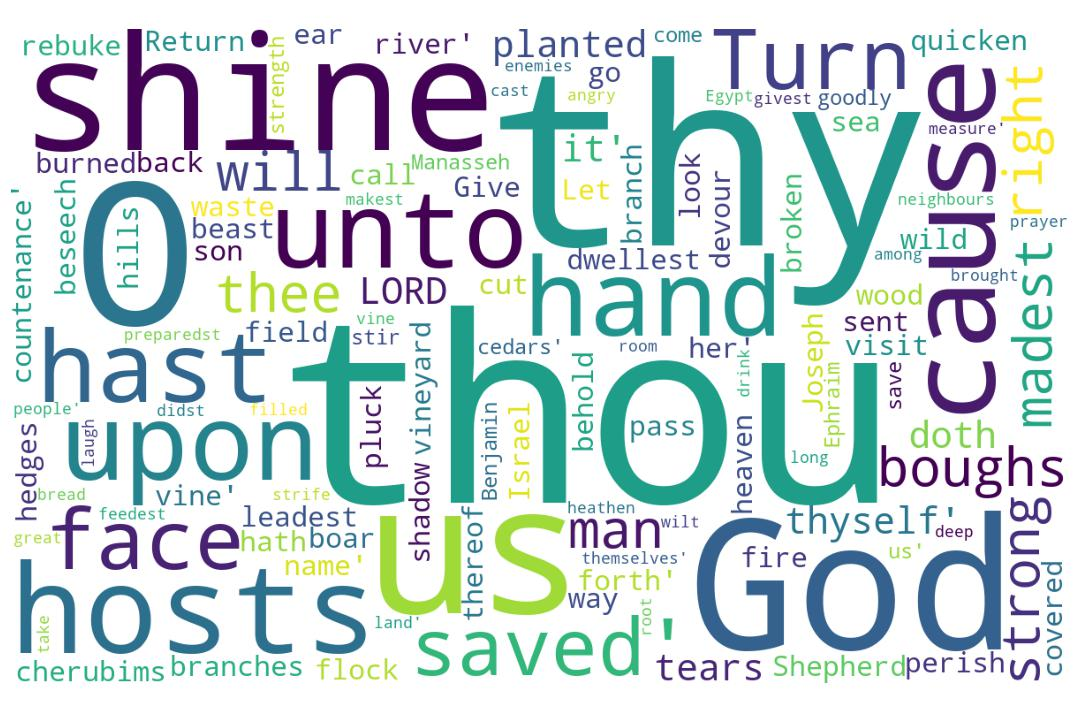
\includegraphics[width=\linewidth]{19OT-Psalms/Psalm80-WordCloud.jpg}
  \caption{Psalm 80 Word Cloud}
  \label{fig:Psalm 80 word Cloud}
\end{figure}

\marginpar{\scriptsize \centering \fcolorbox{bone}{lime}{\textbf{TURN US, LORD}}\\ (Psalm 80:1-19) \begin{compactenum}[I.][8]
     \item The \textbf{Envisioned Power} \index[scripture]{Psalms!Psa 080:01}(Psa 80:1)
     \item The \textbf{Vile and Vilified People} \index[scripture]{Psalms!Psa 080:06}(Psa 80:6)
     \item A \textbf{Vine Planted} \index[scripture]{Psalms!Psa 080:08}(Psa 80:8)
     \item A \textbf{Visit Proposed} \index[scripture]{Psalms!Psa 080:14}(Psa 80:14)
     \item A \textbf{Vineyard Pulled Down} \index[scripture]{Psalms!Psa 080:16}(Psa 80:16)
     \item The \textbf{Victor Empowered} \index[scripture]{Psalms!Psa 080:17}(Psa 80:17)
     \item The \textbf{Revitalized People} \index[scripture]{Psalms!Psa 080:19}(Psa 80:19)
\end{compactenum}}


\footnote{\textcolor[rgb]{0.00,0.25,0.00}{\hyperlink{TOC}{Return to end of Table of Contents.}}}
\footnote{\href{https://audiobible.com/bible/psalms_80.html}{\textcolor[cmyk]{0.99998,1,0,0}{Psalm 80 Audio}}}\textcolor[cmyk]{0.99998,1,0,0}{To the chief Musician upon Shoshannim-Eduth, A Psalm of Asaph.}\\
\\
\textcolor[cmyk]{0.99998,1,0,0}{Give ear, O Shepherd of Israel, thou that leadest Joseph like a flock; thou that dwellest \emph{between} the cherubims, shine forth.}
[2] \textcolor[cmyk]{0.99998,1,0,0}{Before Ephraim and Benjamin and Manasseh stir up thy strength, and come \emph{and} save us.}
[3] \textcolor[cmyk]{0.99998,1,0,0}{\fcolorbox{black}{red}{Turn us} again, O God, and cause thy face to shine; and we shall be saved.}
[4] \textcolor[cmyk]{0.99998,1,0,0}{O LORD God of hosts, how long wilt thou be angry against the prayer of thy people?}
[5] \textcolor[cmyk]{0.99998,1,0,0}{Thou feedest them with the bread of tears; and givest them tears to drink in great measure.}\footnote{\textbf{Deuteronomy 16:3} - Thou shalt eat no leavened bread with it; seven days shalt thou eat unleavened bread therewith, even the bread of affliction; for thou camest forth out of the land of Egypt in haste: that thou mayest remember the day when thou camest forth out of the land of Egypt all the days of thy life.}
[6] \textcolor[cmyk]{0.99998,1,0,0}{Thou makest us a strife unto our neighbours: and our enemies laugh among themselves.}
[7] \textcolor[cmyk]{0.99998,1,0,0}{\fcolorbox{black}{red}{Turn us} again, O God of hosts, and cause thy face to shine; and we shall be saved.}
[8] \textcolor[cmyk]{0.99998,1,0,0}{Thou hast brought a vine out of Egypt: thou hast cast out the heathen, and planted it.}
[9] \textcolor[cmyk]{0.99998,1,0,0}{Thou preparedst \emph{room} before it, and didst cause it to take deep root, and it filled the land.}
[10] \textcolor[cmyk]{0.99998,1,0,0}{The hills were covered with the shadow of it, and the boughs thereof \emph{were} \emph{like} the goodly cedars.}
[11] \textcolor[cmyk]{0.99998,1,0,0}{She sent out her boughs unto the sea, and her branches unto the river.}
[12] \textcolor[cmyk]{0.99998,1,0,0}{Why hast thou \emph{then} broken down her hedges, so that all they which pass by the way do pluck her?}
[13] \textcolor[cmyk]{0.99998,1,0,0}{The boar out of the wood doth waste it, and the wild beast of the field doth devour it.}
[14] \textcolor[cmyk]{0.99998,1,0,0}{Return, we beseech thee, O God of hosts: look down from heaven, and behold, and visit this vine;}
[15] \textcolor[cmyk]{0.99998,1,0,0}{And the vineyard which thy right hand hath planted, and the branch \emph{that} thou madest strong for thyself.}
[16] \textcolor[cmyk]{0.99998,1,0,0}{\emph{It} \emph{is} burned with fire, \emph{it} \emph{is} cut down: they perish at the rebuke of thy countenance.}
[17] \textcolor[cmyk]{0.99998,1,0,0}{Let thy hand be upon the man of thy right hand, upon the son of man \emph{whom} thou madest strong for thyself.}
[18] \textcolor[cmyk]{0.99998,1,0,0}{So will not we go back from thee: quicken us, and we will call upon thy name.}
[19] \textcolor[cmyk]{0.99998,1,0,0}{\fcolorbox{black}{red}{Turn us} again, O LORD God of hosts, cause thy face to shine; and we shall be saved.}\footnote{\textbf{Ezekiel 18:31} - Cast away from you all your transgressions, whereby ye have transgressed; and make you a new heart and a new spirit: for why will ye die, O house of Israel?}\footnote{\textbf{Ezekiel 36:26-28} - A new heart also will I give you, and a new spirit will I put within you: and I will take away the stony heart out of your flesh, and I will give you an heart of flesh. [27] And I will put my spirit within you, and cause you to walk in my statutes, and ye shall keep my judgments, and do them. [28] And ye shall dwell in the land that I gave to your fathers; and ye shall be my people, and I will be your God.}
\index[NWIV]{21!Psa!Psa 80:1}\index[AWIP]{Give!Psa!Psa 80:1}\index[AWIP]{ear!Psa!Psa 80:1}\index[AWIP]{O!Psa!Psa 80:1}\index[AWIP]{Shepherd!Psa!Psa 80:1}\index[AWIP]{of!Psa!Psa 80:1}\index[AWIP]{Israel!Psa!Psa 80:1}\index[AWIP]{thou!Psa!Psa 80:1}\index[AWIP]{thou!Psa!Psa 80:1 (2)}\index[AWIP]{that!Psa!Psa 80:1}\index[AWIP]{that!Psa!Psa 80:1 (2)}\index[AWIP]{leadest!Psa!Psa 80:1}\index[AWIP]{Joseph!Psa!Psa 80:1}\index[AWIP]{like!Psa!Psa 80:1}\index[AWIP]{a!Psa!Psa 80:1}\index[AWIP]{flock!Psa!Psa 80:1}\index[AWIP]{dwellest!Psa!Psa 80:1}\index[AWIP]{\emph{between}!Psa!Psa 80:1}\index[AWIP]{the!Psa!Psa 80:1}\index[AWIP]{cherubims!Psa!Psa 80:1}\index[AWIP]{shine!Psa!Psa 80:1}\index[AWIP]{forth!Psa!Psa 80:1}\index[AWIP]{\emph{between}!Psa!Psa 80:1}

\index[NWIV]{15!Psa!Psa 80:2}\index[AWIP]{Before!Psa!Psa 80:2}\index[AWIP]{Ephraim!Psa!Psa 80:2}\index[AWIP]{and!Psa!Psa 80:2}\index[AWIP]{and!Psa!Psa 80:2 (2)}\index[AWIP]{and!Psa!Psa 80:2 (3)}\index[AWIP]{Benjamin!Psa!Psa 80:2}\index[AWIP]{Manasseh!Psa!Psa 80:2}\index[AWIP]{stir!Psa!Psa 80:2}\index[AWIP]{up!Psa!Psa 80:2}\index[AWIP]{thy!Psa!Psa 80:2}\index[AWIP]{strength!Psa!Psa 80:2}\index[AWIP]{come!Psa!Psa 80:2}\index[AWIP]{\emph{and}!Psa!Psa 80:2}\index[AWIP]{save!Psa!Psa 80:2}\index[AWIP]{us!Psa!Psa 80:2}\index[AWIP]{\emph{and}!Psa!Psa 80:2}

\index[NWIV]{16!Psa!Psa 80:3}\index[AWIP]{Turn!Psa!Psa 80:3}\index[AWIP]{us!Psa!Psa 80:3}\index[AWIP]{again!Psa!Psa 80:3}\index[AWIP]{O!Psa!Psa 80:3}\index[AWIP]{God!Psa!Psa 80:3}\index[AWIP]{and!Psa!Psa 80:3}\index[AWIP]{and!Psa!Psa 80:3 (2)}\index[AWIP]{cause!Psa!Psa 80:3}\index[AWIP]{thy!Psa!Psa 80:3}\index[AWIP]{face!Psa!Psa 80:3}\index[AWIP]{to!Psa!Psa 80:3}\index[AWIP]{shine!Psa!Psa 80:3}\index[AWIP]{we!Psa!Psa 80:3}\index[AWIP]{shall!Psa!Psa 80:3}\index[AWIP]{be!Psa!Psa 80:3}\index[AWIP]{saved!Psa!Psa 80:3}

\index[NWIV]{17!Psa!Psa 80:4}\index[AWIP]{O!Psa!Psa 80:4}\index[AWIP]{LORD!Psa!Psa 80:4}\index[AWIP]{God!Psa!Psa 80:4}\index[AWIP]{of!Psa!Psa 80:4}\index[AWIP]{of!Psa!Psa 80:4 (2)}\index[AWIP]{hosts!Psa!Psa 80:4}\index[AWIP]{how!Psa!Psa 80:4}\index[AWIP]{long!Psa!Psa 80:4}\index[AWIP]{wilt!Psa!Psa 80:4}\index[AWIP]{thou!Psa!Psa 80:4}\index[AWIP]{be!Psa!Psa 80:4}\index[AWIP]{angry!Psa!Psa 80:4}\index[AWIP]{against!Psa!Psa 80:4}\index[AWIP]{the!Psa!Psa 80:4}\index[AWIP]{prayer!Psa!Psa 80:4}\index[AWIP]{thy!Psa!Psa 80:4}\index[AWIP]{people?!Psa!Psa 80:4}

\index[NWIV]{17!Psa!Psa 80:5}\index[AWIP]{Thou!Psa!Psa 80:5}\index[AWIP]{feedest!Psa!Psa 80:5}\index[AWIP]{them!Psa!Psa 80:5}\index[AWIP]{them!Psa!Psa 80:5 (2)}\index[AWIP]{with!Psa!Psa 80:5}\index[AWIP]{the!Psa!Psa 80:5}\index[AWIP]{bread!Psa!Psa 80:5}\index[AWIP]{of!Psa!Psa 80:5}\index[AWIP]{tears!Psa!Psa 80:5}\index[AWIP]{tears!Psa!Psa 80:5 (2)}\index[AWIP]{and!Psa!Psa 80:5}\index[AWIP]{givest!Psa!Psa 80:5}\index[AWIP]{to!Psa!Psa 80:5}\index[AWIP]{drink!Psa!Psa 80:5}\index[AWIP]{in!Psa!Psa 80:5}\index[AWIP]{great!Psa!Psa 80:5}\index[AWIP]{measure!Psa!Psa 80:5}

\index[NWIV]{14!Psa!Psa 80:6}\index[AWIP]{Thou!Psa!Psa 80:6}\index[AWIP]{makest!Psa!Psa 80:6}\index[AWIP]{us!Psa!Psa 80:6}\index[AWIP]{a!Psa!Psa 80:6}\index[AWIP]{strife!Psa!Psa 80:6}\index[AWIP]{unto!Psa!Psa 80:6}\index[AWIP]{our!Psa!Psa 80:6}\index[AWIP]{our!Psa!Psa 80:6 (2)}\index[AWIP]{neighbours!Psa!Psa 80:6}\index[AWIP]{and!Psa!Psa 80:6}\index[AWIP]{enemies!Psa!Psa 80:6}\index[AWIP]{laugh!Psa!Psa 80:6}\index[AWIP]{among!Psa!Psa 80:6}\index[AWIP]{themselves!Psa!Psa 80:6}

\index[NWIV]{18!Psa!Psa 80:7}\index[AWIP]{Turn!Psa!Psa 80:7}\index[AWIP]{us!Psa!Psa 80:7}\index[AWIP]{again!Psa!Psa 80:7}\index[AWIP]{O!Psa!Psa 80:7}\index[AWIP]{God!Psa!Psa 80:7}\index[AWIP]{of!Psa!Psa 80:7}\index[AWIP]{hosts!Psa!Psa 80:7}\index[AWIP]{and!Psa!Psa 80:7}\index[AWIP]{and!Psa!Psa 80:7 (2)}\index[AWIP]{cause!Psa!Psa 80:7}\index[AWIP]{thy!Psa!Psa 80:7}\index[AWIP]{face!Psa!Psa 80:7}\index[AWIP]{to!Psa!Psa 80:7}\index[AWIP]{shine!Psa!Psa 80:7}\index[AWIP]{we!Psa!Psa 80:7}\index[AWIP]{shall!Psa!Psa 80:7}\index[AWIP]{be!Psa!Psa 80:7}\index[AWIP]{saved!Psa!Psa 80:7}

\index[NWIV]{17!Psa!Psa 80:8}\index[AWIP]{Thou!Psa!Psa 80:8}\index[AWIP]{hast!Psa!Psa 80:8}\index[AWIP]{hast!Psa!Psa 80:8 (2)}\index[AWIP]{brought!Psa!Psa 80:8}\index[AWIP]{a!Psa!Psa 80:8}\index[AWIP]{vine!Psa!Psa 80:8}\index[AWIP]{out!Psa!Psa 80:8}\index[AWIP]{out!Psa!Psa 80:8 (2)}\index[AWIP]{of!Psa!Psa 80:8}\index[AWIP]{Egypt!Psa!Psa 80:8}\index[AWIP]{thou!Psa!Psa 80:8}\index[AWIP]{cast!Psa!Psa 80:8}\index[AWIP]{the!Psa!Psa 80:8}\index[AWIP]{heathen!Psa!Psa 80:8}\index[AWIP]{and!Psa!Psa 80:8}\index[AWIP]{planted!Psa!Psa 80:8}\index[AWIP]{it!Psa!Psa 80:8}

\index[NWIV]{18!Psa!Psa 80:9}\index[AWIP]{Thou!Psa!Psa 80:9}\index[AWIP]{preparedst!Psa!Psa 80:9}\index[AWIP]{\emph{room}!Psa!Psa 80:9}\index[AWIP]{before!Psa!Psa 80:9}\index[AWIP]{it!Psa!Psa 80:9}\index[AWIP]{it!Psa!Psa 80:9 (2)}\index[AWIP]{it!Psa!Psa 80:9 (3)}\index[AWIP]{and!Psa!Psa 80:9}\index[AWIP]{and!Psa!Psa 80:9 (2)}\index[AWIP]{didst!Psa!Psa 80:9}\index[AWIP]{cause!Psa!Psa 80:9}\index[AWIP]{to!Psa!Psa 80:9}\index[AWIP]{take!Psa!Psa 80:9}\index[AWIP]{deep!Psa!Psa 80:9}\index[AWIP]{root!Psa!Psa 80:9}\index[AWIP]{filled!Psa!Psa 80:9}\index[AWIP]{the!Psa!Psa 80:9}\index[AWIP]{land!Psa!Psa 80:9}\index[AWIP]{\emph{room}!Psa!Psa 80:9}

\index[NWIV]{18!Psa!Psa 80:10}\index[AWIP]{The!Psa!Psa 80:10}\index[AWIP]{hills!Psa!Psa 80:10}\index[AWIP]{were!Psa!Psa 80:10}\index[AWIP]{covered!Psa!Psa 80:10}\index[AWIP]{with!Psa!Psa 80:10}\index[AWIP]{the!Psa!Psa 80:10}\index[AWIP]{the!Psa!Psa 80:10 (2)}\index[AWIP]{the!Psa!Psa 80:10 (3)}\index[AWIP]{shadow!Psa!Psa 80:10}\index[AWIP]{of!Psa!Psa 80:10}\index[AWIP]{it!Psa!Psa 80:10}\index[AWIP]{and!Psa!Psa 80:10}\index[AWIP]{boughs!Psa!Psa 80:10}\index[AWIP]{thereof!Psa!Psa 80:10}\index[AWIP]{\emph{were}!Psa!Psa 80:10}\index[AWIP]{\emph{like}!Psa!Psa 80:10}\index[AWIP]{goodly!Psa!Psa 80:10}\index[AWIP]{cedars!Psa!Psa 80:10}\index[AWIP]{\emph{were}!Psa!Psa 80:10}\index[AWIP]{\emph{like}!Psa!Psa 80:10}

\index[NWIV]{14!Psa!Psa 80:11}\index[AWIP]{She!Psa!Psa 80:11}\index[AWIP]{sent!Psa!Psa 80:11}\index[AWIP]{out!Psa!Psa 80:11}\index[AWIP]{her!Psa!Psa 80:11}\index[AWIP]{her!Psa!Psa 80:11 (2)}\index[AWIP]{boughs!Psa!Psa 80:11}\index[AWIP]{unto!Psa!Psa 80:11}\index[AWIP]{unto!Psa!Psa 80:11 (2)}\index[AWIP]{the!Psa!Psa 80:11}\index[AWIP]{the!Psa!Psa 80:11 (2)}\index[AWIP]{sea!Psa!Psa 80:11}\index[AWIP]{and!Psa!Psa 80:11}\index[AWIP]{branches!Psa!Psa 80:11}\index[AWIP]{river!Psa!Psa 80:11}

\index[NWIV]{20!Psa!Psa 80:12}\index[AWIP]{Why!Psa!Psa 80:12}\index[AWIP]{hast!Psa!Psa 80:12}\index[AWIP]{thou!Psa!Psa 80:12}\index[AWIP]{\emph{then}!Psa!Psa 80:12}\index[AWIP]{broken!Psa!Psa 80:12}\index[AWIP]{down!Psa!Psa 80:12}\index[AWIP]{her!Psa!Psa 80:12}\index[AWIP]{hedges!Psa!Psa 80:12}\index[AWIP]{so!Psa!Psa 80:12}\index[AWIP]{that!Psa!Psa 80:12}\index[AWIP]{all!Psa!Psa 80:12}\index[AWIP]{they!Psa!Psa 80:12}\index[AWIP]{which!Psa!Psa 80:12}\index[AWIP]{pass!Psa!Psa 80:12}\index[AWIP]{by!Psa!Psa 80:12}\index[AWIP]{the!Psa!Psa 80:12}\index[AWIP]{way!Psa!Psa 80:12}\index[AWIP]{do!Psa!Psa 80:12}\index[AWIP]{pluck!Psa!Psa 80:12}\index[AWIP]{her?!Psa!Psa 80:12}\index[AWIP]{\emph{then}!Psa!Psa 80:12}

\index[NWIV]{19!Psa!Psa 80:13}\index[AWIP]{The!Psa!Psa 80:13}\index[AWIP]{boar!Psa!Psa 80:13}\index[AWIP]{out!Psa!Psa 80:13}\index[AWIP]{of!Psa!Psa 80:13}\index[AWIP]{of!Psa!Psa 80:13 (2)}\index[AWIP]{the!Psa!Psa 80:13}\index[AWIP]{the!Psa!Psa 80:13 (2)}\index[AWIP]{the!Psa!Psa 80:13 (3)}\index[AWIP]{wood!Psa!Psa 80:13}\index[AWIP]{doth!Psa!Psa 80:13}\index[AWIP]{doth!Psa!Psa 80:13 (2)}\index[AWIP]{waste!Psa!Psa 80:13}\index[AWIP]{it!Psa!Psa 80:13}\index[AWIP]{it!Psa!Psa 80:13 (2)}\index[AWIP]{and!Psa!Psa 80:13}\index[AWIP]{wild!Psa!Psa 80:13}\index[AWIP]{beast!Psa!Psa 80:13}\index[AWIP]{field!Psa!Psa 80:13}\index[AWIP]{devour!Psa!Psa 80:13}

\index[NWIV]{18!Psa!Psa 80:14}\index[AWIP]{Return!Psa!Psa 80:14}\index[AWIP]{we!Psa!Psa 80:14}\index[AWIP]{beseech!Psa!Psa 80:14}\index[AWIP]{thee!Psa!Psa 80:14}\index[AWIP]{O!Psa!Psa 80:14}\index[AWIP]{God!Psa!Psa 80:14}\index[AWIP]{of!Psa!Psa 80:14}\index[AWIP]{hosts!Psa!Psa 80:14}\index[AWIP]{look!Psa!Psa 80:14}\index[AWIP]{down!Psa!Psa 80:14}\index[AWIP]{from!Psa!Psa 80:14}\index[AWIP]{heaven!Psa!Psa 80:14}\index[AWIP]{and!Psa!Psa 80:14}\index[AWIP]{and!Psa!Psa 80:14 (2)}\index[AWIP]{behold!Psa!Psa 80:14}\index[AWIP]{visit!Psa!Psa 80:14}\index[AWIP]{this!Psa!Psa 80:14}\index[AWIP]{vine!Psa!Psa 80:14}

\index[NWIV]{18!Psa!Psa 80:15}\index[AWIP]{And!Psa!Psa 80:15}\index[AWIP]{the!Psa!Psa 80:15}\index[AWIP]{the!Psa!Psa 80:15 (2)}\index[AWIP]{vineyard!Psa!Psa 80:15}\index[AWIP]{which!Psa!Psa 80:15}\index[AWIP]{thy!Psa!Psa 80:15}\index[AWIP]{right!Psa!Psa 80:15}\index[AWIP]{hand!Psa!Psa 80:15}\index[AWIP]{hath!Psa!Psa 80:15}\index[AWIP]{planted!Psa!Psa 80:15}\index[AWIP]{and!Psa!Psa 80:15}\index[AWIP]{branch!Psa!Psa 80:15}\index[AWIP]{\emph{that}!Psa!Psa 80:15}\index[AWIP]{thou!Psa!Psa 80:15}\index[AWIP]{madest!Psa!Psa 80:15}\index[AWIP]{strong!Psa!Psa 80:15}\index[AWIP]{for!Psa!Psa 80:15}\index[AWIP]{thyself!Psa!Psa 80:15}\index[AWIP]{\emph{that}!Psa!Psa 80:15}

\index[NWIV]{17!Psa!Psa 80:16}\index[AWIP]{\emph{It}!Psa!Psa 80:16}\index[AWIP]{\emph{is}!Psa!Psa 80:16}\index[AWIP]{\emph{is}!Psa!Psa 80:16 (2)}\index[AWIP]{burned!Psa!Psa 80:16}\index[AWIP]{with!Psa!Psa 80:16}\index[AWIP]{fire!Psa!Psa 80:16}\index[AWIP]{\emph{it}!Psa!Psa 80:16}\index[AWIP]{cut!Psa!Psa 80:16}\index[AWIP]{down!Psa!Psa 80:16}\index[AWIP]{they!Psa!Psa 80:16}\index[AWIP]{perish!Psa!Psa 80:16}\index[AWIP]{at!Psa!Psa 80:16}\index[AWIP]{the!Psa!Psa 80:16}\index[AWIP]{rebuke!Psa!Psa 80:16}\index[AWIP]{of!Psa!Psa 80:16}\index[AWIP]{thy!Psa!Psa 80:16}\index[AWIP]{countenance!Psa!Psa 80:16}\index[AWIP]{\emph{It}!Psa!Psa 80:16}\index[AWIP]{\emph{is}!Psa!Psa 80:16}\index[AWIP]{\emph{is}!Psa!Psa 80:16 (2)}\index[AWIP]{\emph{it}!Psa!Psa 80:16}

\index[NWIV]{22!Psa!Psa 80:17}\index[AWIP]{Let!Psa!Psa 80:17}\index[AWIP]{thy!Psa!Psa 80:17}\index[AWIP]{thy!Psa!Psa 80:17 (2)}\index[AWIP]{hand!Psa!Psa 80:17}\index[AWIP]{hand!Psa!Psa 80:17 (2)}\index[AWIP]{be!Psa!Psa 80:17}\index[AWIP]{upon!Psa!Psa 80:17}\index[AWIP]{upon!Psa!Psa 80:17 (2)}\index[AWIP]{the!Psa!Psa 80:17}\index[AWIP]{the!Psa!Psa 80:17 (2)}\index[AWIP]{man!Psa!Psa 80:17}\index[AWIP]{man!Psa!Psa 80:17 (2)}\index[AWIP]{of!Psa!Psa 80:17}\index[AWIP]{of!Psa!Psa 80:17 (2)}\index[AWIP]{right!Psa!Psa 80:17}\index[AWIP]{son!Psa!Psa 80:17}\index[AWIP]{\emph{whom}!Psa!Psa 80:17}\index[AWIP]{thou!Psa!Psa 80:17}\index[AWIP]{madest!Psa!Psa 80:17}\index[AWIP]{strong!Psa!Psa 80:17}\index[AWIP]{for!Psa!Psa 80:17}\index[AWIP]{thyself!Psa!Psa 80:17}\index[AWIP]{\emph{whom}!Psa!Psa 80:17}

\index[NWIV]{17!Psa!Psa 80:18}\index[AWIP]{So!Psa!Psa 80:18}\index[AWIP]{will!Psa!Psa 80:18}\index[AWIP]{will!Psa!Psa 80:18 (2)}\index[AWIP]{not!Psa!Psa 80:18}\index[AWIP]{we!Psa!Psa 80:18}\index[AWIP]{we!Psa!Psa 80:18 (2)}\index[AWIP]{go!Psa!Psa 80:18}\index[AWIP]{back!Psa!Psa 80:18}\index[AWIP]{from!Psa!Psa 80:18}\index[AWIP]{thee!Psa!Psa 80:18}\index[AWIP]{quicken!Psa!Psa 80:18}\index[AWIP]{us!Psa!Psa 80:18}\index[AWIP]{and!Psa!Psa 80:18}\index[AWIP]{call!Psa!Psa 80:18}\index[AWIP]{upon!Psa!Psa 80:18}\index[AWIP]{thy!Psa!Psa 80:18}\index[AWIP]{name!Psa!Psa 80:18}

\index[NWIV]{18!Psa!Psa 80:19}\index[AWIP]{Turn!Psa!Psa 80:19}\index[AWIP]{us!Psa!Psa 80:19}\index[AWIP]{again!Psa!Psa 80:19}\index[AWIP]{O!Psa!Psa 80:19}\index[AWIP]{LORD!Psa!Psa 80:19}\index[AWIP]{God!Psa!Psa 80:19}\index[AWIP]{of!Psa!Psa 80:19}\index[AWIP]{hosts!Psa!Psa 80:19}\index[AWIP]{cause!Psa!Psa 80:19}\index[AWIP]{thy!Psa!Psa 80:19}\index[AWIP]{face!Psa!Psa 80:19}\index[AWIP]{to!Psa!Psa 80:19}\index[AWIP]{shine!Psa!Psa 80:19}\index[AWIP]{and!Psa!Psa 80:19}\index[AWIP]{we!Psa!Psa 80:19}\index[AWIP]{shall!Psa!Psa 80:19}\index[AWIP]{be!Psa!Psa 80:19}\index[AWIP]{saved!Psa!Psa 80:19}


\section{Psalm 80 Outlines}

\subsection{My Outlines}

\subsubsection{Turn Us, Lord!}

\index[speaker]{Keith Anthony!Psalm 080 (Turn Us, Lord)}
\index[series]{Psalms (Keith Anthony)!Psalm 080 (Turn Us, Lord)}
\index[date]{2015/06/04!Psalm 080 (Turn Us, Lord) (Keith Anthony)}

\begin{compactenum}[I.]
     \item The \textbf{Envisioned Power} \index[scripture]{Psalms!Psa 080:01}(Psa 80:1)
     \item The \textbf{Vile and Vilified People} \index[scripture]{Psalms!Psa 080:06}(Psa 80:6)
     \item A \textbf{Vine Planted} \index[scripture]{Psalms!Psa 080:08}(Psa 80:8)
     \item A \textbf{Visit Proposed} \index[scripture]{Psalms!Psa 080:14}(Psa 80:14)
     \item A \textbf{Vineyard Pulled Down} \index[scripture]{Psalms!Psa 080:16}(Psa 80:16)
     \item The \textbf{Victor Empowered} \index[scripture]{Psalms!Psa 080:17}(Psa 80:17)
     \item The \textbf{Revitalized People} \index[scripture]{Psalms!Psa 080:19}(Psa 80:19)
\end{compactenum}


\subsection{Outlines from Others}


\section{Psalm 80 Comments}

\subsection{Numeric  Nuggets}
Verses 2, and 6 have 13 unique words.  The phrase ``cause thy face to shine and we shall be saved'' is found 3 times in verses 3, 7, and 19, with the verses beginning with ``Turn us again.'' The three instances may be historically (and prophetically) indicative of three great deliverances of the people of Israel.
\subsection{Psalm 80 Repeated Phrases}


%%%%%%%%%%
%%%%%%%%%%
\normalsize
 
\begin{center}
\begin{longtable}{|p{3.0in}|p{0.5in}|}
\caption[Psalm 80 Repeated Phrases]{Psalm 80 Repeated Phrases}\label{table:Repeated Phrases Psalm 80} \\
\hline \multicolumn{1}{|c|}{\textbf{Phrase}} & \multicolumn{1}{c|}{\textbf{Frequency}} \\ \hline 
\endfirsthead
 
\multicolumn{2}{c}
{{\bfseries \tablename\ \thetable{} -- continued from previous page}} \\  
\hline \multicolumn{1}{|c|}{\textbf{Phrase}} & \multicolumn{1}{c|}{\textbf{Frequency}} \\ \hline 
\endhead
 
\hline \multicolumn{2}{c}{{ }} \\ \hline
\endfoot 
and we & 4\\ \hline 
God of & 4\\ \hline 
God of hosts & 4\\ \hline 
of hosts & 4\\ \hline 
Turn us & 3\\ \hline 
Turn us again & 3\\ \hline 
Turn us again O & 3\\ \hline 
us again & 3\\ \hline 
us again O & 3\\ \hline 
again O & 3\\ \hline 
O God & 3\\ \hline 
cause thy & 3\\ \hline 
cause thy face & 3\\ \hline 
cause thy face to & 3\\ \hline 
cause thy face to shine & 3\\ \hline 
cause thy face to shine and & 3\\ \hline 
cause thy face to shine and we & 3\\ \hline 
cause thy face to shine and we shall & 3\\ \hline 
cause thy face to shine and we shall be & 3\\ \hline 
cause thy face to shine and we shall be saved & 3\\ \hline 
thy face & 3\\ \hline 
thy face to & 3\\ \hline 
thy face to shine & 3\\ \hline 
thy face to shine and & 3\\ \hline 
thy face to shine and we & 3\\ \hline 
thy face to shine and we shall & 3\\ \hline 
thy face to shine and we shall be & 3\\ \hline 
thy face to shine and we shall be saved & 3\\ \hline 
face to & 3\\ \hline 
face to shine & 3\\ \hline 
face to shine and & 3\\ \hline 
face to shine and we & 3\\ \hline 
face to shine and we shall & 3\\ \hline 
face to shine and we shall be & 3\\ \hline 
face to shine and we shall be saved & 3\\ \hline 
to shine & 3\\ \hline 
to shine and & 3\\ \hline 
to shine and we & 3\\ \hline 
to shine and we shall & 3\\ \hline 
to shine and we shall be & 3\\ \hline 
to shine and we shall be saved & 3\\ \hline 
shine and & 3\\ \hline 
shine and we & 3\\ \hline 
shine and we shall & 3\\ \hline 
shine and we shall be & 3\\ \hline 
shine and we shall be saved & 3\\ \hline 
and we shall & 3\\ \hline 
and we shall be & 3\\ \hline 
and we shall be saved & 3\\ \hline 
we shall & 3\\ \hline 
we shall be & 3\\ \hline 
we shall be saved & 3\\ \hline 
shall be & 3\\ \hline 
shall be saved & 3\\ \hline 
be saved & 3\\ \hline 
of thy & 3\\ \hline 
it and & 3\\ \hline 
and the & 3\\ \hline 
\end{longtable}
\end{center}



%%%%%%%%%%
%%%%%%%%%%



\section{Psalm 80 Statistics}

%%%%%%%%%%%%%%%%%%%%%%%%%%%
%%%%% Word Statistics
%%%%%%%%%%%%%%%%%%%%%%%%%%


\normalsize



\subsection{Chapter Word Statistics}


%%%%%%%%%%
%%%%%%%%%%
 
\begin{center}
\begin{longtable}{l|c|c|c|c}
\caption[Stats for Psalm 80]{Stats for Psalm 80} \label{table:Stats for Psalm 80} \\ 
\hline \multicolumn{1}{|c|}{\textbf{Verse(s)}} & \multicolumn{1}{|c|}{\textbf{Count}} & \multicolumn{1}{|c|}{\textbf{Unique}} & \multicolumn{1}{|c|}{\textbf{Italics}} & \multicolumn{1}{|c|}{\textbf{Uniq Italic}}  \\ \hline 
\endfirsthead
 
\multicolumn{5}{c}
{{\bfseries \tablename\ \thetable{} -- continued from previous page}} \\  
\hline \multicolumn{1}{|c|}{\textbf{Verse(s)}} & \multicolumn{1}{|c|}{\textbf{Count}} & \multicolumn{1}{|c|}{\textbf{Unique}} & \multicolumn{1}{|c|}{\textbf{Italics}} & \multicolumn{1}{|c|}{\textbf{Uniq Italic}}  \\ \hline 
\endhead
 
\hline \multicolumn{5}{|r|}{{Continued if needed}} \\ \hline
\endfoot 
1 & 21 & 19 & 1 & 1\\ \hline
2 & 15 & 13 & 1 & 1\\ \hline
3 & 16 & 15 & 0 & 0\\ \hline
4 & 17 & 16 & 0 & 0\\ \hline
5 & 17 & 15 & 0 & 0\\ \hline
6 & 14 & 13 & 0 & 0\\ \hline
7 & 18 & 17 & 0 & 0\\ \hline
8 & 17 & 15 & 0 & 0\\ \hline
9 & 18 & 15 & 1 & 1\\ \hline
10 & 18 & 16 & 2 & 2\\ \hline
11 & 14 & 11 & 0 & 0\\ \hline
12 & 20 & 19 & 1 & 1\\ \hline
13 & 19 & 14 & 0 & 0\\ \hline
14 & 18 & 17 & 0 & 0\\ \hline
15 & 18 & 17 & 1 & 1\\ \hline
16 & 17 & 16 & 4 & 3\\ \hline
17 & 22 & 16 & 1 & 1\\ \hline
18 & 17 & 15 & 0 & 0\\ \hline
19 & 18 & 18 & 0 & 0\\ \hline
\hline \hline
Total & 334 & 171 & 12 & 11



\end{longtable}
\end{center}

%%%%%%%%%%
%%%%%%%%%%
 
\subsection{Words by Frequency}

\begin{center}
\begin{longtable}{l|r}
\caption[Word Frequencies in Psalm 80]{Word Frequencies in Psalm 80} \label{table:WordsIn-Psalm-80} \\ 
\hline \multicolumn{1}{|c|}{\textbf{Word}} & \multicolumn{1}{c|}{\textbf{Frequency}} \\ \hline 
\endfirsthead
 
\multicolumn{2}{c}
{{\bfseries \tablename\ \thetable{} -- continued from previous page}} \\ 
\hline \multicolumn{1}{|c|}{\textbf{Word}} & \multicolumn{1}{c|}{\textbf{Frequency}} \\ \hline 
\endhead
 
\hline \multicolumn{2}{|r|}{{Continued if needed}} \\ \hline
\endfoot
 
\hline \hline
\endlastfoot
and & 20 \\ \hline
the & 19 \\ \hline
of & 14 \\ \hline
thy & 10 \\ \hline
thou & 7 \\ \hline
it & 7 \\ \hline
O & 6 \\ \hline
us & 6 \\ \hline
we & 6 \\ \hline
God & 5 \\ \hline
to & 5 \\ \hline
be & 5 \\ \hline
shine & 4 \\ \hline
cause & 4 \\ \hline
hosts & 4 \\ \hline
Thou & 4 \\ \hline
out & 4 \\ \hline
her & 4 \\ \hline
that & 3 \\ \hline
a & 3 \\ \hline
Turn & 3 \\ \hline
again & 3 \\ \hline
face & 3 \\ \hline
shall & 3 \\ \hline
saved & 3 \\ \hline
with & 3 \\ \hline
unto & 3 \\ \hline
hast & 3 \\ \hline
down & 3 \\ \hline
hand & 3 \\ \hline
upon & 3 \\ \hline
LORD & 2 \\ \hline
them & 2 \\ \hline
tears & 2 \\ \hline
our & 2 \\ \hline
vine & 2 \\ \hline
planted & 2 \\ \hline
The & 2 \\ \hline
boughs & 2 \\ \hline
they & 2 \\ \hline
which & 2 \\ \hline
doth & 2 \\ \hline
thee & 2 \\ \hline
from & 2 \\ \hline
right & 2 \\ \hline
madest & 2 \\ \hline
strong & 2 \\ \hline
for & 2 \\ \hline
thyself & 2 \\ \hline
\emph{is} & 2 \\ \hline
man & 2 \\ \hline
will & 2 \\ \hline
Give & 1 \\ \hline
ear & 1 \\ \hline
Shepherd & 1 \\ \hline
Israel & 1 \\ \hline
leadest & 1 \\ \hline
Joseph & 1 \\ \hline
like & 1 \\ \hline
flock & 1 \\ \hline
dwellest & 1 \\ \hline
\emph{between} & 1 \\ \hline
cherubims & 1 \\ \hline
forth & 1 \\ \hline
Before & 1 \\ \hline
Ephraim & 1 \\ \hline
Benjamin & 1 \\ \hline
Manasseh & 1 \\ \hline
stir & 1 \\ \hline
up & 1 \\ \hline
strength & 1 \\ \hline
come & 1 \\ \hline
\emph{and} & 1 \\ \hline
save & 1 \\ \hline
how & 1 \\ \hline
long & 1 \\ \hline
wilt & 1 \\ \hline
angry & 1 \\ \hline
against & 1 \\ \hline
prayer & 1 \\ \hline
people & 1 \\ \hline
feedest & 1 \\ \hline
bread & 1 \\ \hline
givest & 1 \\ \hline
drink & 1 \\ \hline
in & 1 \\ \hline
great & 1 \\ \hline
measure & 1 \\ \hline
makest & 1 \\ \hline
strife & 1 \\ \hline
neighbours & 1 \\ \hline
enemies & 1 \\ \hline
laugh & 1 \\ \hline
among & 1 \\ \hline
themselves & 1 \\ \hline
brought & 1 \\ \hline
Egypt & 1 \\ \hline
cast & 1 \\ \hline
heathen & 1 \\ \hline
preparedst & 1 \\ \hline
\emph{room} & 1 \\ \hline
before & 1 \\ \hline
didst & 1 \\ \hline
take & 1 \\ \hline
deep & 1 \\ \hline
root & 1 \\ \hline
filled & 1 \\ \hline
land & 1 \\ \hline
hills & 1 \\ \hline
were & 1 \\ \hline
covered & 1 \\ \hline
shadow & 1 \\ \hline
thereof & 1 \\ \hline
\emph{were} & 1 \\ \hline
\emph{like} & 1 \\ \hline
goodly & 1 \\ \hline
cedars & 1 \\ \hline
She & 1 \\ \hline
sent & 1 \\ \hline
sea & 1 \\ \hline
branches & 1 \\ \hline
river & 1 \\ \hline
Why & 1 \\ \hline
\emph{then} & 1 \\ \hline
broken & 1 \\ \hline
hedges & 1 \\ \hline
so & 1 \\ \hline
all & 1 \\ \hline
pass & 1 \\ \hline
by & 1 \\ \hline
way & 1 \\ \hline
do & 1 \\ \hline
pluck & 1 \\ \hline
boar & 1 \\ \hline
wood & 1 \\ \hline
waste & 1 \\ \hline
wild & 1 \\ \hline
beast & 1 \\ \hline
field & 1 \\ \hline
devour & 1 \\ \hline
Return & 1 \\ \hline
beseech & 1 \\ \hline
look & 1 \\ \hline
heaven & 1 \\ \hline
behold & 1 \\ \hline
visit & 1 \\ \hline
this & 1 \\ \hline
And & 1 \\ \hline
vineyard & 1 \\ \hline
hath & 1 \\ \hline
branch & 1 \\ \hline
\emph{that} & 1 \\ \hline
\emph{It} & 1 \\ \hline
burned & 1 \\ \hline
fire & 1 \\ \hline
\emph{it} & 1 \\ \hline
cut & 1 \\ \hline
perish & 1 \\ \hline
at & 1 \\ \hline
rebuke & 1 \\ \hline
countenance & 1 \\ \hline
Let & 1 \\ \hline
son & 1 \\ \hline
\emph{whom} & 1 \\ \hline
So & 1 \\ \hline
not & 1 \\ \hline
go & 1 \\ \hline
back & 1 \\ \hline
quicken & 1 \\ \hline
call & 1 \\ \hline
name & 1 \\ \hline
\end{longtable}
\end{center}



\normalsize



\subsection{Words Alphabetically}

\begin{center}
\begin{longtable}{l|r}
\caption[Word Alphabetically in Psalm 80]{Word Alphabetically in Psalm 80} \label{table:WordsIn-Psalm-80} \\ 
\hline \multicolumn{1}{|c|}{\textbf{Word}} & \multicolumn{1}{c|}{\textbf{Frequency}} \\ \hline 
\endfirsthead
 
\multicolumn{2}{c}
{{\bfseries \tablename\ \thetable{} -- continued from previous page}} \\ 
\hline \multicolumn{1}{|c|}{\textbf{Word}} & \multicolumn{1}{c|}{\textbf{Frequency}} \\ \hline 
\endhead
 
\hline \multicolumn{2}{|r|}{{Continued if needed}} \\ \hline
\endfoot
 
\hline \hline
\endlastfoot
And & 1 \\ \hline
Before & 1 \\ \hline
Benjamin & 1 \\ \hline
Egypt & 1 \\ \hline
Ephraim & 1 \\ \hline
Give & 1 \\ \hline
God & 5 \\ \hline
Israel & 1 \\ \hline
Joseph & 1 \\ \hline
LORD & 2 \\ \hline
Let & 1 \\ \hline
Manasseh & 1 \\ \hline
O & 6 \\ \hline
Return & 1 \\ \hline
She & 1 \\ \hline
Shepherd & 1 \\ \hline
So & 1 \\ \hline
The & 2 \\ \hline
Thou & 4 \\ \hline
Turn & 3 \\ \hline
Why & 1 \\ \hline
\emph{It} & 1 \\ \hline
\emph{and} & 1 \\ \hline
\emph{between} & 1 \\ \hline
\emph{is} & 2 \\ \hline
\emph{it} & 1 \\ \hline
\emph{like} & 1 \\ \hline
\emph{room} & 1 \\ \hline
\emph{that} & 1 \\ \hline
\emph{then} & 1 \\ \hline
\emph{were} & 1 \\ \hline
\emph{whom} & 1 \\ \hline
a & 3 \\ \hline
again & 3 \\ \hline
against & 1 \\ \hline
all & 1 \\ \hline
among & 1 \\ \hline
and & 20 \\ \hline
angry & 1 \\ \hline
at & 1 \\ \hline
back & 1 \\ \hline
be & 5 \\ \hline
beast & 1 \\ \hline
before & 1 \\ \hline
behold & 1 \\ \hline
beseech & 1 \\ \hline
boar & 1 \\ \hline
boughs & 2 \\ \hline
branch & 1 \\ \hline
branches & 1 \\ \hline
bread & 1 \\ \hline
broken & 1 \\ \hline
brought & 1 \\ \hline
burned & 1 \\ \hline
by & 1 \\ \hline
call & 1 \\ \hline
cast & 1 \\ \hline
cause & 4 \\ \hline
cedars & 1 \\ \hline
cherubims & 1 \\ \hline
come & 1 \\ \hline
countenance & 1 \\ \hline
covered & 1 \\ \hline
cut & 1 \\ \hline
deep & 1 \\ \hline
devour & 1 \\ \hline
didst & 1 \\ \hline
do & 1 \\ \hline
doth & 2 \\ \hline
down & 3 \\ \hline
drink & 1 \\ \hline
dwellest & 1 \\ \hline
ear & 1 \\ \hline
enemies & 1 \\ \hline
face & 3 \\ \hline
feedest & 1 \\ \hline
field & 1 \\ \hline
filled & 1 \\ \hline
fire & 1 \\ \hline
flock & 1 \\ \hline
for & 2 \\ \hline
forth & 1 \\ \hline
from & 2 \\ \hline
givest & 1 \\ \hline
go & 1 \\ \hline
goodly & 1 \\ \hline
great & 1 \\ \hline
hand & 3 \\ \hline
hast & 3 \\ \hline
hath & 1 \\ \hline
heathen & 1 \\ \hline
heaven & 1 \\ \hline
hedges & 1 \\ \hline
her & 4 \\ \hline
hills & 1 \\ \hline
hosts & 4 \\ \hline
how & 1 \\ \hline
in & 1 \\ \hline
it & 7 \\ \hline
land & 1 \\ \hline
laugh & 1 \\ \hline
leadest & 1 \\ \hline
like & 1 \\ \hline
long & 1 \\ \hline
look & 1 \\ \hline
madest & 2 \\ \hline
makest & 1 \\ \hline
man & 2 \\ \hline
measure & 1 \\ \hline
name & 1 \\ \hline
neighbours & 1 \\ \hline
not & 1 \\ \hline
of & 14 \\ \hline
our & 2 \\ \hline
out & 4 \\ \hline
pass & 1 \\ \hline
people & 1 \\ \hline
perish & 1 \\ \hline
planted & 2 \\ \hline
pluck & 1 \\ \hline
prayer & 1 \\ \hline
preparedst & 1 \\ \hline
quicken & 1 \\ \hline
rebuke & 1 \\ \hline
right & 2 \\ \hline
river & 1 \\ \hline
root & 1 \\ \hline
save & 1 \\ \hline
saved & 3 \\ \hline
sea & 1 \\ \hline
sent & 1 \\ \hline
shadow & 1 \\ \hline
shall & 3 \\ \hline
shine & 4 \\ \hline
so & 1 \\ \hline
son & 1 \\ \hline
stir & 1 \\ \hline
strength & 1 \\ \hline
strife & 1 \\ \hline
strong & 2 \\ \hline
take & 1 \\ \hline
tears & 2 \\ \hline
that & 3 \\ \hline
the & 19 \\ \hline
thee & 2 \\ \hline
them & 2 \\ \hline
themselves & 1 \\ \hline
thereof & 1 \\ \hline
they & 2 \\ \hline
this & 1 \\ \hline
thou & 7 \\ \hline
thy & 10 \\ \hline
thyself & 2 \\ \hline
to & 5 \\ \hline
unto & 3 \\ \hline
up & 1 \\ \hline
upon & 3 \\ \hline
us & 6 \\ \hline
vine & 2 \\ \hline
vineyard & 1 \\ \hline
visit & 1 \\ \hline
waste & 1 \\ \hline
way & 1 \\ \hline
we & 6 \\ \hline
were & 1 \\ \hline
which & 2 \\ \hline
wild & 1 \\ \hline
will & 2 \\ \hline
wilt & 1 \\ \hline
with & 3 \\ \hline
wood & 1 \\ \hline
\end{longtable}
\end{center}



\normalsize



\subsection{Word Lengths in Chapter}
\normalsize
\begin{longtable}{l|p{3.75in}}
\caption[Words by Length in Psalm 80]{Words by Length in Psalm 80} \label{table:WordsIn-Psalm-80} \\ 
\hline \multicolumn{1}{|c|}{\textbf{Length}} & \multicolumn{1}{c|}{\textbf{Words}} \\ \hline 
\endfirsthead
 
\multicolumn{2}{c}
{{\bfseries \tablename\ \thetable{} -- continued from previous page}} \\ 
\hline \multicolumn{1}{|c|}{\textbf{Length}} & \multicolumn{1}{c|}{\textbf{Words}} \\ \hline 
\endhead
 
\hline \multicolumn{2}{|r|}{{Continued if needed}} \\ \hline
\endfoot
 
\hline \hline
\endlastfoot
1 & O, a \\ \hline
2 & of, up, us, to, we, be, in, it, so, by, do, \emph{It}, \emph{is}, \emph{it}, at, So, go \\ \hline
3 & ear, the, and, thy, \emph{and}, God, how, our, out, The, She, her, sea, Why, all, way, And, for, cut, Let, man, son, not \\ \hline
4 & Give, thou, that, like, stir, come, save, Turn, face, LORD, long, wilt, Thou, them, with, unto, hast, vine, cast, \emph{room}, take, deep, root, land, were, \emph{were}, \emph{like}, sent, \emph{then}, down, they, pass, boar, wood, doth, wild, thee, look, from, this, hand, hath, \emph{that}, fire, upon, \emph{whom}, will, back, call, name \\ \hline
5 & flock, shine, forth, again, cause, shall, saved, hosts, angry, bread, tears, drink, great, laugh, among, Egypt, didst, hills, river, which, pluck, waste, beast, field, visit, right \\ \hline
6 & Israel, Joseph, Before, prayer, people, givest, makest, strife, before, filled, shadow, boughs, goodly, cedars, broken, hedges, devour, Return, heaven, behold, branch, madest, strong, burned, perish, rebuke \\ \hline
7 & leadest, \emph{between}, Ephraim, against, feedest, measure, enemies, brought, heathen, planted, covered, thereof, beseech, thyself, quicken \\ \hline
8 & Shepherd, dwellest, Benjamin, Manasseh, strength, branches, vineyard \\ \hline
9 & cherubims \\ \hline
10 & neighbours, themselves, preparedst \\ \hline
11 & countenance \\ \hline
\end{longtable}






%%%%%%%%%%
%%%%%%%%%%
 



%%%%%%%%%%
%%%%%%%%%%
\subsection{Verses with 18 Words in Chapter}
\normalsize
\begin{longtable}{l|p{3.75in}}
\caption[Verses with 18 Words  in Psalm 80]{Verses with 18 Words  in Psalm 80} \label{table:Verses with 18 Words in-Psalm-80} \\ 
\hline \multicolumn{1}{|c|}{\textbf{Reference}} & \multicolumn{1}{c|}{\textbf{Verse}} \\ \hline 
\endfirsthead
 
\multicolumn{2}{c}
{{\bfseries \tablename\ \thetable{} -- continued from previous page}} \\ 
\hline \multicolumn{1}{|c|}{\textbf{Reference}} & \multicolumn{1}{c|}{\textbf{Verse}} \\ \hline 
\endhead
 
\hline \multicolumn{2}{|r|}{{Continued if needed}} \\ \hline
\endfoot
 
\hline \hline
\endlastfoot
Psa 080:7 & Turn us again, O God of hosts, and cause thy face to shine; and we shall be saved. \\ \hline
Psa 080:9 & Thou preparedst \emph{room} before it, and didst cause it to take deep root, and it filled the land. \\ \hline
Psa 080:10 & The hills were covered with the shadow of it, and the boughs thereof \emph{were} \emph{like} the goodly cedars. \\ \hline
Psa 080:14 & Return, we beseech thee, O God of hosts: look down from heaven, and behold, and visit this vine; \\ \hline
Psa 080:15 & And the vineyard which thy right hand hath planted, and the branch \emph{that} thou madest strong for thyself. \\ \hline
Psa 080:19 & Turn us again, O LORD God of hosts, cause thy face to shine; and we shall be saved. \\ \hline
\end{longtable}






%%%%%%%%%%
%%%%%%%%%%

\chapter{Proverb 21}
\begin{figure}
  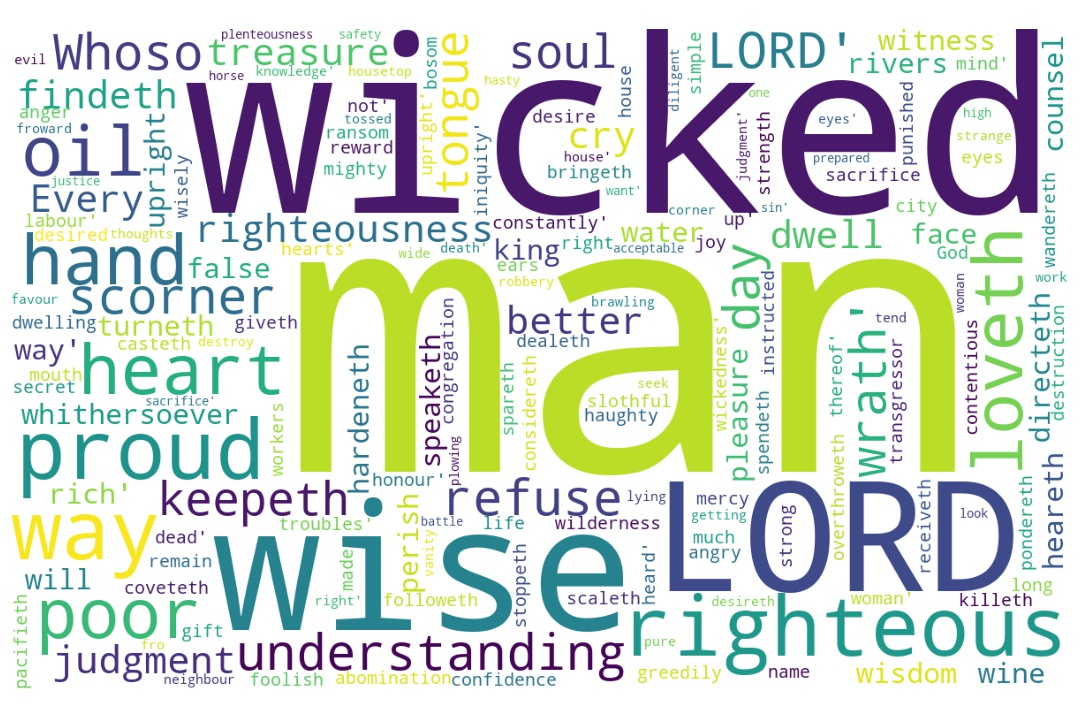
\includegraphics[width=\linewidth]{20OT-Proverbs/Proverb21-WordCloud.jpg}
  \caption{Proverb 21 Word Cloud}
  \label{fig:Proverb 21 word Cloud}
\end{figure}

\marginpar{\scriptsize \centering \fcolorbox{bone}{lime}{\textbf{GOD IN CONTROL OF ALL}}\\ (Proverb 21:1-31) \begin{compactenum}[I.][8]
    \item The \textbf{King's Heart} \index[scripture]{Proverbs!Pro 21:01} (Pro 21:1)
    \item The \textbf{Lord's Hand} \index[scripture]{Proverbs!Pro 21:04} (Pro 21:4)
    \item The \textbf{Look that is High} \index[scripture]{Proverbs!Pro 21:04} (Pro 21:4)
    \item \textbf{Lust that is Hasty} \index[scripture]{Proverbs!Pro 21:05} (Pro 21:5)
    \item \textbf{Languish on the Housetop} \index[scripture]{Proverbs!Pro 21:05} (Pro 21:9)
    \item The \textbf{Lament Unheard} \index[scripture]{Proverbs!Pro 21:13} (Pro 21:13)
    \item The \textbf{Life that is Honored} \index[scripture]{Proverbs!Pro 21:21} (Pro 21:21)
\end{compactenum}}


\marginpar{\scriptsize \centering \fcolorbox{bone}{yellow}{\textbf{LIST OF 13}}\\ (Proverb 21:1-31) \begin{compactenum}[I.][13]
    \item A \textbf{Man} \index[scripture]{Proverbs!Pro 21:02} (Proverbs 21:2)
    \item A \textbf{Proud Heart} \index[scripture]{Proverbs!Pro 21:04} (Proverbs 21:4)
    \item A \textbf{Lying Tongue} \index[scripture]{Proverbs!Pro 21:06} (Proverbs 21:6)
    \item A \textbf{Vanity} \index[scripture]{Proverbs!Pro 21:06} (Proverbs 21:6)
    \item A \textbf{Corner of a House} \index[scripture]{Proverbs!Pro 21:09} (Proverbs 21:9)
    \item A \textbf{Brawling Woman} \index[scripture]{Proverbs!Pro 21:09} (Proverbs 21:9)
    \item A \textbf{Wide House} \index[scripture]{Proverbs!Pro 21:09} (Proverbs 21:9)
    \item A \textbf{Gift} \index[scripture]{Proverbs!Pro 21:14} (Proverbs 21:14)
    \item A \textbf{Poor man} \index[scripture]{Proverbs!Pro 21:17} (Proverbs 21:17)
    \item A \textbf{Ransom} \index[scripture]{Proverbs!Pro 21:18} (Proverbs 21:18)
    \item A \textbf{Contentious and angry woman} \index[scripture]{Proverbs!Pro 21:19} (Proverbs 21:19)
    \item A \textbf{Foolish Man} \index[scripture]{Proverbs!Pro 21:20} (Proverbs 21:20)
    \item A \textbf{Wicked Mind} \index[scripture]{Proverbs!Pro 21:27} (Proverbs 21:27)
\end{compactenum} }

\footnote{\textcolor[cmyk]{0.99998,1,0,0}{\hyperlink{TOC}{Return to end of Table of Contents.}}}\footnote{\href{https://audiobible.com/bible/proverbs_21.html}{\textcolor[cmyk]{0.99998,1,0,0}{Proverbs Audio}}}\textcolor[cmyk]{0.99998,1,0,0}{The \fcolorbox{bone}{lime}{king's heart} \emph{is} in the hand of the LORD, \emph{as} the rivers of water: he turneth it \fcolorbox{bone}{MYGOLD}{whithersoever} he will.}\footnote{\textbf{2 Samuel 14:1} - Now Joab the son of Zeruiah perceived that the king’s heart was toward Absalom.}\footnote{\textbf{Ezra 7:27} - Blessed be the LORD God of our fathers, which hath put such a thing as this in the king’s heart, to beautify the house of the LORD which is in Jerusalem:}
[2] \textcolor[cmyk]{0.99998,1,0,0}{Every way of \fcolorbox{bone}{bone}{a}  man \emph{is} right in his own eyes: but the LORD pondereth the hearts.}\footnote{\textbf{Deuteronomy 12:8} - Ye shall not do after all the things that we do here this day, every man whatsoever is right in his own eyes.}\footnote{\textbf{Judges 17:6} - In those days there was no king in Israel, but every man did that which was right in his own eyes.}\footnote{\textbf{Judges 21:25} - In those days there was no king in Israel: every man did that which was right in his own eyes.}\footnote{\textbf{Proverb 12:15} - The way of a fool is right in his own eyes: but he that hearkeneth unto counsel is wise.}
[3] \textcolor[cmyk]{0.99998,1,0,0}{To do justice and judgment \emph{is} more acceptable to the LORD than sacrifice.}
[4] \textcolor[cmyk]{0.99998,1,0,0}{An \fcolorbox{bone}{lime}{high look}, and \fcolorbox{bone}{bone}{a}  proud heart, \emph{and} the plowing of the wicked, \emph{is} sin.}
[5] \textcolor[cmyk]{0.99998,1,0,0}{The thoughts of the diligent \emph{tend} only to \fcolorbox{bone}{MYGOLD}{plenteousness}; but of every one \emph{that} \emph{is} \fcolorbox{bone}{lime}{hasty only to want}.}
[6] \textcolor[cmyk]{0.99998,1,0,0}{The getting of treasures by \fcolorbox{bone}{bone}{a}  lying tongue \emph{is} \fcolorbox{bone}{bone}{a}  vanity tossed to and fro of them that seek death.}
[7] \textcolor[cmyk]{0.99998,1,0,0}{The robbery of the wicked shall destroy them; because they refuse to do judgment.}
[8] \textcolor[cmyk]{0.99998,1,0,0}{The way of man \emph{is} froward and strange: but \emph{as} \emph{for} the pure, his work \emph{is} right.}
[9] \textcolor[cmyk]{0.99998,1,0,0}{\emph{It} \emph{is} better to dwell in \fcolorbox{bone}{bone}{a}  \fcolorbox{bone}{lime}{corner of the housetop}, than with \fcolorbox{bone}{bone}{a}  brawling woman in \fcolorbox{bone}{bone}{a} wide house.}
[10] \textcolor[cmyk]{0.99998,1,0,0}{The soul of the wicked desireth evil: his neighbour findeth no favour in his eyes.}
[11] \textcolor[cmyk]{0.99998,1,0,0}{When the scorner is punished, the simple is made wise: and when the wise is instructed, he receiveth knowledge.}
[12] \textcolor[cmyk]{0.99998,1,0,0}{The righteous \emph{man} wisely considereth the house of the wicked: \emph{but} \emph{God} overthroweth the wicked for \emph{their} wickedness.}
[13] \textcolor[cmyk]{0.99998,1,0,0}{Whoso stoppeth his ears at \fcolorbox{bone}{lime}{the cry of the poor}, he also shall cry himself, but shall not be heard.}
[14] \textcolor[cmyk]{0.99998,1,0,0}{A gift in secret pacifieth anger: and \fcolorbox{bone}{bone}{a} reward in the bosom strong wrath.}
[15] \textcolor[cmyk]{0.99998,1,0,0}{\emph{It} \emph{is} joy to the just to do judgment: but destruction \emph{shall} \emph{be} to the workers of iniquity.}
[16] \textcolor[cmyk]{0.99998,1,0,0}{The man that wandereth out of the way of \fcolorbox{bone}{MYGOLD}{understanding} shall remain in the congregation of the dead.}
[17] \textcolor[cmyk]{0.99998,1,0,0}{He that loveth pleasure \emph{shall} \emph{be} \fcolorbox{bone}{bone}{a} poor man: he that loveth wine and oil shall not be rich.}
[18] \textcolor[cmyk]{0.99998,1,0,0}{The wicked \emph{shall} \emph{be} \fcolorbox{bone}{bone}{a} ransom for the righteous, and the transgressor for the upright.}
[19] \textcolor[cmyk]{0.99998,1,0,0}{\emph{It} \emph{is} better to dwell in the wilderness, than with \fcolorbox{bone}{bone}{a} contentious and an angry woman.}
[20] \textcolor[cmyk]{0.99998,1,0,0}{\emph{There} \emph{is} treasure to be desired and oil in the dwelling of the wise; but \fcolorbox{bone}{bone}{a} foolish man spendeth it up.}
[21] \textcolor[cmyk]{0.99998,1,0,0}{He that followeth after \fcolorbox{bone}{MYGOLD}{righteousness} and mercy findeth life, \fcolorbox{bone}{MYGOLD}{righteousness}, and \fcolorbox{bone}{lime}{honour}.}
[22] \textcolor[cmyk]{0.99998,1,0,0}{A wise \emph{man} scaleth the city of the mighty, and casteth down the strength of the confidence thereof.}
[23] \textcolor[cmyk]{0.99998,1,0,0}{Whoso keepeth his mouth and his tongue keepeth his soul from troubles.}
[24] \textcolor[cmyk]{0.99998,1,0,0}{Proud \emph{and} haughty scorner \emph{is} his name, who dealeth in proud wrath.}
[25] \textcolor[cmyk]{0.99998,1,0,0}{The desire of the slothful killeth him; for his hands refuse to labour.}
[26] \textcolor[cmyk]{0.99998,1,0,0}{He coveteth greedily all the day long: but the righteous giveth and spareth not.}
[27] \textcolor[cmyk]{0.99998,1,0,0}{The sacrifice of the wicked \emph{is} abomination: how much more, \emph{when} he bringeth it with \fcolorbox{bone}{bone}{a} wicked mind?}
[28] \textcolor[cmyk]{0.99998,1,0,0}{A false witness shall perish: but the man that heareth speaketh constantly.}
[29] \textcolor[cmyk]{0.99998,1,0,0}{A wicked man hardeneth his face: but \emph{as} \emph{for} the upright, he directeth his way.}
[30] \textcolor[cmyk]{0.99998,1,0,0}{\emph{There} \emph{is} no wisdom nor \fcolorbox{bone}{MYGOLD}{understanding} nor counsel against the LORD.}
[31] \textcolor[cmyk]{0.99998,1,0,0}{The horse \emph{is} prepared against the day of battle: but safety \emph{is} of the LORD.}




\index[NWIV]{21!Proverbs!Pro 21:1}\index[AWIP]{The!Proverbs!Pro 21:1}\index[AWIP]{king's!Proverbs!Pro 21:1}\index[AWIP]{heart!Proverbs!Pro 21:1}\index[AWIP]{\emph{is}!Proverbs!Pro 21:1}\index[AWIP]{in!Proverbs!Pro 21:1}\index[AWIP]{the!Proverbs!Pro 21:1}\index[AWIP]{the!Proverbs!Pro 21:1 (2)}\index[AWIP]{the!Proverbs!Pro 21:1 (3)}\index[AWIP]{hand!Proverbs!Pro 21:1}\index[AWIP]{of!Proverbs!Pro 21:1}\index[AWIP]{of!Proverbs!Pro 21:1 (2)}\index[AWIP]{LORD!Proverbs!Pro 21:1}\index[AWIP]{\emph{as}!Proverbs!Pro 21:1}\index[AWIP]{rivers!Proverbs!Pro 21:1}\index[AWIP]{water!Proverbs!Pro 21:1}\index[AWIP]{he!Proverbs!Pro 21:1}\index[AWIP]{he!Proverbs!Pro 21:1 (2)}\index[AWIP]{turneth!Proverbs!Pro 21:1}\index[AWIP]{it!Proverbs!Pro 21:1}\index[AWIP]{whithersoever!Proverbs!Pro 21:1}\index[AWIP]{will!Proverbs!Pro 21:1}\index[AWIP]{\emph{is}!Proverbs!Pro 21:1}\index[AWIP]{\emph{as}!Proverbs!Pro 21:1}

\index[NWIV]{17!Proverbs!Pro 21:2}\index[AWIP]{Every!Proverbs!Pro 21:2}\index[AWIP]{way!Proverbs!Pro 21:2}\index[AWIP]{of!Proverbs!Pro 21:2}\index[AWIP]{a!Proverbs!Pro 21:2}\index[AWIP]{man!Proverbs!Pro 21:2}\index[AWIP]{\emph{is}!Proverbs!Pro 21:2}\index[AWIP]{right!Proverbs!Pro 21:2}\index[AWIP]{in!Proverbs!Pro 21:2}\index[AWIP]{his!Proverbs!Pro 21:2}\index[AWIP]{own!Proverbs!Pro 21:2}\index[AWIP]{eyes!Proverbs!Pro 21:2}\index[AWIP]{but!Proverbs!Pro 21:2}\index[AWIP]{the!Proverbs!Pro 21:2}\index[AWIP]{the!Proverbs!Pro 21:2 (2)}\index[AWIP]{LORD!Proverbs!Pro 21:2}\index[AWIP]{pondereth!Proverbs!Pro 21:2}\index[AWIP]{hearts!Proverbs!Pro 21:2}\index[AWIP]{\emph{is}!Proverbs!Pro 21:2}

\index[NWIV]{13!Proverbs!Pro 21:3}\index[AWIP]{To!Proverbs!Pro 21:3}\index[AWIP]{do!Proverbs!Pro 21:3}\index[AWIP]{justice!Proverbs!Pro 21:3}\index[AWIP]{and!Proverbs!Pro 21:3}\index[AWIP]{judgment!Proverbs!Pro 21:3}\index[AWIP]{\emph{is}!Proverbs!Pro 21:3}\index[AWIP]{more!Proverbs!Pro 21:3}\index[AWIP]{acceptable!Proverbs!Pro 21:3}\index[AWIP]{to!Proverbs!Pro 21:3}\index[AWIP]{the!Proverbs!Pro 21:3}\index[AWIP]{LORD!Proverbs!Pro 21:3}\index[AWIP]{than!Proverbs!Pro 21:3}\index[AWIP]{sacrifice!Proverbs!Pro 21:3}\index[AWIP]{\emph{is}!Proverbs!Pro 21:3}

\index[NWIV]{15!Proverbs!Pro 21:4}\index[AWIP]{An!Proverbs!Pro 21:4}\index[AWIP]{high!Proverbs!Pro 21:4}\index[AWIP]{look!Proverbs!Pro 21:4}\index[AWIP]{and!Proverbs!Pro 21:4}\index[AWIP]{a!Proverbs!Pro 21:4}\index[AWIP]{proud!Proverbs!Pro 21:4}\index[AWIP]{heart!Proverbs!Pro 21:4}\index[AWIP]{\emph{and}!Proverbs!Pro 21:4}\index[AWIP]{the!Proverbs!Pro 21:4}\index[AWIP]{the!Proverbs!Pro 21:4 (2)}\index[AWIP]{plowing!Proverbs!Pro 21:4}\index[AWIP]{of!Proverbs!Pro 21:4}\index[AWIP]{wicked!Proverbs!Pro 21:4}\index[AWIP]{\emph{is}!Proverbs!Pro 21:4}\index[AWIP]{sin!Proverbs!Pro 21:4}\index[AWIP]{\emph{and}!Proverbs!Pro 21:4}\index[AWIP]{\emph{is}!Proverbs!Pro 21:4}

\index[NWIV]{19!Proverbs!Pro 21:5}\index[AWIP]{The!Proverbs!Pro 21:5}\index[AWIP]{thoughts!Proverbs!Pro 21:5}\index[AWIP]{of!Proverbs!Pro 21:5}\index[AWIP]{of!Proverbs!Pro 21:5 (2)}\index[AWIP]{the!Proverbs!Pro 21:5}\index[AWIP]{diligent!Proverbs!Pro 21:5}\index[AWIP]{\emph{tend}!Proverbs!Pro 21:5}\index[AWIP]{only!Proverbs!Pro 21:5}\index[AWIP]{only!Proverbs!Pro 21:5 (2)}\index[AWIP]{to!Proverbs!Pro 21:5}\index[AWIP]{to!Proverbs!Pro 21:5 (2)}\index[AWIP]{plenteousness!Proverbs!Pro 21:5}\index[AWIP]{but!Proverbs!Pro 21:5}\index[AWIP]{every!Proverbs!Pro 21:5}\index[AWIP]{one!Proverbs!Pro 21:5}\index[AWIP]{\emph{that}!Proverbs!Pro 21:5}\index[AWIP]{\emph{is}!Proverbs!Pro 21:5}\index[AWIP]{hasty!Proverbs!Pro 21:5}\index[AWIP]{want!Proverbs!Pro 21:5}\index[AWIP]{\emph{tend}!Proverbs!Pro 21:5}\index[AWIP]{\emph{that}!Proverbs!Pro 21:5}\index[AWIP]{\emph{is}!Proverbs!Pro 21:5}

\index[NWIV]{20!Proverbs!Pro 21:6}\index[AWIP]{The!Proverbs!Pro 21:6}\index[AWIP]{getting!Proverbs!Pro 21:6}\index[AWIP]{of!Proverbs!Pro 21:6}\index[AWIP]{of!Proverbs!Pro 21:6 (2)}\index[AWIP]{treasures!Proverbs!Pro 21:6}\index[AWIP]{by!Proverbs!Pro 21:6}\index[AWIP]{a!Proverbs!Pro 21:6}\index[AWIP]{a!Proverbs!Pro 21:6 (2)}\index[AWIP]{lying!Proverbs!Pro 21:6}\index[AWIP]{tongue!Proverbs!Pro 21:6}\index[AWIP]{\emph{is}!Proverbs!Pro 21:6}\index[AWIP]{vanity!Proverbs!Pro 21:6}\index[AWIP]{tossed!Proverbs!Pro 21:6}\index[AWIP]{to!Proverbs!Pro 21:6}\index[AWIP]{and!Proverbs!Pro 21:6}\index[AWIP]{fro!Proverbs!Pro 21:6}\index[AWIP]{them!Proverbs!Pro 21:6}\index[AWIP]{that!Proverbs!Pro 21:6}\index[AWIP]{seek!Proverbs!Pro 21:6}\index[AWIP]{death!Proverbs!Pro 21:6}\index[AWIP]{\emph{is}!Proverbs!Pro 21:6}

\index[NWIV]{14!Proverbs!Pro 21:7}\index[AWIP]{The!Proverbs!Pro 21:7}\index[AWIP]{robbery!Proverbs!Pro 21:7}\index[AWIP]{of!Proverbs!Pro 21:7}\index[AWIP]{the!Proverbs!Pro 21:7}\index[AWIP]{wicked!Proverbs!Pro 21:7}\index[AWIP]{shall!Proverbs!Pro 21:7}\index[AWIP]{destroy!Proverbs!Pro 21:7}\index[AWIP]{them!Proverbs!Pro 21:7}\index[AWIP]{because!Proverbs!Pro 21:7}\index[AWIP]{they!Proverbs!Pro 21:7}\index[AWIP]{refuse!Proverbs!Pro 21:7}\index[AWIP]{to!Proverbs!Pro 21:7}\index[AWIP]{do!Proverbs!Pro 21:7}\index[AWIP]{judgment!Proverbs!Pro 21:7}

\index[NWIV]{17!Proverbs!Pro 21:8}\index[AWIP]{The!Proverbs!Pro 21:8}\index[AWIP]{way!Proverbs!Pro 21:8}\index[AWIP]{of!Proverbs!Pro 21:8}\index[AWIP]{man!Proverbs!Pro 21:8}\index[AWIP]{\emph{is}!Proverbs!Pro 21:8}\index[AWIP]{\emph{is}!Proverbs!Pro 21:8 (2)}\index[AWIP]{froward!Proverbs!Pro 21:8}\index[AWIP]{and!Proverbs!Pro 21:8}\index[AWIP]{strange!Proverbs!Pro 21:8}\index[AWIP]{but!Proverbs!Pro 21:8}\index[AWIP]{\emph{as}!Proverbs!Pro 21:8}\index[AWIP]{\emph{for}!Proverbs!Pro 21:8}\index[AWIP]{the!Proverbs!Pro 21:8}\index[AWIP]{pure!Proverbs!Pro 21:8}\index[AWIP]{his!Proverbs!Pro 21:8}\index[AWIP]{work!Proverbs!Pro 21:8}\index[AWIP]{right!Proverbs!Pro 21:8}\index[AWIP]{\emph{is}!Proverbs!Pro 21:8}\index[AWIP]{\emph{is}!Proverbs!Pro 21:8 (2)}\index[AWIP]{\emph{as}!Proverbs!Pro 21:8}\index[AWIP]{\emph{for}!Proverbs!Pro 21:8}

\index[NWIV]{20!Proverbs!Pro 21:9}\index[AWIP]{\emph{It}!Proverbs!Pro 21:9}\index[AWIP]{\emph{is}!Proverbs!Pro 21:9}\index[AWIP]{better!Proverbs!Pro 21:9}\index[AWIP]{to!Proverbs!Pro 21:9}\index[AWIP]{dwell!Proverbs!Pro 21:9}\index[AWIP]{in!Proverbs!Pro 21:9}\index[AWIP]{in!Proverbs!Pro 21:9 (2)}\index[AWIP]{a!Proverbs!Pro 21:9}\index[AWIP]{a!Proverbs!Pro 21:9 (2)}\index[AWIP]{a!Proverbs!Pro 21:9 (3)}\index[AWIP]{corner!Proverbs!Pro 21:9}\index[AWIP]{of!Proverbs!Pro 21:9}\index[AWIP]{the!Proverbs!Pro 21:9}\index[AWIP]{housetop!Proverbs!Pro 21:9}\index[AWIP]{than!Proverbs!Pro 21:9}\index[AWIP]{with!Proverbs!Pro 21:9}\index[AWIP]{brawling!Proverbs!Pro 21:9}\index[AWIP]{woman!Proverbs!Pro 21:9}\index[AWIP]{wide!Proverbs!Pro 21:9}\index[AWIP]{house!Proverbs!Pro 21:9}\index[AWIP]{\emph{It}!Proverbs!Pro 21:9}\index[AWIP]{\emph{is}!Proverbs!Pro 21:9}

\index[NWIV]{15!Proverbs!Pro 21:10}\index[AWIP]{The!Proverbs!Pro 21:10}\index[AWIP]{soul!Proverbs!Pro 21:10}\index[AWIP]{of!Proverbs!Pro 21:10}\index[AWIP]{the!Proverbs!Pro 21:10}\index[AWIP]{wicked!Proverbs!Pro 21:10}\index[AWIP]{desireth!Proverbs!Pro 21:10}\index[AWIP]{evil!Proverbs!Pro 21:10}\index[AWIP]{his!Proverbs!Pro 21:10}\index[AWIP]{his!Proverbs!Pro 21:10 (2)}\index[AWIP]{neighbour!Proverbs!Pro 21:10}\index[AWIP]{findeth!Proverbs!Pro 21:10}\index[AWIP]{no!Proverbs!Pro 21:10}\index[AWIP]{favour!Proverbs!Pro 21:10}\index[AWIP]{in!Proverbs!Pro 21:10}\index[AWIP]{eyes!Proverbs!Pro 21:10}

\index[NWIV]{19!Proverbs!Pro 21:11}\index[AWIP]{When!Proverbs!Pro 21:11}\index[AWIP]{the!Proverbs!Pro 21:11}\index[AWIP]{the!Proverbs!Pro 21:11 (2)}\index[AWIP]{the!Proverbs!Pro 21:11 (3)}\index[AWIP]{scorner!Proverbs!Pro 21:11}\index[AWIP]{is!Proverbs!Pro 21:11}\index[AWIP]{is!Proverbs!Pro 21:11 (2)}\index[AWIP]{is!Proverbs!Pro 21:11 (3)}\index[AWIP]{punished!Proverbs!Pro 21:11}\index[AWIP]{simple!Proverbs!Pro 21:11}\index[AWIP]{made!Proverbs!Pro 21:11}\index[AWIP]{wise!Proverbs!Pro 21:11}\index[AWIP]{wise!Proverbs!Pro 21:11 (2)}\index[AWIP]{and!Proverbs!Pro 21:11}\index[AWIP]{when!Proverbs!Pro 21:11}\index[AWIP]{instructed!Proverbs!Pro 21:11}\index[AWIP]{he!Proverbs!Pro 21:11}\index[AWIP]{receiveth!Proverbs!Pro 21:11}\index[AWIP]{knowledge!Proverbs!Pro 21:11}

\index[NWIV]{18!Proverbs!Pro 21:12}\index[AWIP]{The!Proverbs!Pro 21:12}\index[AWIP]{righteous!Proverbs!Pro 21:12}\index[AWIP]{\emph{man}!Proverbs!Pro 21:12}\index[AWIP]{wisely!Proverbs!Pro 21:12}\index[AWIP]{considereth!Proverbs!Pro 21:12}\index[AWIP]{the!Proverbs!Pro 21:12}\index[AWIP]{the!Proverbs!Pro 21:12 (2)}\index[AWIP]{the!Proverbs!Pro 21:12 (3)}\index[AWIP]{house!Proverbs!Pro 21:12}\index[AWIP]{of!Proverbs!Pro 21:12}\index[AWIP]{wicked!Proverbs!Pro 21:12}\index[AWIP]{wicked!Proverbs!Pro 21:12 (2)}\index[AWIP]{\emph{but}!Proverbs!Pro 21:12}\index[AWIP]{\emph{God}!Proverbs!Pro 21:12}\index[AWIP]{overthroweth!Proverbs!Pro 21:12}\index[AWIP]{for!Proverbs!Pro 21:12}\index[AWIP]{\emph{their}!Proverbs!Pro 21:12}\index[AWIP]{wickedness!Proverbs!Pro 21:12}\index[AWIP]{\emph{man}!Proverbs!Pro 21:12}\index[AWIP]{\emph{but}!Proverbs!Pro 21:12}\index[AWIP]{\emph{God}!Proverbs!Pro 21:12}\index[AWIP]{\emph{their}!Proverbs!Pro 21:12}

\index[NWIV]{20!Proverbs!Pro 21:13}\index[AWIP]{Whoso!Proverbs!Pro 21:13}\index[AWIP]{stoppeth!Proverbs!Pro 21:13}\index[AWIP]{his!Proverbs!Pro 21:13}\index[AWIP]{ears!Proverbs!Pro 21:13}\index[AWIP]{at!Proverbs!Pro 21:13}\index[AWIP]{the!Proverbs!Pro 21:13}\index[AWIP]{the!Proverbs!Pro 21:13 (2)}\index[AWIP]{cry!Proverbs!Pro 21:13}\index[AWIP]{cry!Proverbs!Pro 21:13 (2)}\index[AWIP]{of!Proverbs!Pro 21:13}\index[AWIP]{poor!Proverbs!Pro 21:13}\index[AWIP]{he!Proverbs!Pro 21:13}\index[AWIP]{also!Proverbs!Pro 21:13}\index[AWIP]{shall!Proverbs!Pro 21:13}\index[AWIP]{shall!Proverbs!Pro 21:13 (2)}\index[AWIP]{himself!Proverbs!Pro 21:13}\index[AWIP]{but!Proverbs!Pro 21:13}\index[AWIP]{not!Proverbs!Pro 21:13}\index[AWIP]{be!Proverbs!Pro 21:13}\index[AWIP]{heard!Proverbs!Pro 21:13}

\index[NWIV]{14!Proverbs!Pro 21:14}\index[AWIP]{A!Proverbs!Pro 21:14}\index[AWIP]{gift!Proverbs!Pro 21:14}\index[AWIP]{in!Proverbs!Pro 21:14}\index[AWIP]{in!Proverbs!Pro 21:14 (2)}\index[AWIP]{secret!Proverbs!Pro 21:14}\index[AWIP]{pacifieth!Proverbs!Pro 21:14}\index[AWIP]{anger!Proverbs!Pro 21:14}\index[AWIP]{and!Proverbs!Pro 21:14}\index[AWIP]{a!Proverbs!Pro 21:14}\index[AWIP]{reward!Proverbs!Pro 21:14}\index[AWIP]{the!Proverbs!Pro 21:14}\index[AWIP]{bosom!Proverbs!Pro 21:14}\index[AWIP]{strong!Proverbs!Pro 21:14}\index[AWIP]{wrath!Proverbs!Pro 21:14}

\index[NWIV]{18!Proverbs!Pro 21:15}\index[AWIP]{\emph{It}!Proverbs!Pro 21:15}\index[AWIP]{\emph{is}!Proverbs!Pro 21:15}\index[AWIP]{joy!Proverbs!Pro 21:15}\index[AWIP]{to!Proverbs!Pro 21:15}\index[AWIP]{to!Proverbs!Pro 21:15 (2)}\index[AWIP]{to!Proverbs!Pro 21:15 (3)}\index[AWIP]{the!Proverbs!Pro 21:15}\index[AWIP]{the!Proverbs!Pro 21:15 (2)}\index[AWIP]{just!Proverbs!Pro 21:15}\index[AWIP]{do!Proverbs!Pro 21:15}\index[AWIP]{judgment!Proverbs!Pro 21:15}\index[AWIP]{but!Proverbs!Pro 21:15}\index[AWIP]{destruction!Proverbs!Pro 21:15}\index[AWIP]{\emph{shall}!Proverbs!Pro 21:15}\index[AWIP]{\emph{be}!Proverbs!Pro 21:15}\index[AWIP]{workers!Proverbs!Pro 21:15}\index[AWIP]{of!Proverbs!Pro 21:15}\index[AWIP]{iniquity!Proverbs!Pro 21:15}\index[AWIP]{\emph{It}!Proverbs!Pro 21:15}\index[AWIP]{\emph{is}!Proverbs!Pro 21:15}\index[AWIP]{\emph{shall}!Proverbs!Pro 21:15}\index[AWIP]{\emph{be}!Proverbs!Pro 21:15}

\index[NWIV]{18!Proverbs!Pro 21:16}\index[AWIP]{The!Proverbs!Pro 21:16}\index[AWIP]{man!Proverbs!Pro 21:16}\index[AWIP]{that!Proverbs!Pro 21:16}\index[AWIP]{wandereth!Proverbs!Pro 21:16}\index[AWIP]{out!Proverbs!Pro 21:16}\index[AWIP]{of!Proverbs!Pro 21:16}\index[AWIP]{of!Proverbs!Pro 21:16 (2)}\index[AWIP]{of!Proverbs!Pro 21:16 (3)}\index[AWIP]{the!Proverbs!Pro 21:16}\index[AWIP]{the!Proverbs!Pro 21:16 (2)}\index[AWIP]{the!Proverbs!Pro 21:16 (3)}\index[AWIP]{way!Proverbs!Pro 21:16}\index[AWIP]{understanding!Proverbs!Pro 21:16}\index[AWIP]{shall!Proverbs!Pro 21:16}\index[AWIP]{remain!Proverbs!Pro 21:16}\index[AWIP]{in!Proverbs!Pro 21:16}\index[AWIP]{congregation!Proverbs!Pro 21:16}\index[AWIP]{dead!Proverbs!Pro 21:16}

\index[NWIV]{19!Proverbs!Pro 21:17}\index[AWIP]{He!Proverbs!Pro 21:17}\index[AWIP]{that!Proverbs!Pro 21:17}\index[AWIP]{that!Proverbs!Pro 21:17 (2)}\index[AWIP]{loveth!Proverbs!Pro 21:17}\index[AWIP]{loveth!Proverbs!Pro 21:17 (2)}\index[AWIP]{pleasure!Proverbs!Pro 21:17}\index[AWIP]{\emph{shall}!Proverbs!Pro 21:17}\index[AWIP]{\emph{be}!Proverbs!Pro 21:17}\index[AWIP]{a!Proverbs!Pro 21:17}\index[AWIP]{poor!Proverbs!Pro 21:17}\index[AWIP]{man!Proverbs!Pro 21:17}\index[AWIP]{he!Proverbs!Pro 21:17}\index[AWIP]{wine!Proverbs!Pro 21:17}\index[AWIP]{and!Proverbs!Pro 21:17}\index[AWIP]{oil!Proverbs!Pro 21:17}\index[AWIP]{shall!Proverbs!Pro 21:17}\index[AWIP]{not!Proverbs!Pro 21:17}\index[AWIP]{be!Proverbs!Pro 21:17}\index[AWIP]{rich!Proverbs!Pro 21:17}\index[AWIP]{\emph{shall}!Proverbs!Pro 21:17}\index[AWIP]{\emph{be}!Proverbs!Pro 21:17}

\index[NWIV]{15!Proverbs!Pro 21:18}\index[AWIP]{The!Proverbs!Pro 21:18}\index[AWIP]{wicked!Proverbs!Pro 21:18}\index[AWIP]{\emph{shall}!Proverbs!Pro 21:18}\index[AWIP]{\emph{be}!Proverbs!Pro 21:18}\index[AWIP]{a!Proverbs!Pro 21:18}\index[AWIP]{ransom!Proverbs!Pro 21:18}\index[AWIP]{for!Proverbs!Pro 21:18}\index[AWIP]{for!Proverbs!Pro 21:18 (2)}\index[AWIP]{the!Proverbs!Pro 21:18}\index[AWIP]{the!Proverbs!Pro 21:18 (2)}\index[AWIP]{the!Proverbs!Pro 21:18 (3)}\index[AWIP]{righteous!Proverbs!Pro 21:18}\index[AWIP]{and!Proverbs!Pro 21:18}\index[AWIP]{transgressor!Proverbs!Pro 21:18}\index[AWIP]{upright!Proverbs!Pro 21:18}\index[AWIP]{\emph{shall}!Proverbs!Pro 21:18}\index[AWIP]{\emph{be}!Proverbs!Pro 21:18}

\index[NWIV]{16!Proverbs!Pro 21:19}\index[AWIP]{\emph{It}!Proverbs!Pro 21:19}\index[AWIP]{\emph{is}!Proverbs!Pro 21:19}\index[AWIP]{better!Proverbs!Pro 21:19}\index[AWIP]{to!Proverbs!Pro 21:19}\index[AWIP]{dwell!Proverbs!Pro 21:19}\index[AWIP]{in!Proverbs!Pro 21:19}\index[AWIP]{the!Proverbs!Pro 21:19}\index[AWIP]{wilderness!Proverbs!Pro 21:19}\index[AWIP]{than!Proverbs!Pro 21:19}\index[AWIP]{with!Proverbs!Pro 21:19}\index[AWIP]{a!Proverbs!Pro 21:19}\index[AWIP]{contentious!Proverbs!Pro 21:19}\index[AWIP]{and!Proverbs!Pro 21:19}\index[AWIP]{an!Proverbs!Pro 21:19}\index[AWIP]{angry!Proverbs!Pro 21:19}\index[AWIP]{woman!Proverbs!Pro 21:19}\index[AWIP]{\emph{It}!Proverbs!Pro 21:19}\index[AWIP]{\emph{is}!Proverbs!Pro 21:19}

\index[NWIV]{21!Proverbs!Pro 21:20}\index[AWIP]{\emph{There}!Proverbs!Pro 21:20}\index[AWIP]{\emph{is}!Proverbs!Pro 21:20}\index[AWIP]{treasure!Proverbs!Pro 21:20}\index[AWIP]{to!Proverbs!Pro 21:20}\index[AWIP]{be!Proverbs!Pro 21:20}\index[AWIP]{desired!Proverbs!Pro 21:20}\index[AWIP]{and!Proverbs!Pro 21:20}\index[AWIP]{oil!Proverbs!Pro 21:20}\index[AWIP]{in!Proverbs!Pro 21:20}\index[AWIP]{the!Proverbs!Pro 21:20}\index[AWIP]{the!Proverbs!Pro 21:20 (2)}\index[AWIP]{dwelling!Proverbs!Pro 21:20}\index[AWIP]{of!Proverbs!Pro 21:20}\index[AWIP]{wise!Proverbs!Pro 21:20}\index[AWIP]{but!Proverbs!Pro 21:20}\index[AWIP]{a!Proverbs!Pro 21:20}\index[AWIP]{foolish!Proverbs!Pro 21:20}\index[AWIP]{man!Proverbs!Pro 21:20}\index[AWIP]{spendeth!Proverbs!Pro 21:20}\index[AWIP]{it!Proverbs!Pro 21:20}\index[AWIP]{up!Proverbs!Pro 21:20}\index[AWIP]{\emph{There}!Proverbs!Pro 21:20}\index[AWIP]{\emph{is}!Proverbs!Pro 21:20}

\index[NWIV]{12!Proverbs!Pro 21:21}\index[AWIP]{He!Proverbs!Pro 21:21}\index[AWIP]{that!Proverbs!Pro 21:21}\index[AWIP]{followeth!Proverbs!Pro 21:21}\index[AWIP]{after!Proverbs!Pro 21:21}\index[AWIP]{righteousness!Proverbs!Pro 21:21}\index[AWIP]{righteousness!Proverbs!Pro 21:21 (2)}\index[AWIP]{and!Proverbs!Pro 21:21}\index[AWIP]{and!Proverbs!Pro 21:21 (2)}\index[AWIP]{mercy!Proverbs!Pro 21:21}\index[AWIP]{findeth!Proverbs!Pro 21:21}\index[AWIP]{life!Proverbs!Pro 21:21}\index[AWIP]{honour!Proverbs!Pro 21:21}

\index[NWIV]{18!Proverbs!Pro 21:22}\index[AWIP]{A!Proverbs!Pro 21:22}\index[AWIP]{wise!Proverbs!Pro 21:22}\index[AWIP]{\emph{man}!Proverbs!Pro 21:22}\index[AWIP]{scaleth!Proverbs!Pro 21:22}\index[AWIP]{the!Proverbs!Pro 21:22}\index[AWIP]{the!Proverbs!Pro 21:22 (2)}\index[AWIP]{the!Proverbs!Pro 21:22 (3)}\index[AWIP]{the!Proverbs!Pro 21:22 (4)}\index[AWIP]{city!Proverbs!Pro 21:22}\index[AWIP]{of!Proverbs!Pro 21:22}\index[AWIP]{of!Proverbs!Pro 21:22 (2)}\index[AWIP]{mighty!Proverbs!Pro 21:22}\index[AWIP]{and!Proverbs!Pro 21:22}\index[AWIP]{casteth!Proverbs!Pro 21:22}\index[AWIP]{down!Proverbs!Pro 21:22}\index[AWIP]{strength!Proverbs!Pro 21:22}\index[AWIP]{confidence!Proverbs!Pro 21:22}\index[AWIP]{thereof!Proverbs!Pro 21:22}\index[AWIP]{\emph{man}!Proverbs!Pro 21:22}

\index[NWIV]{12!Proverbs!Pro 21:23}\index[AWIP]{Whoso!Proverbs!Pro 21:23}\index[AWIP]{keepeth!Proverbs!Pro 21:23}\index[AWIP]{keepeth!Proverbs!Pro 21:23 (2)}\index[AWIP]{his!Proverbs!Pro 21:23}\index[AWIP]{his!Proverbs!Pro 21:23 (2)}\index[AWIP]{his!Proverbs!Pro 21:23 (3)}\index[AWIP]{mouth!Proverbs!Pro 21:23}\index[AWIP]{and!Proverbs!Pro 21:23}\index[AWIP]{tongue!Proverbs!Pro 21:23}\index[AWIP]{soul!Proverbs!Pro 21:23}\index[AWIP]{from!Proverbs!Pro 21:23}\index[AWIP]{troubles!Proverbs!Pro 21:23}

\index[NWIV]{12!Proverbs!Pro 21:24}\index[AWIP]{Proud!Proverbs!Pro 21:24}\index[AWIP]{\emph{and}!Proverbs!Pro 21:24}\index[AWIP]{haughty!Proverbs!Pro 21:24}\index[AWIP]{scorner!Proverbs!Pro 21:24}\index[AWIP]{\emph{is}!Proverbs!Pro 21:24}\index[AWIP]{his!Proverbs!Pro 21:24}\index[AWIP]{name!Proverbs!Pro 21:24}\index[AWIP]{who!Proverbs!Pro 21:24}\index[AWIP]{dealeth!Proverbs!Pro 21:24}\index[AWIP]{in!Proverbs!Pro 21:24}\index[AWIP]{proud!Proverbs!Pro 21:24}\index[AWIP]{wrath!Proverbs!Pro 21:24}\index[AWIP]{\emph{and}!Proverbs!Pro 21:24}\index[AWIP]{\emph{is}!Proverbs!Pro 21:24}

\index[NWIV]{13!Proverbs!Pro 21:25}\index[AWIP]{The!Proverbs!Pro 21:25}\index[AWIP]{desire!Proverbs!Pro 21:25}\index[AWIP]{of!Proverbs!Pro 21:25}\index[AWIP]{the!Proverbs!Pro 21:25}\index[AWIP]{slothful!Proverbs!Pro 21:25}\index[AWIP]{killeth!Proverbs!Pro 21:25}\index[AWIP]{him!Proverbs!Pro 21:25}\index[AWIP]{for!Proverbs!Pro 21:25}\index[AWIP]{his!Proverbs!Pro 21:25}\index[AWIP]{hands!Proverbs!Pro 21:25}\index[AWIP]{refuse!Proverbs!Pro 21:25}\index[AWIP]{to!Proverbs!Pro 21:25}\index[AWIP]{labour!Proverbs!Pro 21:25}

\index[NWIV]{14!Proverbs!Pro 21:26}\index[AWIP]{He!Proverbs!Pro 21:26}\index[AWIP]{coveteth!Proverbs!Pro 21:26}\index[AWIP]{greedily!Proverbs!Pro 21:26}\index[AWIP]{all!Proverbs!Pro 21:26}\index[AWIP]{the!Proverbs!Pro 21:26}\index[AWIP]{the!Proverbs!Pro 21:26 (2)}\index[AWIP]{day!Proverbs!Pro 21:26}\index[AWIP]{long!Proverbs!Pro 21:26}\index[AWIP]{but!Proverbs!Pro 21:26}\index[AWIP]{righteous!Proverbs!Pro 21:26}\index[AWIP]{giveth!Proverbs!Pro 21:26}\index[AWIP]{and!Proverbs!Pro 21:26}\index[AWIP]{spareth!Proverbs!Pro 21:26}\index[AWIP]{not!Proverbs!Pro 21:26}

\index[NWIV]{18!Proverbs!Pro 21:27}\index[AWIP]{The!Proverbs!Pro 21:27}\index[AWIP]{sacrifice!Proverbs!Pro 21:27}\index[AWIP]{of!Proverbs!Pro 21:27}\index[AWIP]{the!Proverbs!Pro 21:27}\index[AWIP]{wicked!Proverbs!Pro 21:27}\index[AWIP]{wicked!Proverbs!Pro 21:27 (2)}\index[AWIP]{\emph{is}!Proverbs!Pro 21:27}\index[AWIP]{abomination!Proverbs!Pro 21:27}\index[AWIP]{how!Proverbs!Pro 21:27}\index[AWIP]{much!Proverbs!Pro 21:27}\index[AWIP]{more!Proverbs!Pro 21:27}\index[AWIP]{\emph{when}!Proverbs!Pro 21:27}\index[AWIP]{he!Proverbs!Pro 21:27}\index[AWIP]{bringeth!Proverbs!Pro 21:27}\index[AWIP]{it!Proverbs!Pro 21:27}\index[AWIP]{with!Proverbs!Pro 21:27}\index[AWIP]{a!Proverbs!Pro 21:27}\index[AWIP]{mind?!Proverbs!Pro 21:27}\index[AWIP]{\emph{is}!Proverbs!Pro 21:27}\index[AWIP]{\emph{when}!Proverbs!Pro 21:27}

\index[NWIV]{12!Proverbs!Pro 21:28}\index[AWIP]{A!Proverbs!Pro 21:28}\index[AWIP]{false!Proverbs!Pro 21:28}\index[AWIP]{witness!Proverbs!Pro 21:28}\index[AWIP]{shall!Proverbs!Pro 21:28}\index[AWIP]{perish!Proverbs!Pro 21:28}\index[AWIP]{but!Proverbs!Pro 21:28}\index[AWIP]{the!Proverbs!Pro 21:28}\index[AWIP]{man!Proverbs!Pro 21:28}\index[AWIP]{that!Proverbs!Pro 21:28}\index[AWIP]{heareth!Proverbs!Pro 21:28}\index[AWIP]{speaketh!Proverbs!Pro 21:28}\index[AWIP]{constantly!Proverbs!Pro 21:28}

\index[NWIV]{15!Proverbs!Pro 21:29}\index[AWIP]{A!Proverbs!Pro 21:29}\index[AWIP]{wicked!Proverbs!Pro 21:29}\index[AWIP]{man!Proverbs!Pro 21:29}\index[AWIP]{hardeneth!Proverbs!Pro 21:29}\index[AWIP]{his!Proverbs!Pro 21:29}\index[AWIP]{his!Proverbs!Pro 21:29 (2)}\index[AWIP]{face!Proverbs!Pro 21:29}\index[AWIP]{but!Proverbs!Pro 21:29}\index[AWIP]{\emph{as}!Proverbs!Pro 21:29}\index[AWIP]{\emph{for}!Proverbs!Pro 21:29}\index[AWIP]{the!Proverbs!Pro 21:29}\index[AWIP]{upright!Proverbs!Pro 21:29}\index[AWIP]{he!Proverbs!Pro 21:29}\index[AWIP]{directeth!Proverbs!Pro 21:29}\index[AWIP]{way!Proverbs!Pro 21:29}\index[AWIP]{\emph{as}!Proverbs!Pro 21:29}\index[AWIP]{\emph{for}!Proverbs!Pro 21:29}

\index[NWIV]{11!Proverbs!Pro 21:30}\index[AWIP]{\emph{There}!Proverbs!Pro 21:30}\index[AWIP]{\emph{is}!Proverbs!Pro 21:30}\index[AWIP]{no!Proverbs!Pro 21:30}\index[AWIP]{wisdom!Proverbs!Pro 21:30}\index[AWIP]{nor!Proverbs!Pro 21:30}\index[AWIP]{nor!Proverbs!Pro 21:30 (2)}\index[AWIP]{understanding!Proverbs!Pro 21:30}\index[AWIP]{counsel!Proverbs!Pro 21:30}\index[AWIP]{against!Proverbs!Pro 21:30}\index[AWIP]{the!Proverbs!Pro 21:30}\index[AWIP]{LORD!Proverbs!Pro 21:30}\index[AWIP]{\emph{There}!Proverbs!Pro 21:30}\index[AWIP]{\emph{is}!Proverbs!Pro 21:30}

\index[NWIV]{15!Proverbs!Pro 21:31}\index[AWIP]{The!Proverbs!Pro 21:31}\index[AWIP]{horse!Proverbs!Pro 21:31}\index[AWIP]{\emph{is}!Proverbs!Pro 21:31}\index[AWIP]{\emph{is}!Proverbs!Pro 21:31 (2)}\index[AWIP]{prepared!Proverbs!Pro 21:31}\index[AWIP]{against!Proverbs!Pro 21:31}\index[AWIP]{the!Proverbs!Pro 21:31}\index[AWIP]{the!Proverbs!Pro 21:31 (2)}\index[AWIP]{day!Proverbs!Pro 21:31}\index[AWIP]{of!Proverbs!Pro 21:31}\index[AWIP]{of!Proverbs!Pro 21:31 (2)}\index[AWIP]{battle!Proverbs!Pro 21:31}\index[AWIP]{but!Proverbs!Pro 21:31}\index[AWIP]{safety!Proverbs!Pro 21:31}\index[AWIP]{LORD!Proverbs!Pro 21:31}\index[AWIP]{\emph{is}!Proverbs!Pro 21:31}\index[AWIP]{\emph{is}!Proverbs!Pro 21:31 (2)}


%%%%%%%%%%%%%%%%%%%%%%%%%%%%%%%%%%%%%%%

\index[DOCTRINES]{Practicology!Doctrine of Safety!!Proverbs!Pro 21:31}

\index[DOCTRINES]{Practicology!Doctrine of Scorners!!Proverbs!Pro 21:11}
\index[DOCTRINES]{Practicology!Doctrine of Scorners!!Proverbs!Pro 21:24}

\index[DOCTRINES]{Practicology!Doctrine of Secrecy!!Proverbs!Pro 21:24}


\index[DOCTRINES]{Practicology!Doctrine of Simplicity!!Proverbs!Pro 21:11}

\section{Proverbs 21 Outlines}

\subsection{My Outlines}

\subsubsection{God in Control of All}
\index[speaker]{Keith Anthony!Proverb 21 (God in Control of All)}
\index[series]{Proverbs (Keith Anthony)!Pro 21 (God in Control of All)}
\index[date]{2016/05/21!Proverb 21 (God in Control of All) (Keith Anthony)}
\textbf{Introduction:} Despite the events that seemingly appear to be out of control and in the hands of the ungodly, God is in control and working all things out according to his plans. As Christians following Gods will, further, we have the promise that it will all to our good.
\index[scripture]{Romans!Rom 08:28} (Romans 8:28)
\begin{compactenum}[I.]
    \item The \textbf{King's Heart} \index[scripture]{Proverbs!Pro 21:01} (Pro 21:1)
    \item The \textbf{Lord's Hand} \index[scripture]{Proverbs!Pro 21:04} (Pro 21:4)
    \item The \textbf{Look that is High} \index[scripture]{Proverbs!Pro 21:04} (Pro 21:4)
    \item \textbf{Lust that is Hasty} \index[scripture]{Proverbs!Pro 21:05} (Pro 21:5)
    \item \textbf{Languish on the Housetop} \index[scripture]{Proverbs!Pro 21:05} (Pro 21:9)
    \item The \textbf{Lament Unheard} \index[scripture]{Proverbs!Pro 21:13} (Pro 21:13)
    \item The \textbf{Life that is Honored} \index[scripture]{Proverbs!Pro 21:21} (Pro 21:21)
\end{compactenum}

\subsubsection{A List of 13}
\index[speaker]{Keith Anthony!Proverb 21 (A List of 13)}
\index[series]{Proverbs (Keith Anthony)!Pro 21 (A List of 13)}
\index[date]{2018/05/21!Proverb 21 (A List of 13) (Keith Anthony)}
\textbf{Introduction : }The word ``a'' (lower-case and not italics) is found 13 times in the chapter.
\begin{compactenum}[I.][13]
    \item A \textbf{Man} \index[scripture]{Proverbs!Pro 21:02} (Pro 21:2)
    \item A \textbf{Proud Heart} \index[scripture]{Proverbs!Pro 21:04} (Pro 21:4)
    \item A \textbf{Lying Tongue} \index[scripture]{Proverbs!Pro 21:06} (Pro 21:6)
    \item A \textbf{Vanity} \index[scripture]{Proverbs!Pro 21:06} (Pro 21:6)
    \item A \textbf{Corner of a House} \index[scripture]{Proverbs!Pro 21:09} (Pro 21:9)
    \item A \textbf{Brawling Woman} \index[scripture]{Proverbs!Pro 21:09} (Pro 21:9)
    \item A \textbf{Wide House} \index[scripture]{Proverbs!Pro 21:09} (Pro 21:9)
    \item A \textbf{Gift} \index[scripture]{Proverbs!Pro 21:14} (Pro 21:14)
    \item A \textbf{Poor man} \index[scripture]{Proverbs!Pro 21:17} (Pro 21:17)
    \item A \textbf{Ransom} \index[scripture]{Proverbs!Pro 21:18} (Pro 21:18)
    \item A \textbf{Contentious and angry woman} \index[scripture]{Proverbs!Pro 21:19} (Pro 21:19)
    \item A \textbf{Foolish Man} \index[scripture]{Proverbs!Pro 21:20} (Pro 21:20)
    \item A \textbf{Wicked Mind} \index[scripture]{Proverbs!Pro 21:27} (Pro 21:27)
\end{compactenum}

\subsection{Outlines from Others}


\section{Proverb 21 Comments}

\subsection{Numeric Nuggets}
\textbf{13: } Verses 3 and 25 have 13 words. Verses 3, 14, 25, and 26 have13 unique words. The word ``a'' is found 13 times in the chapter. The 13-letter words ``whithersoever,'' ``plenteousness,'' ``understanding,'' and ``righteousness'' are used in the chapter.


\subsection{Proverb 21 Repeated Phrases}


%%%%%%%%%%
%%%%%%%%%%
\normalsize
 
\begin{center}
\begin{longtable}{|p{3.0in}|p{0.5in}|}
\caption[Proverb 21 Repeated Phrases]{Proverb 21 Repeated Phrases}\label{table:Repeated Phrases Proverb 21} \\
\hline \multicolumn{1}{|c|}{\textbf{Phrase}} & \multicolumn{1}{c|}{\textbf{Frequency}} \\ \hline 
\endfirsthead
 
\multicolumn{2}{c}
{{\bfseries \tablename\ \thetable{} -- continued from previous page}} \\  
\hline \multicolumn{1}{|c|}{\textbf{Phrase}} & \multicolumn{1}{c|}{\textbf{Frequency}} \\ \hline 
\endhead
 
\hline \multicolumn{2}{c}{{ }} \\ \hline
\endfoot 
of the & 16\\ \hline 
the wicked & 6\\ \hline 
in the & 5\\ \hline 
the LORD & 5\\ \hline 
of the wicked & 5\\ \hline 
way of & 3\\ \hline 
but the & 3\\ \hline 
to the & 3\\ \hline 
\emph{It} \emph{is} & 3\\ \hline 
with a & 3\\ \hline 
\emph{shall} \emph{be} & 3\\ \hline 
\end{longtable}
\end{center}



%%%%%%%%%%
%%%%%%%%%%



%\newpage
\section{Proverb 21 Statistics}

%%%%%%%%%%%%%%%%%%%%%%%%%%%
%%%%% Word Statistics
%%%%%%%%%%%%%%%%%%%%%%%%%%

\normalsize
\subsection{Chapter Word Statistics}


%%%%%%%%%%
%%%%%%%%%%
 
\begin{center}
\begin{longtable}{l|c|c|c|c}
\caption[Stats for Proverb 21]{Stats for Proverb 21} \label{table:Stats for Proverb 21} \\ 
\hline \multicolumn{1}{|c|}{\textbf{Verse(s)}} & \multicolumn{1}{|c|}{\textbf{Count}} & \multicolumn{1}{|c|}{\textbf{Unique}} & \multicolumn{1}{|c|}{\textbf{Italics}} & \multicolumn{1}{|c|}{\textbf{Uniq Italic}}  \\ \hline 
\endfirsthead
 
\multicolumn{5}{c}
{{\bfseries \tablename\ \thetable{} -- continued from previous page}} \\  
\hline \multicolumn{1}{|c|}{\textbf{Verse(s)}} & \multicolumn{1}{|c|}{\textbf{Count}} & \multicolumn{1}{|c|}{\textbf{Unique}} & \multicolumn{1}{|c|}{\textbf{Italics}} & \multicolumn{1}{|c|}{\textbf{Uniq Italic}}  \\ \hline 
\endhead
 
\hline \multicolumn{5}{|r|}{{Continued if needed}} \\ \hline
\endfoot 
1 & 21 & 17 & 2 & 2\\ \hline
2 & 17 & 16 & 1 & 1\\ \hline
3 & 13 & 13 & 1 & 1\\ \hline
4 & 15 & 14 & 2 & 2\\ \hline
5 & 19 & 16 & 3 & 3\\ \hline
6 & 20 & 18 & 1 & 1\\ \hline
7 & 14 & 14 & 0 & 0\\ \hline
8 & 17 & 16 & 4 & 3\\ \hline
9 & 20 & 17 & 2 & 2\\ \hline
10 & 15 & 14 & 0 & 0\\ \hline
11 & 19 & 14 & 0 & 0\\ \hline
12 & 18 & 15 & 4 & 4\\ \hline
13 & 20 & 17 & 0 & 0\\ \hline
14 & 14 & 13 & 0 & 0\\ \hline
15 & 18 & 15 & 4 & 4\\ \hline
16 & 18 & 14 & 0 & 0\\ \hline
17 & 19 & 17 & 2 & 2\\ \hline
18 & 15 & 12 & 2 & 2\\ \hline
19 & 16 & 16 & 2 & 2\\ \hline
20 & 21 & 20 & 2 & 2\\ \hline
21 & 12 & 10 & 0 & 0\\ \hline
22 & 18 & 14 & 1 & 1\\ \hline
23 & 12 & 9 & 0 & 0\\ \hline
24 & 12 & 12 & 2 & 2\\ \hline
25 & 13 & 13 & 0 & 0\\ \hline
26 & 14 & 13 & 0 & 0\\ \hline
27 & 18 & 17 & 2 & 2\\ \hline
28 & 12 & 12 & 0 & 0\\ \hline
29 & 15 & 14 & 2 & 2\\ \hline
30 & 11 & 10 & 2 & 2\\ \hline
31 & 15 & 12 & 2 & 1\\ \hline
\hline \hline
Total & 501 & 229 & 43 & 15




\end{longtable}
\end{center}

%%%%%%%%%%
%%%%%%%%%%


\subsection{Words by Frequency}

\begin{center}
\begin{longtable}{l|r}
\caption[Word Frequencies in Proverb 21]{Word Frequencies in Proverb 21} \label{table:WordsIn-Proverb-21} \\ 
\hline \multicolumn{1}{|c|}{\textbf{Word}} & \multicolumn{1}{c|}{\textbf{Frequency}} \\ \hline 
\endfirsthead
  
\multicolumn{2}{c}  
{{\bfseries \tablename\ \thetable{} -- continued from previous page}} \\   
\hline \multicolumn{1}{|c|}{\textbf{Word}} & \multicolumn{1}{c|}{\textbf{Frequency}} \\ \hline   
\endhead  
  
\hline \multicolumn{2}{|r|}{{Continue}} \\ \hline  
\endfoot  
  
\hline \hline  
\endlastfoot  
  
the & 46\\ \hline 
of & 25\\ \hline 
\emph{is} & 17\\ \hline 
and & 15\\ \hline 
a & 13\\ \hline 
The & 12\\ \hline 
his & 12\\ \hline 
to & 12\\ \hline 
in & 11\\ \hline 
but & 10\\ \hline 
wicked & 9\\ \hline 
he & 7\\ \hline 
man & 7\\ \hline 
that & 6\\ \hline 
shall & 6\\ \hline 
LORD & 5\\ \hline 
way & 4\\ \hline 
wise & 4\\ \hline 
for & 4\\ \hline 
A & 4\\ \hline 
\emph{as} & 3\\ \hline 
it & 3\\ \hline 
do & 3\\ \hline 
judgment & 3\\ \hline 
than & 3\\ \hline 
\emph{It} & 3\\ \hline 
with & 3\\ \hline 
is & 3\\ \hline 
righteous & 3\\ \hline 
not & 3\\ \hline 
be & 3\\ \hline 
\emph{shall} & 3\\ \hline 
\emph{be} & 3\\ \hline 
He & 3\\ \hline 
heart & 2\\ \hline 
right & 2\\ \hline 
eyes & 2\\ \hline 
more & 2\\ \hline 
sacrifice & 2\\ \hline 
proud & 2\\ \hline 
\emph{and} & 2\\ \hline 
only & 2\\ \hline 
tongue & 2\\ \hline 
them & 2\\ \hline 
refuse & 2\\ \hline 
\emph{for} & 2\\ \hline 
better & 2\\ \hline 
dwell & 2\\ \hline 
woman & 2\\ \hline 
house & 2\\ \hline 
soul & 2\\ \hline 
findeth & 2\\ \hline 
no & 2\\ \hline 
scorner & 2\\ \hline 
\emph{man} & 2\\ \hline 
Whoso & 2\\ \hline 
cry & 2\\ \hline 
poor & 2\\ \hline 
wrath & 2\\ \hline 
understanding & 2\\ \hline 
loveth & 2\\ \hline 
oil & 2\\ \hline 
upright & 2\\ \hline 
\emph{There} & 2\\ \hline 
righteousness & 2\\ \hline 
keepeth & 2\\ \hline 
day & 2\\ \hline 
nor & 2\\ \hline 
against & 2\\ \hline 
king's & 1\\ \hline 
hand & 1\\ \hline 
rivers & 1\\ \hline 
water & 1\\ \hline 
turneth & 1\\ \hline 
whithersoever & 1\\ \hline 
will & 1\\ \hline 
Every & 1\\ \hline 
own & 1\\ \hline 
pondereth & 1\\ \hline 
hearts & 1\\ \hline 
To & 1\\ \hline 
justice & 1\\ \hline 
acceptable & 1\\ \hline 
An & 1\\ \hline 
high & 1\\ \hline 
look & 1\\ \hline 
plowing & 1\\ \hline 
sin & 1\\ \hline 
thoughts & 1\\ \hline 
diligent & 1\\ \hline 
\emph{tend} & 1\\ \hline 
plenteousness & 1\\ \hline 
every & 1\\ \hline 
one & 1\\ \hline 
\emph{that} & 1\\ \hline 
hasty & 1\\ \hline 
want & 1\\ \hline 
getting & 1\\ \hline 
treasures & 1\\ \hline 
by & 1\\ \hline 
lying & 1\\ \hline 
vanity & 1\\ \hline 
tossed & 1\\ \hline 
fro & 1\\ \hline 
seek & 1\\ \hline 
death & 1\\ \hline 
robbery & 1\\ \hline 
destroy & 1\\ \hline 
because & 1\\ \hline 
they & 1\\ \hline 
froward & 1\\ \hline 
strange & 1\\ \hline 
pure & 1\\ \hline 
work & 1\\ \hline 
corner & 1\\ \hline 
housetop & 1\\ \hline 
brawling & 1\\ \hline 
wide & 1\\ \hline 
desireth & 1\\ \hline 
evil & 1\\ \hline 
neighbour & 1\\ \hline 
favour & 1\\ \hline 
When & 1\\ \hline 
punished & 1\\ \hline 
simple & 1\\ \hline 
made & 1\\ \hline 
when & 1\\ \hline 
instructed & 1\\ \hline 
receiveth & 1\\ \hline 
knowledge & 1\\ \hline 
wisely & 1\\ \hline 
considereth & 1\\ \hline 
\emph{but} & 1\\ \hline 
\emph{God} & 1\\ \hline 
overthroweth & 1\\ \hline 
\emph{their} & 1\\ \hline 
wickedness & 1\\ \hline 
stoppeth & 1\\ \hline 
ears & 1\\ \hline 
at & 1\\ \hline 
also & 1\\ \hline 
himself & 1\\ \hline 
heard & 1\\ \hline 
gift & 1\\ \hline 
secret & 1\\ \hline 
pacifieth & 1\\ \hline 
anger & 1\\ \hline 
reward & 1\\ \hline 
bosom & 1\\ \hline 
strong & 1\\ \hline 
joy & 1\\ \hline 
just & 1\\ \hline 
destruction & 1\\ \hline 
workers & 1\\ \hline 
iniquity & 1\\ \hline 
wandereth & 1\\ \hline 
out & 1\\ \hline 
remain & 1\\ \hline 
congregation & 1\\ \hline 
dead & 1\\ \hline 
pleasure & 1\\ \hline 
wine & 1\\ \hline 
rich & 1\\ \hline 
ransom & 1\\ \hline 
transgressor & 1\\ \hline 
wilderness & 1\\ \hline 
contentious & 1\\ \hline 
an & 1\\ \hline 
angry & 1\\ \hline 
treasure & 1\\ \hline 
desired & 1\\ \hline 
dwelling & 1\\ \hline 
foolish & 1\\ \hline 
spendeth & 1\\ \hline 
up & 1\\ \hline 
followeth & 1\\ \hline 
after & 1\\ \hline 
mercy & 1\\ \hline 
life & 1\\ \hline 
honour & 1\\ \hline 
scaleth & 1\\ \hline 
city & 1\\ \hline 
mighty & 1\\ \hline 
casteth & 1\\ \hline 
down & 1\\ \hline 
strength & 1\\ \hline 
confidence & 1\\ \hline 
thereof & 1\\ \hline 
mouth & 1\\ \hline 
from & 1\\ \hline 
troubles & 1\\ \hline 
Proud & 1\\ \hline 
haughty & 1\\ \hline 
name & 1\\ \hline 
who & 1\\ \hline 
dealeth & 1\\ \hline 
desire & 1\\ \hline 
slothful & 1\\ \hline 
killeth & 1\\ \hline 
him & 1\\ \hline 
hands & 1\\ \hline 
labour & 1\\ \hline 
coveteth & 1\\ \hline 
greedily & 1\\ \hline 
all & 1\\ \hline 
long & 1\\ \hline 
giveth & 1\\ \hline 
spareth & 1\\ \hline 
abomination & 1\\ \hline 
how & 1\\ \hline 
much & 1\\ \hline 
\emph{when} & 1\\ \hline 
bringeth & 1\\ \hline 
mind & 1\\ \hline 
false & 1\\ \hline 
witness & 1\\ \hline 
perish & 1\\ \hline 
heareth & 1\\ \hline 
speaketh & 1\\ \hline 
constantly & 1\\ \hline 
hardeneth & 1\\ \hline 
face & 1\\ \hline 
directeth & 1\\ \hline 
wisdom & 1\\ \hline 
counsel & 1\\ \hline 
horse & 1\\ \hline 
prepared & 1\\ \hline 
battle & 1\\ \hline 
safety & 1\\ \hline 
\end{longtable}  
\end{center}  


  
\normalsize  

  
  


\subsection{Words Alphabetically}

\begin{center}
\begin{longtable}{l|r}
\caption[Word Frequencies in Proverb 21]{Word Frequencies in Proverb 21} \label{table:WordsIn-Proverb-21} \\ 
\hline \multicolumn{1}{|c|}{\textbf{Word}} & \multicolumn{1}{c|}{\textbf{Frequency}} \\ \hline 
\endfirsthead
  
\multicolumn{2}{c}  
{{\bfseries \tablename\ \thetable{} -- continued from previous page}} \\   
\hline \multicolumn{1}{|c|}{\textbf{Word}} & \multicolumn{1}{c|}{\textbf{Frequency}} \\ \hline   
\endhead  
  
\hline \multicolumn{2}{|r|}{{Continue}} \\ \hline  
\endfoot  
  
\hline \hline  
\endlastfoot  
  
A & 4\\ \hline 
An & 1\\ \hline 
Every & 1\\ \hline 
He & 3\\ \hline 
LORD & 5\\ \hline 
Proud & 1\\ \hline 
The & 12\\ \hline 
To & 1\\ \hline 
When & 1\\ \hline 
Whoso & 2\\ \hline 
\emph{God} & 1\\ \hline 
\emph{It} & 3\\ \hline 
\emph{There} & 2\\ \hline 
\emph{and} & 2\\ \hline 
\emph{as} & 3\\ \hline 
\emph{be} & 3\\ \hline 
\emph{but} & 1\\ \hline 
\emph{for} & 2\\ \hline 
\emph{is} & 17\\ \hline 
\emph{man} & 2\\ \hline 
\emph{shall} & 3\\ \hline 
\emph{tend} & 1\\ \hline 
\emph{that} & 1\\ \hline 
\emph{their} & 1\\ \hline 
\emph{when} & 1\\ \hline 
a & 13\\ \hline 
abomination & 1\\ \hline 
acceptable & 1\\ \hline 
after & 1\\ \hline 
against & 2\\ \hline 
all & 1\\ \hline 
also & 1\\ \hline 
an & 1\\ \hline 
and & 15\\ \hline 
anger & 1\\ \hline 
angry & 1\\ \hline 
at & 1\\ \hline 
battle & 1\\ \hline 
be & 3\\ \hline 
because & 1\\ \hline 
better & 2\\ \hline 
bosom & 1\\ \hline 
brawling & 1\\ \hline 
bringeth & 1\\ \hline 
but & 10\\ \hline 
by & 1\\ \hline 
casteth & 1\\ \hline 
city & 1\\ \hline 
confidence & 1\\ \hline 
congregation & 1\\ \hline 
considereth & 1\\ \hline 
constantly & 1\\ \hline 
contentious & 1\\ \hline 
corner & 1\\ \hline 
counsel & 1\\ \hline 
coveteth & 1\\ \hline 
cry & 2\\ \hline 
day & 2\\ \hline 
dead & 1\\ \hline 
dealeth & 1\\ \hline 
death & 1\\ \hline 
desire & 1\\ \hline 
desired & 1\\ \hline 
desireth & 1\\ \hline 
destroy & 1\\ \hline 
destruction & 1\\ \hline 
diligent & 1\\ \hline 
directeth & 1\\ \hline 
do & 3\\ \hline 
down & 1\\ \hline 
dwell & 2\\ \hline 
dwelling & 1\\ \hline 
ears & 1\\ \hline 
every & 1\\ \hline 
evil & 1\\ \hline 
eyes & 2\\ \hline 
face & 1\\ \hline 
false & 1\\ \hline 
favour & 1\\ \hline 
findeth & 2\\ \hline 
followeth & 1\\ \hline 
foolish & 1\\ \hline 
for & 4\\ \hline 
fro & 1\\ \hline 
from & 1\\ \hline 
froward & 1\\ \hline 
getting & 1\\ \hline 
gift & 1\\ \hline 
giveth & 1\\ \hline 
greedily & 1\\ \hline 
hand & 1\\ \hline 
hands & 1\\ \hline 
hardeneth & 1\\ \hline 
hasty & 1\\ \hline 
haughty & 1\\ \hline 
he & 7\\ \hline 
heard & 1\\ \hline 
heareth & 1\\ \hline 
heart & 2\\ \hline 
hearts & 1\\ \hline 
high & 1\\ \hline 
him & 1\\ \hline 
himself & 1\\ \hline 
his & 12\\ \hline 
honour & 1\\ \hline 
horse & 1\\ \hline 
house & 2\\ \hline 
housetop & 1\\ \hline 
how & 1\\ \hline 
in & 11\\ \hline 
iniquity & 1\\ \hline 
instructed & 1\\ \hline 
is & 3\\ \hline 
it & 3\\ \hline 
joy & 1\\ \hline 
judgment & 3\\ \hline 
just & 1\\ \hline 
justice & 1\\ \hline 
keepeth & 2\\ \hline 
killeth & 1\\ \hline 
king's & 1\\ \hline 
knowledge & 1\\ \hline 
labour & 1\\ \hline 
life & 1\\ \hline 
long & 1\\ \hline 
look & 1\\ \hline 
loveth & 2\\ \hline 
lying & 1\\ \hline 
made & 1\\ \hline 
man & 7\\ \hline 
mercy & 1\\ \hline 
mighty & 1\\ \hline 
mind & 1\\ \hline 
more & 2\\ \hline 
mouth & 1\\ \hline 
much & 1\\ \hline 
name & 1\\ \hline 
neighbour & 1\\ \hline 
no & 2\\ \hline 
nor & 2\\ \hline 
not & 3\\ \hline 
of & 25\\ \hline 
oil & 2\\ \hline 
one & 1\\ \hline 
only & 2\\ \hline 
out & 1\\ \hline 
overthroweth & 1\\ \hline 
own & 1\\ \hline 
pacifieth & 1\\ \hline 
perish & 1\\ \hline 
pleasure & 1\\ \hline 
plenteousness & 1\\ \hline 
plowing & 1\\ \hline 
pondereth & 1\\ \hline 
poor & 2\\ \hline 
prepared & 1\\ \hline 
proud & 2\\ \hline 
punished & 1\\ \hline 
pure & 1\\ \hline 
ransom & 1\\ \hline 
receiveth & 1\\ \hline 
refuse & 2\\ \hline 
remain & 1\\ \hline 
reward & 1\\ \hline 
rich & 1\\ \hline 
right & 2\\ \hline 
righteous & 3\\ \hline 
righteousness & 2\\ \hline 
rivers & 1\\ \hline 
robbery & 1\\ \hline 
sacrifice & 2\\ \hline 
safety & 1\\ \hline 
scaleth & 1\\ \hline 
scorner & 2\\ \hline 
secret & 1\\ \hline 
seek & 1\\ \hline 
shall & 6\\ \hline 
simple & 1\\ \hline 
sin & 1\\ \hline 
slothful & 1\\ \hline 
soul & 2\\ \hline 
spareth & 1\\ \hline 
speaketh & 1\\ \hline 
spendeth & 1\\ \hline 
stoppeth & 1\\ \hline 
strange & 1\\ \hline 
strength & 1\\ \hline 
strong & 1\\ \hline 
than & 3\\ \hline 
that & 6\\ \hline 
the & 46\\ \hline 
them & 2\\ \hline 
thereof & 1\\ \hline 
they & 1\\ \hline 
thoughts & 1\\ \hline 
to & 12\\ \hline 
tongue & 2\\ \hline 
tossed & 1\\ \hline 
transgressor & 1\\ \hline 
treasure & 1\\ \hline 
treasures & 1\\ \hline 
troubles & 1\\ \hline 
turneth & 1\\ \hline 
understanding & 2\\ \hline 
up & 1\\ \hline 
upright & 2\\ \hline 
vanity & 1\\ \hline 
wandereth & 1\\ \hline 
want & 1\\ \hline 
water & 1\\ \hline 
way & 4\\ \hline 
when & 1\\ \hline 
whithersoever & 1\\ \hline 
who & 1\\ \hline 
wicked & 9\\ \hline 
wickedness & 1\\ \hline 
wide & 1\\ \hline 
wilderness & 1\\ \hline 
will & 1\\ \hline 
wine & 1\\ \hline 
wisdom & 1\\ \hline 
wise & 4\\ \hline 
wisely & 1\\ \hline 
with & 3\\ \hline 
witness & 1\\ \hline 
woman & 2\\ \hline 
work & 1\\ \hline 
workers & 1\\ \hline 
wrath & 2\\ \hline 
\end{longtable}  
\end{center}  


  
\normalsize  

  
  
\subsection{Word Lengths in Chapter} 
\normalsize 
\begin{center} 
\begin{longtable}{l|p{3.75in}} 
\caption[Words by Length in Proverb 21]{Words by Length in Proverb 21} \label{table:WordsIn-Proverb-21} \\ 
\hline \multicolumn{1}{|c|}{\textbf{Length}} & \multicolumn{1}{c|}{\textbf{Words}} \\ \hline 
\endfirsthead 
 
\multicolumn{2}{c} 
{{\bfseries \tablename\ \thetable{} -- continued from previous page}} \\ 
\hline \multicolumn{1}{|c|}{\textbf{Length}} & \multicolumn{1}{c|}{\textbf{Words}} \\ \hline 
\endhead 
 
\hline \multicolumn{2}{|r|}{{Continued}} \\ \hline 
\endfoot 
 
\hline \hline 
\endlastfoot 
1 & a, A\\ \hline 
2 & \emph{is}, in, of, \emph{as}, he, it, To, do, to, An, by, \emph{It}, no, is, at, be, \emph{be}, He, an, up\\ \hline 
3 & The, the, way, man, his, own, but, and, \emph{and}, sin, one, fro, \emph{for}, \emph{man}, \emph{but}, \emph{God}, for, cry, not, joy, out, oil, who, him, all, day, how, nor\\ \hline 
4 & hand, LORD, will, eyes, more, than, high, look, \emph{tend}, only, \emph{that}, want, them, that, seek, they, pure, work, with, wide, soul, evil, When, made, wise, when, ears, poor, also, gift, just, dead, wine, rich, life, city, down, from, name, long, much, \emph{when}, mind, face\\ \hline 
5 & heart, water, Every, right, proud, every, hasty, lying, death, shall, dwell, woman, house, \emph{their}, Whoso, heard, anger, bosom, wrath, \emph{shall}, angry, \emph{There}, after, mercy, mouth, Proud, hands, false, horse\\ \hline 
6 & king's, rivers, hearts, wicked, tongue, vanity, tossed, refuse, better, corner, favour, simple, wisely, secret, reward, strong, remain, loveth, ransom, honour, mighty, desire, labour, giveth, perish, wisdom, battle, safety\\ \hline 
7 & turneth, justice, plowing, getting, robbery, destroy, because, froward, strange, findeth, scorner, himself, workers, upright, desired, foolish, scaleth, casteth, thereof, keepeth, haughty, dealeth, killeth, spareth, witness, heareth, counsel, against\\ \hline 
8 & judgment, thoughts, diligent, housetop, brawling, desireth, punished, stoppeth, iniquity, pleasure, treasure, dwelling, spendeth, strength, troubles, slothful, coveteth, greedily, bringeth, speaketh, prepared\\ \hline 
9 & pondereth, sacrifice, treasures, neighbour, receiveth, knowledge, righteous, pacifieth, wandereth, followeth, hardeneth, directeth\\ \hline 
10 & acceptable, instructed, wickedness, wilderness, confidence, constantly\\ \hline 
11 & considereth, destruction, contentious, abomination\\ \hline 
12 & overthroweth, congregation, transgressor\\ \hline 
13 & whithersoever, plenteousness, understanding, righteousness\\ \hline 
\end{longtable} 
\end{center} 




%%%%%%%%%%
%%%%%%%%%%
 

%\input{20OT-Proverbs/Example-DEVOTIONAL-Psalm3-DEVOTIONAL-BryanChapel}


%%% For Indexes

%\index[DEVOTIONAL]{TGIF1!Os Hillman (Living for a Cause Greater Than Yourself) - Proverb 19:17!2021/12/21}

%\index[DEVOTIONAL]{TGIF1!Os Hillman (Living for a Cause Greater Than Yourself) - Proverb 19:17!2021/12/21}

















%%% colour: cardinal red - \textcolor[cmyk]{0,0.85,0.70,0.23}{text}


%%%% Example marginpar with a compactenum list --- green color text
%\marginpar{\scriptsize \textcolor[rgb]{0.00,0.545,0.269}{$\rightarrow$7 Abominations: 
%\begin{compactenum}
%	\item A proud look,
%	\item a lying tongue,
%	\item hands that shed innocent blood,
%	\item An heart that deviseth wicked imaginations,
%	\item feet that be swift in running to mischief,
%	\item A false witness that speaketh lies, and
%	\item he that soweth discord among brethren.
%\end{compactenum}}}



%\newpage

%\begin{mdframed}[style=MyFrame]
%\begin{center}
%\begin{longtable}{|p{.5in}|p{3.5in}|}

%\caption[Corruption Alert: Proverbs 18:1]{Corruption Alert: Proverbs 18:1} \label{table:CorruptionProv18:1} \\ 

%\hline  
%\multicolumn{1}{|c|}{\textbf{Version}} & 
%\multicolumn{1}{c|}{\textbf{Corruption}}  \\ \hline 
%\endfirsthead
 
%\multicolumn{2}{c}
%{{\bfseries \tablename\ \thetable{} -- continued from previous page}} \\  \hline  
%\multicolumn{1}{|c|}{\textbf{Version}} & 
%\multicolumn{1}{c|}{\textbf{Corruption}}  \\ \hline 
%\endhead
 
%\hline \multicolumn{2}{|r|}{{Continued on next page}} \\ \hline
%\endfoot 
%\textcolor[rgb]{0.00,0.00,1.00}{AV} & \textcolor[rgb]{0.00,0.00,1.00}{Through desire a man, having separated himself, seeketh \emph{and} intermeddleth with all wisdom.} \\ \hline
%
%ASV &  He that separateth himself seeketh his own desire, And  rageth against all sound wisdom. \\ \hline
%
%CEB &  Unfriendly people look out for themselves; they bicker with sensible people.\\ \hline
%
%ESV & Whoever isolates himself seeks his own desire;  he breaks out against all sound judgment. \\ \hline
%
%NASV &  He who separates himself seeks his own desire, He quarrels against all sound wisdom.\\ \hline
%
%MEV & He who separates himself seeks his own desire; he seeks and quarrels against all wisdom.\\ \hline
%
%NIV &  An unfriendly person pursues selfish ends and against all sound judgment starts quarrels. \\ \hline
%
%NKJV &  A man who isolates himself seeks his own desire; He rages against all wise judgment.\\ \hline
%
%RSV &  He who is estranged seeks pretexts  to break out against all sound judgment.\\ \hline

% \multicolumn{2}{p{4.3in}}{{Modern translations, such as the ASV and others, strike out the first part of the verse, concealing the intent of mankind in genewisdom clearly revealed in scripture. How wonderful is the obfuscated RSV text: ``He who is estranged seeks pretexts.'' What does THAT mean?}} \\ %\hline

%\hline

%\end{longtable}
%\end{center}

%\normalsize 
%\end{mdframed}

%\marginpar{\scriptsize \centering \fcolorbox{black}{lime}{\textbf{OUTIDE THE PLACE OF PROMISE}}\\ (Psalm 137:1--9) 
%\begin{compactenum}[I.][8]
%	\item \textbf{Plight \& Distress} \index[scripture]{Psalms!Psa 137:01} (Psalm 137:1)
%	\item The \textbf{Place Desired} \index[scripture]{Psalms!Psa 137:01} (Psalm 137:1)
%	\item \textbf{Pining \& Despiar} \index[scripture]{Psalms!Psa 137:02} (Psalm 137:2)
%	\item \textbf{Provoked \& Degraded}\index[scripture]{Psalms!Psa 137:03} (Psalm 137:3)
%	\item The \textbf{Predicament Described}\index[scripture]{Psalms!Psa 137:04} (Psalm 137:4)
%	\item A \textbf{Preference Decided}\index[scripture]{Psalms!Psa 137:06} (Psalm 137:6)
%	\item A \textbf{Prediction of Destruction}\index[scripture]{Psalms!Psa 137:08} (Psalm 137:8)
%\end{compactenum} }


%\subsection{Outlines from Others}

%\subsubsection{Words on Wisdom}
%\index[speaker]{John Battles!Proverbs 01 (Words on Wisdom)}
%\index[series]{Proverbs (John Battles)!Proverbs 01 (Words on Wisdom)}
%\index[date]{2016/01/20!Proverbs 01 (Words on Wisdom) (John Battles)}
%\textbf{Lineage}: adpated from S. Conway\\
%\textbf{Introduction}: Proverbs distinctly points out things that a fool does:
%\begin{compactenum}[I.][4]
%	\item \textbf{Welcome to Wisdom} \index[scripture]{Proverbs!Pro 01:01-09}(Proverbs 1:1-9)
%	\item \textbf{Warnings of Wisdom} \index[scripture]{Proverbs!Pro 01:10-19}(Proverbs 1:10-19).
%	\item \textbf{Woe of Wisdom} \index[scripture]{Proverbs!Pro 01:24-32}(Proverbs 1:24-32)
%	\item \textbf{Watchcare of Wisdom} \index[scripture]{Proverbs!Pro 01:33}(Proverbs 1:33).
%\end{compactenum}


%%%%% COLOR FOR MARGINPAR OUTLINES
%% 1  LIME - \marginpar{\scriptsize \centering \fcolorbox{black}{lime}{\textbf{TITLE}}\\ (Passage) 
%% 2. YELLOW - \marginpar{\scriptsize \centering \fcolorbox{black}{yellow}{\textbf{TITLE}}\\ (Passage) 
%% 3. Blue BGND, WHITE LETTERS - \marginpar{\scriptsize \centering \fcolorbox{black}{blue}{\textbf{\textcolor[cmyk]{0,0,0,0}{TITLE}}}\\ (Passage) 
%% 4. black BGND, WHITE LETTERS - \marginpar{\scriptsize \centering \fcolorbox{black}{black}{\textbf{\textcolor[cmyk]{0,0,0,0}{TITLE}}}\\ (Passage) 
%% 5. red BGND, WHITE LETTERS - \marginpar{\scriptsize \centering \fcolorbox{black}{red}{\textbf{\textcolor[cmyk]{0,0,0,0}{TITLE}}}\\ (Passage) 

%%%%%% INCLUSION OF GRAPHIC
%\newpage

%\begin{figure}
%\begin{center}
%\includegraphics[scale=0.5, angle=90]{07OT-Judges/References/b201107i1-large}
%\caption[Summary of the 13 Judges]{Summary of the 13 Judges}
%\label{fig:Summary of the 13 Judges}
%\end{center}
%\end{figure}


%%%%%%%%%%%
%%%%%%%%%%%

% SYTEMATIC THEOLOGY (10 + 2)
% Theology proper – The study of the character of God
% Angelology – The study of angels
% Biblical theology – The study of the Bible
% Christology – The study of Christ
% Ecclesiology – The study of the church
% Eschatology – The study of the end times[5]
% Hamartiology – The study of sin
% Pneumatology – The study of the Holy Spirit
% Soteriology – The study of salvation
% Theological anthropology – The study of the nature of humanity.
% ++
% Moral theology
% Bilical cosomolgy

%%%%%%%%%%%%%%
%%%%%%%%%%%%%%

% \footnote{\href{https://audiobible.com/bible/psalms_91.html}{\textcolor[cmyk]{0.99998,1,0,0}{Psalm 91 Audio}}}

% \marginpar{\scriptsize \centering \fcolorbox{black}{lime}{\textbf{JERUSALEM}}\\
% \fcolorbox{black}{lime}{\textbf{DON'T GO BACK TO EGYPT}} \\ (Isaiah 31:1--9) 

%%%%%%%%%%%%%%
%%% Extra Colors
%%% from https://latexcolor.blogspot.com/2019/10/list-of-latex-colors.html
%%%%%%%%%%%%%%
% \definecolor{champagne}{rgb}{0.97,0.91,0.81}
% \definecolor{bone}{rgb}{0.89,0.85,0.79}
%\titleJE
%

%%%%% EXAMPLE Index entry:
% \index[DOCTRINES]{Eschatology - Millennium!Psalms!Psa 069:036}

%%% for things found 13 times
%\fcolorbox{black}{bone}{TEXT}
\scriptsize

%%%%%%%%%%%%%%%%%%%%%%%%%%%%%
%Indices

\chapter{Indexes}
\printindex[DOCTRINES]
\printindex[scripture]
\printindex[speaker]
%\printindex[series]

\printindex[FACEBOOK]
\printindex[LOCATION]
\printindex[DEVOTIONAL]
\printindex[AWIP]

\printbibliography
\end{document}

